
\chapter{}
	
\heading{ಲೇಡಿ ರಾಮನ್}

ಶ‍್ರೀಮತಿ ಲೋಕಸುಂದರಿ ರಾಮನ್ ಅವರ ಬಗ್ಗೆ ಎರಡು ಮಾತುಗಳು ಇಲ್ಲಿ ಸೂಕ್ತವೆನ್ನಿಸುತ್ತದೆ. ರಾಮನ್ ಅವರ ಬಗ್ಗೆ ಲೋಕ ಸುಂದರಿಯವರಿಗಿದ್ದ ಭಕ್ತಿಯು ಅವರನ್ನು ಹತ್ತಿರದಿಂದ ಬಲ್ಲವರಿಗೆ ಗೋಚರವಾಗುತ್ತಿತ್ತು. ಅನೇಕ ಪ್ರವಾಸಗಳಲ್ಲಿ ತಮ್ಮ ಪತಿಯ ಜೊತೆಗಿದ್ದು ಅವರ ಯೋಗಕ್ಷೇಮವನ್ನು ನೋಡಿಕೊಳ್ಳುತ್ತಿದ್ದರು. ರಾಮನ್ ಅವರ ವೈಜ್ಞಾನಿಕ ಜೀವನಕ್ಕೆ ಯಾವ ಅಡೆತಡೆಗಳೂ ಬಾರದಂತೆ ಕಾಯುವುದೇ ತಮ್ಮ ಜೀವನದ ಸಾರ್ಥಕತೆಯೆಂದು ಅವರು ಬಗೆದಿದ್ದರು. ಪತಿಯಿಂದ ಭಿನ್ನವಾದ ತಮ್ಮ ವ್ಯಕ್ತಿತ್ವವೊಂದಿದೆಯೆಂದು ಸಾರ್ವಜನಿಕವಾಗಿ ಅವರೆಂದಿಗೂ ತೋರಿಸಿಕೊಳ್ಳಲಿಲ್ಲ. ಇದು ಭಾರತೀಯ ಸಂಪ್ರದಾಯಬದ್ಧ ನಾರಿಯ ಗುಣವೆನ್ನಿಸಿದರೂ, ಅವರ ಹತ್ತಿರದವರ ಗಮನವನ್ನು ಗಾಢವಾಗಿ ಸೆಳೆಯುತ್ತಿತ್ತು.

ಲೇಡಿ ರಾಮನ್‍ರವರು ಸೌಮ್ಯ ಸ್ವಭಾವದವರು. ಅವರ ನಡೆನುಡಿಗಳಲ್ಲಿ ಗಾಂಭಿರ್ಯವೂ, ಸಂಸ್ಕೃತಿಯೂ ಕಾಣುತ್ತಿತ್ತು. ಅವರು ಯಾವ ಒಡವೆಯನ್ನೂ ಧರಿಸದೆ ಸಾಧಾರಣ ಸೀರೆಯನ್ನೇ ಉಡುತ್ತಿದ್ದರು. ಅವರಿಗೆ ಅನೇಕ ಭಾಷೆಗಳು ಬರುತ್ತಿದ್ದವು. ತಮಿಳು ಅವರ ಮಾತೃಭಾಷೆ, ಆದರೂ ಬೆಂಗಾಲಿಯನ್ನು ನಿರರ್ಗಳವಾಗಿ ಮಾತನಾಡುತ್ತಿದ್ದರು. ಅವರು ಇಂಗ್ಲಿಷ್, ಕನ್ನಡ, ಹಿಂದಿ ಮತ್ತು ತೆಲುಗು ಭಾಷೆಗಳಲ್ಲಿ ವ್ಯವಹರಿಸಬಲ್ಲವರಾಗಿದ್ದರು. ಮಹಿಳೆಯರು, ಮಕ್ಕಳು ಮತ್ತು ಹಿಂದುಳಿದವರ ಪರವಾಗಿ ಕೆಲಸ ಮಾಡುವ ಅನೇಕ ಸಂಘ ಸಂಸ್ಥೆಗಳ ಚಟುವಟಿಕೆಗಳಲ್ಲಿ ತಮ್ಮನ್ನು ತೊಡಗಿಸಿಕೊಂಡಿದ್ದರು.

\enginline{1936}ರ ಆದಿಯಲ್ಲಿ ಮಹಾತ್ಮಗಾಂಧಿಯವರೊಡನೆ ಲೇಡಿ ರಾಮನ್‍ರವರು ಮಾಡಿದ\break ಸಂಭಾಷಣೆಯಲ್ಲಿ ಅವರ ಅನೇಕ ಆಸಕ್ತಿಗಳೂ, ಸ್ವಭಾವಗಳೂ ಕಾಣುತ್ತವೆ. ಗಾಂಧಿಯವರು, ತಾವು ರಾಮನ್ ಇನ್ಸ್ಟಿಟ್ಯೂಟ್ ಅನ್ನು ನೋಡಲು ಉತ್ಸುಕರಾಗಿರುವುದಾಗಿಯೂ, ಅಲ್ಲಿ ಯಾವುದಾದರೂ ಕಣ್ಸೆಳೆಯುವ ಮ್ಯಾಜಿಕ್ ನೋಡಲಿಚ್ಛಿಸುವುದಾಗಿಯೂ ಹೇಳಿದರು. “ನಿಮ್ಮ ಬಗ್ಗೆ ರಾಮನ್ ಅವರ ಬಾಯಿಂದ ಅನೇಕ ಒಳ್ಳೆಯ ಸಂಗತಿಗಳನ್ನು ಕೇಳಿದ್ದೇನೆ. ಆದರೆ ಅವು ಎಷ್ಟು ಸತ್ಯ ಎಂದು ನನಗೆ ಮನವರಿಕೆಯಾಗಬೇಕಿದೆ. ತಾವು ವಿಜ್ಞಾನದಲ್ಲಿ ಮುಳುಗಿಹೋಗಿದ್ದಾಗ, ನೀವು ಅನೇಕ ಮಾನವತಾವಾದಿ ಚಟುವಟಿಕೆಗಳಲ್ಲಿ ತೊಡಗಿಸಿಕೊಳ್ಳುತ್ತೀರಿ ಎಂದು ರಾಮನ್ ಹೇಳಿದ್ದರು”.

ಲೇಡಿ ರಾಮನ್ \enginline{--} “ನಾನು ನಿಜವಾಗಲೂ ಮಾಡಬಹುದಾದಷ್ಟು ಮಾಡಲಾಗಿಲ್ಲ. ಆದರೆ ಖಾದಿ, ಹರಿಜನೋದ್ಧಾರ ಮತ್ತು ಇಂತಹ ಇತರೆ ಸಾಮಾಜಿಕ ಕಾರ್ಯಗಳಲ್ಲಿ ನನಗೆ ಆಸಕ್ತಿ. ಮಹಾತ್ಮಾಜೀ, ನಿಮಗೇ ತಿಳಿದಿರುವಂತೆ ನಾನು ಅನೇಕ ವರ್ಷಗಳಿಂದ ನೂಲು ತೆಗೆಯುತ್ತಿದ್ದೇನೆ. ಸುಮಾರು ಹದಿನೈದು ವರ್ಷಗಳ ಹಿಂದೆ ನಾನು ನೂಲಿನ ಸಂಗ್ರಹವನ್ನು ಬಟ್ಟೆ ನೇಯ್ದುಕೊಡಲು ನಿಮಗೆ ಕಳುಹಿಸಿದ್ದೆ. ದಿವಂಗತ ಮದನ್ ಲಾಲ ಗಾಂಧಿಯವರು ನೇಯ್ದ ಬಟ್ಟೆಯನ್ನು ನನಗೆ ಕಳುಹಿಸಿದರು. ಆದರೆ ಆಗ ನನ್ನ ಪತಿಯವರಿಗೆ ಚರಕದಲ್ಲಿ ನಂಬಿಕೆ ಇರಲಿಲ್ಲ. ಅವರು ನನ್ನ ಚರಕವನ್ನು ಬಿಸಾಡುತ್ತಿದ್ದರು, ಮುರಿದು ಹಾಕುತ್ತಿದ್ದರು, ಆದರೆ ಇಂದು ಅವರು ಚರಕವನ್ನು ಹೀಯಾಳಿಸುವುದಿಲ್ಲ ಅದರ ಮೇಲೆ ನಂಬಿಕೆ ಬೆಳೆಸಿಕೊಂಡಿರುವುದು ನನಗೆ ಸಂತಸ ತಂದಿದೆ. ನಾನು ಜೀವಿಸಿರುವಾಗಲೇ ಈ ಪರಿವರ್ತನೆಯನ್ನು ನೋಡಿದ್ದೇನೆ”.

ಗಾಂಧಿಯವರು ಹೀಗೆಂದರು “ನನಗೆ ಬಹಳ ಸಂತೋಷವಾಗಿದೆ. ಇರಲಿ ನೀವು ನನಗೆ ಸಣ್ಣದೊಂದು ಕೆಲಸ ಮಾಡಿಕೊಡಿ. ನೀವು ಕಮಲನೆಹರೂ ಅವರನ್ನು ಎಂದಾದರೂ ಭೇಟಿಯಾದ\-ದ್ದುಂಟೇ?” ಲೇಡಿ ರಾಮನ್\enginline{--} “ಮಹಾತ್ಮಾಜೀ ಒಂದೆರಡು ಬಾರಿ ಇರಬಹುದು ಆದರೆ ನನಗೆ ಶ‍್ರೀಮತಿ ನೆಹರೂ ಅವರು ಚೆನ್ನಾಗಿ ಗೊತ್ತು”. ಗಾಂಧಿ \enginline{--} “ಕಮಲ ಅವರು ಎಷ್ಟು ಒಳ್ಳೆಯವರೆಂದು ನಿಮಗೆ ತಿಳಿದಿರಲೇಬೇಕಲ್ಲ. ಅವರು ದೇಶಸೇವೆಗಾಗಿ ತಮ್ಮನ್ನು ತೇಯ್ದುಕೊಂಡರು ಎಂಬುದೂ ತಿಳಿದಿರಬೇಕು. ಆದರೆ ನಾನು ಬಹಳ ಮೌಲ್ಯಕೊಡುವುದು ಅವರ ರಾಜಕೀಯ ಸೇವೆಗಲ್ಲ. ಅವರ ಆಧ್ಯಾತ್ಮ ಸೌಂದರ್ಯಕ್ಕಾಗಿ ಪ್ರತಿಯೊಬ್ಬ ಸ್ತ್ರೀ ಪುರುಷರಿಗೆ ಇದು ಗೊತ್ತಾಗಬೇಕು”.

ಲೇಡಿ ರಾಮನ್ \enginline{--} “ಹೌದು ಅವರ ಸೇವೆಗಳೂ ಮತ್ತು ಅವರ ನೈತಿಕ ಸೌಂದರ್ಯವೂ ನನಗೆ ತಿಳಿದಿದೆ”.

ಗಾಂಧಿ \enginline{--} “ಹಾಗಿದ್ದಾಗ ನೀವು ನನಗೆ ಸಹಾಯಮಾಡಬೇಕು. ಅವರಿಗೊಂದು ಸ್ಮಾರಕವನ್ನು ನಿರ್ಮಿಸಲಿದ್ದೇವೆ.”

ಲೇಡಿ ರಾಮನ್‍ರವರು ಸಂತೋಷದಿಂದ ಒಪ್ಪಿದರು. ಹೀಗೆ ಸಂಭಾಷಣೆಯು ಮುಂದುವರೆಯು\-ತ್ತಿದ್ದಾಗ ರಾಮನ್‍ರವರು ಒಳಗೆ ಬಂದರು. ಸಂಭಾಷಣೆಯು ಹಿಂದಿಯಲ್ಲಿ ನಡೆಯುತ್ತಿತ್ತು. “ಇವಳ ಹಿಂದಿ ಸ್ಫುಟವಾಗಿದೆಯೇ” ಎಂದು ಕೇಳಿದರು.

ಗಾಂಧಿ \enginline{--} “ಬಹಳ ಚೆನ್ನಾಗಿದೆ. ನಿಮ್ಮ ವಿಜ್ಞಾನದಷ್ಟೇ ಚೆನ್ನಾಗಿದೆ”.

ರಾಮನ್ \enginline{--} “ಹೌದು, ಭಾಷೆಗಳನ್ನು ಕಲಿಯುವುದರಲ್ಲಿ ಇವಳಿಗೆ ಬಹಳ ಚುರುಕುತನವಿದೆ. ಇವಳಿಗೆ ಹಿಂದಿಯೂ ಗೊತ್ತು. ಬೆಂಗಾಲಿಯು ಹಿಂದಿಗಿಂತಲೂ ಚೆನ್ನಾಗಿ ಗೊತ್ತು”.

ಗಾಂಧಿ \enginline{--} “ಇರಲೇಬೇಕು. ಹೇಗೂ ಇವರು ಕಲ್ಕತ್ತಾದಲ್ಲಿ ಅನೇಕ ವರ್ಷಗಳು ಇದ್ದರಲ್ಲವೇ”.

ರಾಮನ್ \enginline{--} “ಆ ಕಾರಣಕ್ಕಾಗಿ ಅಲ್ಲ. ನಾನೂ (ಇವಳ ಜೊತೆ) ಇದ್ದೆನಲ್ಲ. ನನಗೆ ಒಂದು ಪದವೂ ಬರುವುದಿಲ್ಲ, ಆದರೆ, ಇವಳು ಇಲ್ಲಿ ಕನ್ನಡವನ್ನು ಕಲಿತು ಬಿಟ್ಟಿದ್ದಾಳೆ. ಕನ್ನಡದಲ್ಲಿ ಮಾತನಾಡಬಲ್ಲಳು”. ಬಳಿಕ ರಾಮನ್‍ರವರು ಭಾರತ ದೇಶಕ್ಕೆ ಯಾವ ಭಾಷೆ ಸೂಕ್ತವೆಂದು ಚರ್ಚಿಸತೊಡಗಿದರು. ಅವರ ಒಲವು ಇಂಗ್ಲಿಷ್‍ನ ಕಡೆಗೆ ಇತ್ತು”. (ಹರಿಜನ್ \enginline{6.6.36})

\newpage

ಲೇಡಿ ರಾಮನ್ ಅವರ ಪ್ರಮುಖ ಆಸಕ್ತಿಯು ರಾಮನ್ ಅವರನ್ನು ನೋಡಿಕೊಳ್ಳುವುದೇ ಆಗಿತ್ತು. ಅವರಿಗೆ ಕಾಲ ಕಾಲಕ್ಕೆ ಊಟೋಪಚಾರಗಳೂ, ಅವರನ್ನು ವಿಶ್ರಾಂತಿ ಪಡೆಯಲು ತಾಕೀತು ಮಾಡುವುದೂ ಇದರಲ್ಲಿ ಸೇರಿತ್ತು. ತಮ್ಮ ಕುಟುಂಬವನ್ನು ಬಹಳ ಅಚ್ಚುಕಟ್ಟಾಗಿ ನಿಭಾಯಿಸಿದರು. ತಮ್ಮ ಸ್ವಂತ ಆಶಯಗಳನ್ನು ಬದಿಗೆ ಸರಿಸಿ, ತಮ್ಮ ಪತಿಯ ಜೊತೆಗೆ ನಿಂತರು. ಅಡುಗೆ ಮಾಡಲು ಸಿಬ್ಬಂದಿಯಿದ್ದರೂ ಲೇಡಿ ರಾಮನ್‍ರವರು ಪಾಕ ನಿಪುಣರಾಗಿದ್ದರು. ಅವರೊಬ್ಬರೇ ಅಡುಗೆ ಮನೆಯನ್ನು ನಿಭಾಯಿಸಬಲ್ಲವರಾಗಿದ್ದರು. ಅವರ ಮನೆಯಲ್ಲಿ ಬಂಧುಗಳೂ, ಸಹಾಯ ಯಾಚಿಸಿ ಬಂದ ಹೆಣ್ಣುಮಕ್ಕಳೂ ಸಾಧಾರಣವಾಗಿ ಇರುತ್ತಿದ್ದರು. ಅವರದ್ದು ಕರುಣಾಮಯ ಹೃದಯ. ಬಡವರಿಗೂ, ಅಶಕ್ತರಿಗೂ ಸಹಾಯ ಮಾಡುವ ಗುಣ.

ಲೇಡಿ ರಾಮನ್‍ರವರು ಸ್ವಯಂ ಶಿಕ್ಷಣ ಹೊಂದಿದ ವ್ಯಕ್ತಿ. ರಾಮನ್ ಅವರ ಜೊತೆಗೆ ಇದ್ದು ಅವರ ಅಭಿಮಾನಿಗಳು, ವಿದ್ಯಾರ್ಥಿಗಳ ಸಂಪರ್ಕದಿಂದ ಬಹಳಷ್ಟು ಜ್ಞಾನ ಸಂಪಾದನೆ ಮಾಡಿದರು. ಅವರು ಯಾವುದೇ ಸಂದರ್ಭವನ್ನು ಎದುರಿಸಬಲ್ಲವರು. ರಾಮನ್‍ರವರು ನೊಬೆಲ್ ಬಹುಮಾನವನ್ನು ಪಡೆಯಲು ಸ್ಟಾಕ್‌ಹೋಂಗೆ ಹೋದ ಪ್ರವಾಸದ ಅನುಭವವನ್ನು ಲೇಡಿ ರಾಮನ್ ಹೇಳುವ ರೀತಿ ತಮಾಷೆಯಾಗಿರುತ್ತಿತ್ತು, ಮತ್ತು ಅನೇಕ ಸೂಕ್ಷ್ಮ ನೋಟಗಳೂ, ವಿವರಣೆಗಳಿಂದ ಕೂಡಿರುತ್ತಿತ್ತು. ತಮ್ಮ ಇನ್ಸ್ಟಿಟ್ಯೂಟ್‍ನ ಅನೇಕ ದೈನಂದಿನ ಕಾರ್ಯಗಳನ್ನು ರಾಮನ್ ತಮ್ಮ ಪತ್ನಿಗೆ ಒಪ್ಪಿಸಿದ್ದರು. ಪ್ರಾಪಂಚಿಕ ವ್ಯವಹಾರಗಳಲ್ಲಿ ರಾಮನ್‍ರವರಿಗೆ ಅವರೇ ಸಲಹೆಗಾರರು.

ಒಮ್ಮೆ ರಾಮನ್ ಇನ್ಸ್ಟಿಟ್ಯೂಟ್ ನಲ್ಲಿಯ ಸಂಗ್ರಹಾಲಯಕ್ಕೆ ಬಂದಿದ್ದ ಹಲವಾರು ಮಂದಿಗೆ ವಿವರಣೆ ನೀಡಲು ಮುಂದಾದರು. ನಾನು ಜೊತೆಗಿರಲು ಹೊರಟೆ. ಏಕೆಂದರೆ ಪ್ರದರ್ಶನಕ್ಕೆ ಇಟ್ಟಿದ್ದವು\-ಗಳಲ್ಲಿ ಹಲವಾರು ವೈಜ್ಞಾನಿಕ ಅಂಶಗಳನ್ನು ತಿಳಿಸಬೇಕಾಗಿತ್ತು. ಆದರೆ ಅವರು ನನ್ನನ್ನು ಜೊತೆಗಿರಿಸಿಕೊಳ್ಳಲು ಹಿಂಜರಿದರು. ತಾವೇ ಸಂಭಾಳಿಸುವುದಾಗಿ ಹೇಳಿದರು. ಅವರು ಮಂದಿಯನ್ನು ಕರೆದೊಯ್ದಾಗ ನಾನು ಹಿಂಬದಿಗೆ ಇದ್ದೆ. ಅವರು ವಿವರಣೆ ನೀಡುತ್ತಿದ್ದುದನ್ನು ಕೇಳಿಸಿಕೊಂಡೆ. ಲೇಡಿ ರಾಮನ್ ಅಲ್ಲಿದ್ದ ವಜ್ರಗಳ ಬಗ್ಗೆಯೂ ಇನ್ನಿತರ ಹರಳುಗಳ ಬಗ್ಗೆಯೂ ನೀಡಿದ ವಿವರಣೆ ಸಮರ್ಪಕವಾಗಿತ್ತು. ಬಂದಿದ್ದ ಸಂದರ್ಶಕರಿಗೆ ತೃಪ್ತಿಯಾಗಿತ್ತು.

ವಿಜ್ಞಾನದಲ್ಲೇ ಮುಳುಗಿಹೋಗುವ ರಾಮನ್ ಅವರ ಜೀವನ ಅವರ ಶ‍್ರೀಮತಿಯವರಿಗೆ ಕಷ್ಟಕರವೆನಿಸಿತ್ತು. ಏಕೆಂದರೆ ಅವರ ಜೀವನದ ಕೊನೆಯ ವರ್ಷಗಳಲ್ಲಿ ಒಂದು ಬಗೆಯ (\enginline{cynical}) ಅಸಡ್ಡೆ ಆವರಿಸಿತ್ತು. ಅವರು ಬಹಳ ಲವಲವಿಕೆಯಿಂದ ಇರಬಲ್ಲವರಾಗಿದ್ದರು. ಸಹಾಯ ಹಸ್ತ ಚಾಚುವ ಹೃದಯವಂತರಾಗಿದ್ದರು. ಆದರೆ ಒಮ್ಮೊಮ್ಮೆ ಇದಕ್ಕೆ ತದ್ವಿರುದ್ಧವಾಗಿ ನಡೆದುಕೊಳ್ಳುತ್ತಿದ್ದರು. ಲೇಡಿ ರಾಮನ್ ತಮ್ಮ ಇಬ್ಬರು ಮಕ್ಕಳನ್ನು ಬಹಳವಾಗಿ ಪ್ರೀತಿಸುತ್ತಿದ್ದರು. ಅವರ ದೊಡ್ಡಮಗ ಚಂದ್ರಶೇಖರ ಮನೆ ಬಿಟ್ಟು ಹೊರ ನಡೆದಿದ್ದ. ಅವನ ಜೀವನ ಶೈಲಿ ಮತ್ತು ಆಲೋಚನೆಗಳು ರಾಮನ್‍ರವರಿಗೆ ಸರಿ ಬೀಳಲಿಲ್ಲ. ಎರಡನೆಯ ಮಗನಾದ ರಾಧಾಕೃಷ್ಣನ್ ಮೈಸೂರು ವಿಶ್ವವಿದ್ಯಾಲಯ\-ದಲ್ಲಿ ಭೌತಶಾಸ್ತ್ರದ ಗ್ರಾಜುಯೇಟ್ ಆದ ಮೇಲೆ ವಿದೇಶಕ್ಕೆ ಹೋದರು. ಅವರು ವಾಪಸಾದದ್ದು ಬಹಳ ವರ್ಷಗಳ ಬಳಿಕ, ರಾಮನ್ ಇನ್ಸಿಟ್ಯೂಟ್ ನಿರ್ದೇಶಕರಾದಾಗ. ಮಕ್ಕಳು ದೂರವಾದದ್ದು ಲೇಡಿ ರಾಮನ್‍ರವರಿಗೆ ಕಹಿ ಅನುಭವಗಳಾದವು. ಆದರೆ ರಾಮನ್ ಅವರೊಂದಿಗಿನ ಅವರ ಭಕ್ತಿಗೆ ಕುಂದಾಗಲಿಲ್ಲ.

\begin{figure}[!htpb]
\centering
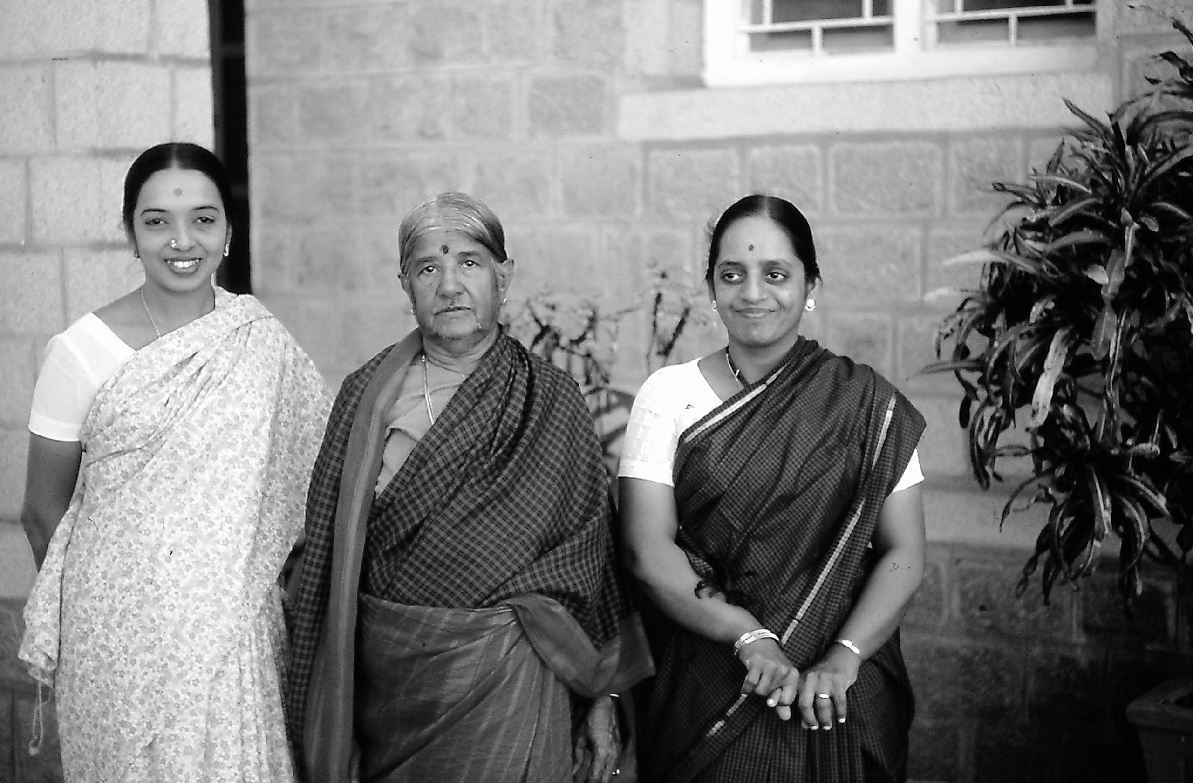
\includegraphics[scale=0.216]{"images/17.jpg"}
\caption{ಕೌಸಲ್ಯ ರಾಮಶೇಷನ್, ಲೋಕಸುಂದರಿ ರಾಮನ್ ಮತ್ತು ಕಮಲ ಜಯರಾಮನ್}\label{chap5-fig01}
\end{figure}

ರಾಮನ್‍ರವರು ತೀರಿಕೊಂಡಾಗ, ಅವರ ಪಾರ್ಥಿವ ಶರೀರವನ್ನು ಪ್ರದರ್ಶನಕ್ಕಿಟ್ಟಿದ್ದ ಹಾಲ್‍ನಿಂದ ಹೊರತೆಗೆಯುವಾಗ ಅವರ ಶ‍್ರೀಮತಿಯವರು ಪಕ್ಕದಲ್ಲಿದ್ದುಕೊಂಡು ಮಗುವಿನಂತೆ ಅತ್ತರು. “ನಾನು ಅವರನ್ನು ಅರವತ್ತು ವರ್ಷಗಳಿಂದ ನೋಡಿಕೊಳ್ಳುತ್ತಿದ್ದೆ. ಈಗ ನೀವು ವಾಪಸಾಗದಂತೆ ಅವರನ್ನು ಕರೆದೊಯ್ಯುತ್ತಿದ್ದೀರಿ” ಎಂದು ಗೋಳಾಡಿದರು. ಒಬ್ಬ ಗಂಭೀರ ವ್ಯಕ್ತಿತ್ವದ ವೃದ್ಧೆಯ ಈ ಅಳಲು ಹೃದಯ ಕಲಕುವಂತಿತ್ತು. ಆಕೆಯು ಈ ಆಘಾತದಿಂದ ಚೇತರಿಸಿಕೊಂಡರು. ಅವರ ಆತ್ಮವಿಶ್ವಾಸವು ಗುರುತರವಾಗಿತ್ತು. ರಾಧಾಕೃಷ್ಣನ್ ಅವರು, ಇನ್ಸಿಟ್ಯೂಟ್ ಡೈರೆಕ್ಟರಾಗಿ ಬೆಂಗಳೂರಿಗೆ ಬಂದಾಗ ಅವರು ಮೊದಲಿನಂತಾದರು. \enginline{1971} ರಿಂದ \enginline{1980}ರ ಅವಧಿಯಲ್ಲಿ ನಾನು ಬೆಂಗಳೂರಿಗೆ ಬಂದಾಗ ಅವರನ್ನು ಭೇಟಿಯಾಗುತ್ತಿದ್ದಾಗ ಬಹಳ ಆತ್ಮೀಯವಾಗಿ ನಡೆದುಕೊಂಡರು. ಲೇಡಿ ರಾಮನ್‍ರವರು ಅನಂತರ ಒಂದು ದಶಕಕ್ಕೂ ಮೀರಿ ಜೀವನ ನಡೆಸಿ \enginline{1980} ಮೇ ತಿಂಗಳಲ್ಲಿ ಕಾಲವಾದರು. ಅವರಿಗೆ ಬೆಂಗಳೂರಿನಲ್ಲಿ ಮೊಮ್ಮಗನ ಜನನವಾದದ್ದೂ, ಮಗ ಡೈರೆಕ್ಟರಾದದ್ದೂ ಬಹಳ ತೃಪ್ತಿ ತಂದ ಸಂಗತಿಗಳಾಗಿದ್ದವು.

\begin{figure}[!htpb]
\centering
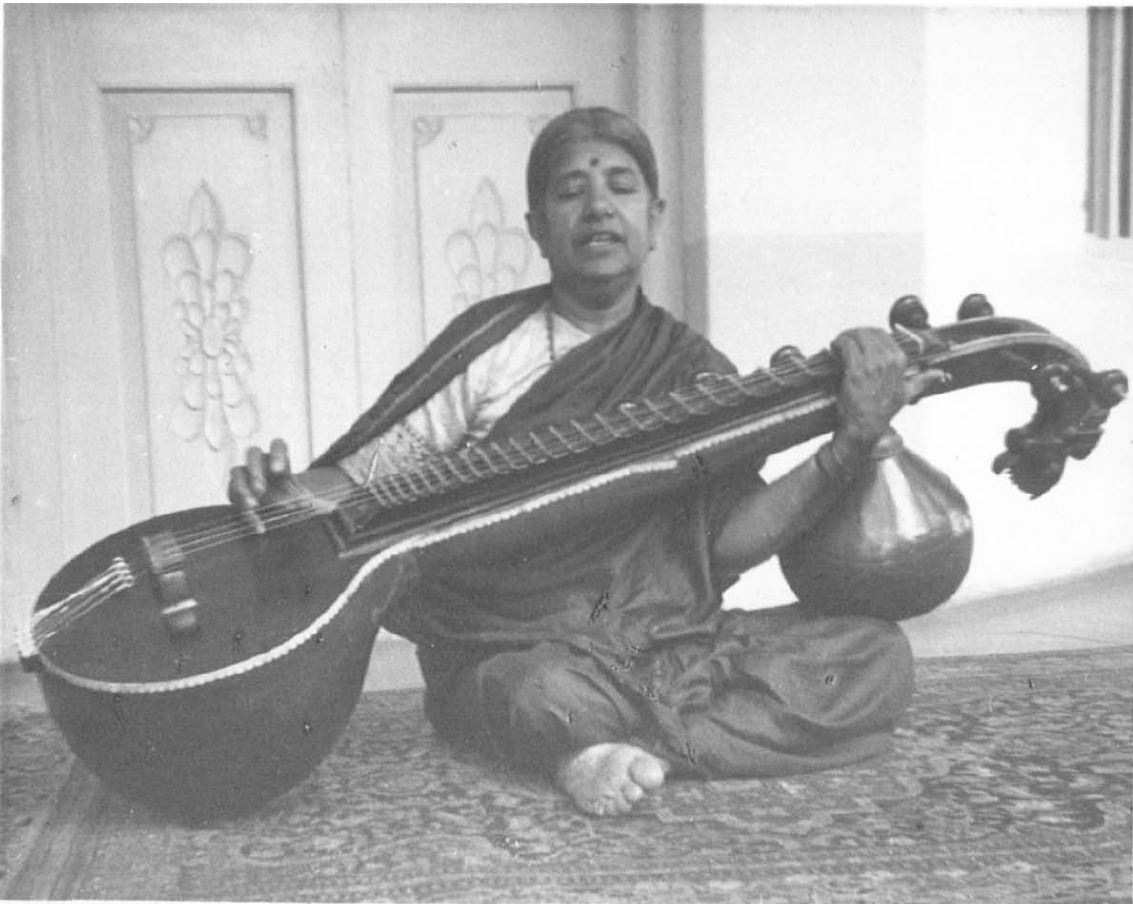
\includegraphics[scale=0.21]{"images/16.jpg"}
\caption{ವೀಣೆ ನುಡಿಸುತ್ತಿರುವ ಲೇಡಿ ರಾಮನ್. ಫೋಟೋ ಕೃಪೆ: ಡೊಮಿನಿಕ್ ರಾಧಾಕೃಷ್ಣನ್}\label{chap5-fig02}
\end{figure}


\heading{ವಿ. ರಾಧಾಕೃಷ್ಣನ್}

ರಾಮನ್ ಅವರ ದ್ವಿತೀಯ ಪುತ್ರ ವಿ. ರಾಧಾಕೃಷ್ಣನ್ ಅವರು ನಮಗೆಲ್ಲಾ ರ‍್ಯಾಡ್ ಆಗಿದ್ದರು. ರಾಮನ್ ಪರಿಣಾಮ ಆವಿಷ್ಕಾರಗೊಂಡ ಕೆಲವು ದಿನಗಳ ಬಳಿಕ \enginline{1929}ರ ಮೇ \enginline{19} ರಂದು ಇವರ ಜನನವಾಯಿತು. ರಾಮನ್ ಇನ್ಸಿಟ್ಯೂಟ್ ಸೇರಿದ ಅನಂತರ ನವೆಂಬರ್ \enginline{1949}ರಲ್ಲಿ ಇವರನ್ನು ನಾನು ಮೊದಲ ಬಾರಿಗೆ ಕಂಡೆ. ಮಲ್ಲೇಶ್ವರಂ ನಲ್ಲಿರುವ ರಾಮನ್ ಅವರ ಬಂಗಲೆ ‘ಪಂಚವಟಿ’ ಯಲ್ಲಿ, ಊಟದ ಮನೆಯ ಕಾರಿಡೋರ್‍ಗೆ ಹೊಂದಿಕೊಂಡಂತೆ ಇದ್ದ ಸಣ್ಣ ಕುಟೀರದಂತಿದ್ದ ಮನೆಯಲ್ಲಿ ಅವರು ವಾಸಿಸುತ್ತಿದ್ದರು.

ಆ ಕುಟೀರದಲ್ಲಿ ಎಲೆಕ್ಟ್ರಾನಿಕ್ಸ್‌ಗೆ ಸಂಬಂಧಿಸಿದ ಅನೇಕ ಪುಸ್ತಕಗಳು ಅಚ್ಚುಕಟ್ಟಾಗಿ ಜೋಡಿಸಿದ್ದವು. ರ‍್ಯಾಡ್ ಅವರಿಗೆ ಎಲೆಕ್ಟ್ರಾನಿಕ್ಸ್‌ನಲ್ಲಿ ವಿಪರೀತ ಆಸಕ್ತಿ. ‘ಅಮೆಚೂರ್ ರೇಡಿಯೋ’ ಮ್ಯಾಗ್‍ಜೀನ್ನ ಎಲ್ಲಾ ಹೊತ್ತಿಗೆಗಳು ಅವರ ಬಳಿ ಇದ್ದವು. ಅಂದಿಗೆ ಅವರು ಸೆಂಟ್ರಲ್ ಕಾಲೇಜಿನಲ್ಲಿ ಭೌತಶಾಸ್ತ್ರದಲ್ಲಿ ಬಿ.ಎಸ್ಸ್ (ಆನರ್ಸ್) ಓದುತ್ತಿದ್ದರು. ರ‍್ಯಾಡ್ ನನ್ನೊಡನೆ ಬಹಳ ಸ್ನೇಹದಿಂದ ಇದ್ದರು. ನಾವಿಬ್ಬರೂ ಅನೇಕ ಬಾರಿ ಭೇಟಿಯಾಗುತ್ತಿದ್ದೆವು. ನಾನು ಅವರಿಂದ ಬಹಳಷ್ಟು ಎಲೆಕ್ಟ್ರಾನಿಕ್ಸ್ ಕಲಿತೆ. ನಾನೂ ಸಹ ಹವ್ಯಾಸಿ ರೇಡಿಯೋ ಫ್ಯಾನ್ ಆಗಿದ್ದೆ. ಇದಲ್ಲದೆ ನನಗೆ ಆಕಾಶದ ತಾರೆಗಳು ಮತ್ತು ರಾಶಿಗಳನ್ನು ಅವರು ಪರಿಚಯಿಸಿದರು. ಇದಕ್ಕಾಗಿ ಊರ ಹೊರಗೆ ಕರೆದೊಯ್ಯುತ್ತಿದ್ದರು. ನಾವು ಪರಸ್ಪರ ಹತ್ತಿರವಾದೆವು. ಬಿ.ಎಸ್ಸಿ ಮುಗಿದ ಬಳಿಕ ಆಗ ಕೆ. ಎಸ್. ಕೃಷ್ಣನ್ ಇದ್ದ ಭೌತಶಾಸ್ತ್ರ ವಿಭಾಗಕ್ಕೆ ಟಾಟಾ ಇನ್ಸ್ಟಿಟ್ಯೂಟ್ ನಲ್ಲಿ ದಾಖಲಾದರು.

ಆದರೆ ಬಹಳ ದಿನ ಅಲ್ಲಿ ವ್ಯಾಸಂಗ ಮಾಡಲಿಲ್ಲ. \enginline{1953}ರ ಸುಮಾರಿಗೆ ಪ್ರೊಫೆಸರ್ ರಿಡ್ ಬೆಕ್ (ಚಾಲ್ಮ್‌ರ್ಸ್ ಇನ್ಸ್ಟಿಟ್ಯೂಟ್ ಆಫ಼್ ಟೆಕ್ನೋಲಜಿ. ಸ್ವೀಡನ್) ಅವರು ಬೆಂಗಳೂರಿಗೆ ಬಂದರು. ಇವರು ರೇಡಿಯೋ ಖಗೋಳವಿಜ್ಞಾನದಲ್ಲಿ ಬಹಳವೇ ತೊಡಗಿಸಿಕೊಂಡಿದ್ದರು. ಇವರು ನಮ್ಮ ರಾಮನ್ ಸಂಸ್ಥೆಗೂ ಭೇಟಿಯಿತ್ತು ಒಳ್ಳೆಯ ಉಪನ್ಯಾಸ ನೀಡಿದ್ದರು. ರಾಧಾಕೃಷ್ಣನ್ ಅವರೂ ರಿಡ್ ಬೆಕ್ ಅವರೂ ಒಳ್ಳೆಯ ಸ್ನೇಹಿತರಾದರು. ಬಹುಶಃ ಇದರಿಂದಲೇ ರ‍್ಯಾಡ್ ಅವರು ರೇಡಿಯೋ ಖಗೋಳವಿಜ್ಞಾನದಲ್ಲಿ ಒಲವು ಬೆಳಸಿಕೊಂಡರು. ಬಹುಶಃ ರಿಡ್ ಬೆಕ್, ರಾಧಾಕೃಷ್ಣನ್ ಅವರಿಗೆ ತಮ್ಮ ಸಂಶೋಧನಾ ತಂಡವನ್ನು ಸೇರಲು ಆಹ್ವಾನಿಸಿದರೆಂದು ತೋರುತ್ತದೆ. ಒಂದು ದಿನ ಇದ್ದಕ್ಕಿದ್ದಂತೆ ರ‍್ಯಾಡ್ ಬೆಂಗಳೂರು ತೊರೆದು ಇಂಗ್ಲೆಂಡ್‍ಗೆ ಹೊರಟರು. ಇದಾದ ಬಳಿಕ ಅವರ ಸಂಪರ್ಕ ನನಗಿಲ್ಲವಾಯಿತು. ಅವರು ರಿಡ್ ಬೆಕ್ ತಂಡವನ್ನು ಯಾವಾಗ ಸೇರಿದರೆಂದು ನನಗೆ ತಿಳಿದಿಲ್ಲ. ಅವರು ಗುರುಗ್ರಹದ ರೇಡಿಯೋ ತರಂಗಗಳ ಬಗ್ಗೆ ಉತ್ತಮವಾದ ಸಂಶೋಧನೆ ಮಾಡಿದರೆಂದು ಕೇಳಿ ಬಲ್ಲೆ.

ನಾನು \enginline{University of California Los Angeles} ಗೆ ಸೇರಿದ ಸ್ವಲ್ಪ ಕಾಲದ ನಂತರ ನನ್ನ ಸ್ನೇಹಿತರಾದ ವೆಂಕಟ ರಾಮನ್, (ಮೆಟೆರೋಲಜಿ ವಿಭಾಗದಲ್ಲಿದ್ದರು) ಇವರು ರ‍್ಯಾಡ್ ಕ್ಯಾಲಿಹೋರ್ನಿಯ ಇನ್ಸ್ಟಿಟ್ಯೂಟ್ ಆಹ್ ಟೆಕ್ನಾಲಜಿ (ಕ್ಯಾಲ್ಟೆಕ್)ಯಲ್ಲಿ ಕೆಲಸ ಮಾಡುತ್ತಿದ್ದಾರೆಂದೂ ಪಸಾಡೆನಾದಲ್ಲಿ ವಾಸವಾಗಿದ್ದಾರೆಂದೂ ತಿಳಿಸಿದರು. ನಾನು ರ‍್ಯಾಡ್ ಅವರನ್ನು ಸಂಪರ್ಕಿಸಿದೆ. ನನ್ನನ್ನು ನೋಡಲು ಬಂದದ್ದೇ ಅಲ್ಲದೆ, ತಮ್ಮ ವಾರಾಂತ್ಯದಲ್ಲಿ ಅಪಾರ್ಟ್‌ಮೆಂಟ್‍ಗೆ ಕರೆದೊಯ್ದರು. ರ‍್ಯಾಡ್ ಅವರಿಗೆ ಭಾರತೀಯ ತಿನಿಸುಗಳು ಇಷ್ಟವಾಗಿದ್ದವು. ಅವರ ಅಪಾರ್ಟ್‌ಮೆಂಟ್ ನಲ್ಲಿ ನನಗೆ ತಿಳಿದಿದ್ದ ದಕ್ಷಿಣ ಭಾರತದ ಪಾಕಶಾಸ್ತ್ರ ಪ್ರಯೋಗಗಳನ್ನು ಮಾಡಿ ಕೊಡುತ್ತಿದ್ದೆ. ಹೀಗೆ ನನಗೆ ಸಲಿಗೆ ಬೆಳೆಯಿತು. ಇನ್ನೊಮ್ಮೆ ನನ್ನನ್ನು ಓವೆನ್ಸ್ ವ್ಯಾಲಿಯಲ್ಲಿದ್ದ ರೇಡಿಯೋ ದೂರದರ್ಶಕ ತೋರಿಸಲು ಕರೆದೊಯ್ದರು. ಅಲ್ಲಿದ್ದ ದೊಡ್ಡಗಾತ್ರದ ರೇಡಿಯೋ ತರಂಗ ಸಂಗ್ರಹಕಗಳನ್ನೂ ಅವುಗಳ ಕಾರ್ಯವಿಧಾನವನ್ನೂ ನಾನಿದ್ದ ಎರಡು ದಿನಗಳಲ್ಲಿ ವಿವರಿಸಿದರು. ಕ್ಯಾಲ್ಟೆಕ್‍ನಲ್ಲಿ ಅವರು ಜಾನ್ ಬೋಲ್ಟನ್ ಅವರ ಸಂಶೋಧನಾ ತಂಡದಲ್ಲಿದ್ದರೆಂದು ನೆನಪು. ಇವರು ಆಸ್ಟ್ರೇಲಿಯದವರು. ಇವರು ತೋರಿಸಿದ್ದನ್ನೆಲ್ಲಾ ಕಂಡು ನಾನು ಪುಳಕಿತನಾದೆ. ಅವರು ಹತ್ತಿರದ ಸಾನ್ ಗಾಬ್ರಿಯೇಲ್ ಪರ್ವತಗಳಿಗೆ ಕರೆದೊಯ್ದಾಗ ನಾನು ಮೊದಲ ಬಾರಿ ಮಂಜು ಬಿದ್ದುದನ್ನು ಕಂಡೆ. ಮಂಜಿನ ಉಂಡೆಗಳನ್ನು ಪರಸ್ಪರ ಎಸೆದು ಮಕ್ಕಳಂತೆ ಖುಷಿಪಟ್ಟೆವು. ಕ್ಯಾಲ್ಟೆಕ್‍ನಲ್ಲೂ ನನ್ನನ್ನು ಓಡಾಡಿಸಿ, ಅಂದಿನ ಕಾಲದ ಪ್ರಸಿದ್ಧ ವಿಜ್ಞಾನಿಗಳನ್ನು ಪರಿಚಯಿಸಿದರು. ನನ್ನ ಪತ್ನಿ ಕಮಲ ಅಮೆರಿಕಾಗೆ ಬಂದ ಮೇಲೆ ವೆಸ್ಟ್ ವುಡ್, ಲೆವೆರಿಂಗ್ ಅವೆನ್ಯೂದಲ್ಲಿ ಮನೆ ಮಾಡಿದಾಗ, ಹಲವಾರು ಬಾರಿ ರ‍್ಯಾಡ್‍ನನ್ನು ಆಹ್ವಾನಿಸಿದ್ದೆವು. ನನ್ನ ಹೆಣ್ಣು ಮಕ್ಕಳನ್ನು ಬಹಳ ಇಷ್ಟಪಟ್ಟಿದ್ದರು. ಹಾಗೆಯೇ ಕಮಲಳು ಮಾಡುವ ಅಡುಗೆಯೂ ಇಷ್ಟವಾಗುತ್ತಿತ್ತು. ನಮ್ಮ ಮಾತುಕತೆಯೆಲ್ಲಾ ತಮಿಳಿನಲ್ಲೇ ಆಗುತ್ತಿತ್ತು.

ಮೈಕ್ರೋವೇವ್ ಆಂಪ್ಲಿಫೈಯರ್ ಬಗ್ಗೆ ಕಲಿಯಲು ಅವರು ನ್ಯೂಜರ್ಸಿಯ ಬೆಲ್ ಲ್ಯಾಬ್‍ಗೆ ಸೇರಿಕೊಂಡರು. ಅಲ್ಲಿ ಡೆರಿಕ್ ಸ್ಕೊವಿಟ್ ಎಂಬುವರು ಈ ರಂಗದಲ್ಲಿ ಪ್ರಸಿದ್ಧರು. ಕ್ಯಾಲ್ಟೆಕ್‍ಗಾಗಿ ಅಂದಿನ ಕಾಲದಲ್ಲಿ ಅತ್ಯುನ್ನತ ತಂತ್ರಜ್ಞಾನ ಒಳಗೊಂಡ ಸೂಕ್ಷ್ಮ ತರಂಗವರ್ಧಕವನ್ನು ಬೆಲ್ ಲ್ಯಾಬ್ಸ್, ಕ್ಯಾಲ್ಟೆಕ್‍ಗಾಗಿ ನಿರ್ಮಿಸಿಕೊಡಲು ಒಪ್ಪಿಕೊಂಡಿತ್ತು. ಡೆರಿಕ್ ಅವರ ತಂಡದಲ್ಲಿ ಸುಮಾರು ಒಂದು ವರ್ಷ ಕೆಲಸಮಾಡಿ, ರ‍್ಯಾಡ್ ತಾವು ಕಲಿತ ವಿದ್ಯೆಯನ್ನು ಓವೆನ್ಸ್ ವ್ಯಾಲಿಯಲ್ಲಿ ಸಾದರಪಡಿಸಿದರು. ಅವರು ಬೆಲ್ ಲ್ಯಾಬ್‍ನಲ್ಲಿ ಇದ್ದಾಗ ನಾನು ಲೇಸರ್‍ಗಳ ಬಗ್ಗೆ ಅತಿ ಕುತೂಹಲದಿಂದ ಇದ್ದೆ. ಬೆಲ್ ಲ್ಯಾಬ್‍ನಲ್ಲಿದ್ದ ಅನೇಕ ಪ್ರಸಿದ್ಧ ವಿಜ್ಞಾನಿಗಳ ಬಗ್ಗೆಯೂ ನನಗೆ ಆಸಕ್ತಿಯಿತ್ತು. ನಾನು ಅವರ ಅಪಾರ್ಟ್‌ಮೆಂಟ್‍ನಲ್ಲಿ ಇದ್ದಾಗ \enginline{University of California Los Angeles} ದಲ್ಲಿನ ನನ್ನ ಕೆಲಸದ ಬಗ್ಗೆಯೂ ಚರ್ಚೆಗಳಾದವು.

ಇದಾದ ಬಳಿಕ \enginline{7–8} ವರ್ಷಗಳ ವರೆಗೆ ನಮ್ಮ ಸಂಪರ್ಕವಿರಲಿಲ್ಲ. ಅವರು ಕ್ಯಾಲ್ಟೆಕ್ ಬಿಟ್ಟು ಆಸ್ಟ್ರೇಲಿಯಾಗೆ ಹೋದರೆಂದೂ, ಅಲ್ಲಿ ರೇಡಿಯೋ ಖಗೋಳವಿಜ್ಞಾನದಲ್ಲಿ ಬಹಳಷ್ಟು ಒಳ್ಳೆಯ ಕೆಲಸಮಾಡಿದರೆಂದೂ ಬಲ್ಲೆ. ಬಹುಶಃ \enginline{1968-69}ರಲ್ಲಿ ಅವರು ತಮ್ಮ ಪತ್ನಿ ಡೊಮಿನಿಕ್ ರವರೊಂದಿಗೆ ಅಮೆರಿಕಾಗೆ ಬಂದರು. ನಾವು ಮುರ್ರೆಹಿಲ್ ನಲ್ಲಿದ್ದಾಗ ನಮ್ಮ ಆತಿಥ್ಯವನ್ನು ಎರಡು ದಿನಗಳ ಮಟ್ಟಿಗೆ ಸ್ವೀಕರಿಸಿದರು. ಅವರು ನಮ್ಮಲ್ಲಿದ್ದಾಗ ಬಹಳ ಸಂತೋಷ ಪಟ್ಟೆವು. ಅವರು ಬಹಳ ಸಿಗರೇಟ್ ಸೇದುತ್ತಿದ್ದದ್ದು ನನಗೆ ಸರಿ ಬೀಳಲಿಲ್ಲ. ಆದರೂ ಅವರಿಗೆ ಹೇಳುವ ಧೈರ್ಯ ಮಾಡಲಿಲ್ಲ.

ಇದರ ಅನಂತರ ನಮ್ಮ ಬೇಟಿಯಾದದ್ದು \enginline{1970}ರಲ್ಲಿ ರಾಮನ್ ಮರಣಿಸಿದಾಗ. ಆಗ ನಾನು ನನ್ನ ಕೆಲಸದಿಂದ ಒಂದು ವರ್ಷದ ಮಟ್ಟಿಗೆ ರಜೆ ಪಡೆದಿದ್ದೆ. ಭಾರತದಲ್ಲಿ ಹೈ ಪ್ರೆಶರ್ ಸಂಶೋಧನೆಗೆ ಬೇಕಾದ ಪ್ರಯೋಗಾಲಯವನ್ನು ಸ್ಥಾಪಿಸಲು ಕೆಲಸಮಾಡುತ್ತಿದ್ದೆ. ರ‍್ಯಾಡ್ ಅವರು, ತಮ್ಮನ್ನು ರಾಮನ್ ಸಂಸ್ಥೆಯ ಭಾರಹೊರಲು, ಒತ್ತಡ ತರುತ್ತಿದ್ದುದ್ದನ್ನು ನನಗೆ ತಿಳಿಸಿದರು. ಭಾರತದಲ್ಲಿನ ವಿಜ್ಞಾನದ ಬೆಳವಣಿಗೆಗೆ ಅವರು ಈ ಹೊರೆ ಹೊತ್ತರೆ ಒಳ್ಳೆಯದಾಗುವುದೆಂದು ನಾನು ಹೇಳಿದೆ. ಕೊನೆಗೂ ಅವರು ರಾಮನ್ ಸಂಶೋಧನ ಸಂಸ್ಥೆಯ ಡೈರೆಕ್ಟರಾಗಲು ಒಪ್ಪಿ, ಬೆಂಗಳೂರಿಗೆ ಬಂದರು. ಎರಡು ದಶಕಗಳವರೆಗೆ ಈ ಸಂಸ್ಥೆಯು ಅವರ ಅಧ್ವರ್ಯುತನದಲ್ಲಿ ಒಳ್ಳೆಯ ಪ್ರಗತಿ ಕಂಡಿತು. ರ‍್ಯಾಡ್ ಒಳ್ಳೆಯ ಸಂಶೋಧನೆಗಳಿಗೆ ಉತ್ತೇಜನ ನೀಡಿ, ಅದರ ಗುಣಮಟ್ಟವನ್ನು ಏರಿಸಿದರು. ಇದರಿಂದ ಅವರಿಗೆ ಭಾರತದಲ್ಲೂ, ಅಂತಾರಾಷ್ಟ್ರೀಯ ಮಟ್ಟದಲ್ಲೂ ಹೆಸರು ಬಂದಿತು.

ರ‍್ಯಾಡ್ ಅವರಿಗೆ ಹಲವಾರು ಹವ್ಯಾಸಗಳಿದ್ದವು. ಅವರು ಹಾರುವ ವಿಮಾನಗಳನ್ನೂ, ಸಾಗರ ಸಂಚಾರಿ ಬೋಟ್ ಗಳನ್ನೂ ನಿರ್ಮಿಸುತ್ತಿದ್ದರು. ನಾನು ಅವರನ್ನು ಭೇಟಿಯಾದಾಗ ಅವರು ನಿರ್ಮಿಸಿದ ಹಾರುವ ಯಂತ್ರವನ್ನು ತೋರಿಸಿದ್ದೇ ಅಲ್ಲದೆ ಇದರಲ್ಲಿ ಅವರಿಗಾದ ಮಾರಣಾಂತಿಕ ಅಪಘಾತದ ಬಗ್ಗೆ ಹಗುರವಾಗಿ ಮಾತನಾಡಿದ್ದರು. ಅವರು ನಿರ್ಮಿಸುತ್ತಿದ್ದ ‘ಕಟಮಾರನ್’ ಬೋಟ್‍ನ ಹಲವಾರು ಅಂಶಗಳನ್ನು ನನಗೆ ವಿವರಿಸಿದ್ದರು. ಅದರಲ್ಲಿ ಆಧುನಿಕ ಸಾಗರ ಸಂಚಾರ ಉಪಕರಣಗಳನ್ನು ಅಳವಡಿಸಿದ್ದರು. ಇದನ್ನು ಕೊಚಿನ್ ಬಳಿಯ ಸಮುದ್ರಕ್ಕೆ ಅವರು ಕೊಂಡೊಯ್ದು ಪ್ರಯಾಣಮಾಡಬೇಕೆಂದಿದ್ದಾಗ ಚಂಡಮಾರುತ ಬಂದು ಅವರು ತಮ್ಮ ಪ್ರಯತ್ನವನ್ನು ಕೈಬಿಡ\-ಬೇಕಾಯಿತಂತೆ.

ಡಿಸೆಂಬರ್ \enginline{2009}ರಲ್ಲಿ ಅವರನ್ನು ಕೊನೆಯ ಬಾರಿ ಕಂಡೆ. ಅವರು ನನ್ನನ್ನು ಮನೆಗೆ ಕರೆದುಕೊಂಡು ಹೋಗಿ ಡೊಮಿನಿಕ್ ತಯಾರಿಸಿದ ಊಟ ಬಡಿಸಿದರು. ಅವರ ಕಛೇರಿಯಲ್ಲಿ ಮಾತನಾಡುತ್ತಿದ್ದಾಗ ನಾನು ರಾಮನ್ ಅವರನ್ನು ನೆನಸಿಕೊಂಡು ಕಣ್ಣೀರಿಟ್ಟಾಗ ನನ್ನನ್ನು ತುಂಬ ಸಮಾಧಾನಪಡಿಸಿದ್ದರು. \enginline{2011} ಮಾರ್ಚ್ \enginline{3} ರಂದು ಅವರು ತೀರಿಕೊಂಡರೆಂದು ಕೇಳಿ ನನಗೆ ಬಹಳ ಸಂಕಟವಾಯಿತು. ನಾನು ಡೊಮಿನಿಕ್ ಅವರಿಗೆ ಸಂತಾಪ ಸೂಚಿಸಿ ಬರೆದ ಪತ್ರಕ್ಕೆ ಆಕೆ ತುಂಬ ವಿನಯದಿಂದ ಉತ್ತರಿಸಿದ್ದರು. ಅವರು ಇಂದಿಗೂ ಅದೇ ಮನೆಯಲ್ಲಿ ವಾಸಿಸುತ್ತಿದ್ದಾರೆ. ಲೇಡಿ ರಾಮನ್ ಅವರ ಜೀವನದಂತೆಯೇ ಇವರ ಜೀವನವೂ ಆಗಿದೆ. ರ‍್ಯಾಡ್ ಅವರು ಹಳೆಯ ಕಾಲದ ವಿಜ್ಞಾನಿಗಳಂತೆಯೇ ಇದ್ದರು. ಬಹಳಷ್ಟು ಸ್ವತಂತ್ರ ಆಲೋಚನೆಯ ವ್ಯಕ್ತಿ. ಯಾರೇ ಬಂದರೂ ಅವರ ಅಂತಸ್ತು ನೋಡದೆ ಆತ್ಮೀಯರಾಗಿರುತ್ತಿದ್ದರು. ಸಂಸ್ಥೆಯಲ್ಲಿದ್ದ ನೌಕರರ ದುಃಖ ದುಮ್ಮಾನಗಳನ್ನು ತಾಳ್ಮೆಯಿಂದ ಕೇಳಿ ಅವರಿಗೆ ನೆರವಾಗುತ್ತಿದ್ದರು. ಅವರು ಎಂದೂ ನ್ಯಾಯಪರವಾಗಿದ್ದರೆಂದು ಕೇಳಿದ್ದೇನೆ. ಇದು ಸತ್ಯವೆಂದೇ ನನಗೆ ಅನಿಸುತ್ತದೆ. ಬುದ್ಧಿವಂತ ವ್ಯಕ್ತಿಗಳೆಂದರೆ ಬಹಳ ಸಂತೋಷಪಟ್ಟು ಹತ್ತಿರಕ್ಕೆ ಕರೆದುಕೊಳ್ಳುತ್ತಿದ್ದರು. ಅವರಿಗೆ ಡಿಗ್ರಿಗಳು ಇದೆಯೇ ಎಂದು ನೋಡುತ್ತಿರಲಿಲ್ಲ. ಅವರೂ ಸಹ ಯಾವುದೇ ಡಿಗ್ರಿ ಪಡೆಯದೇ ಉತ್ತಮ ಸಂಶೋಧಕರಾಗಿ ಮಾದರಿಯಾದರು.

\newpage

\begin{figure}[!htpb]
\centering
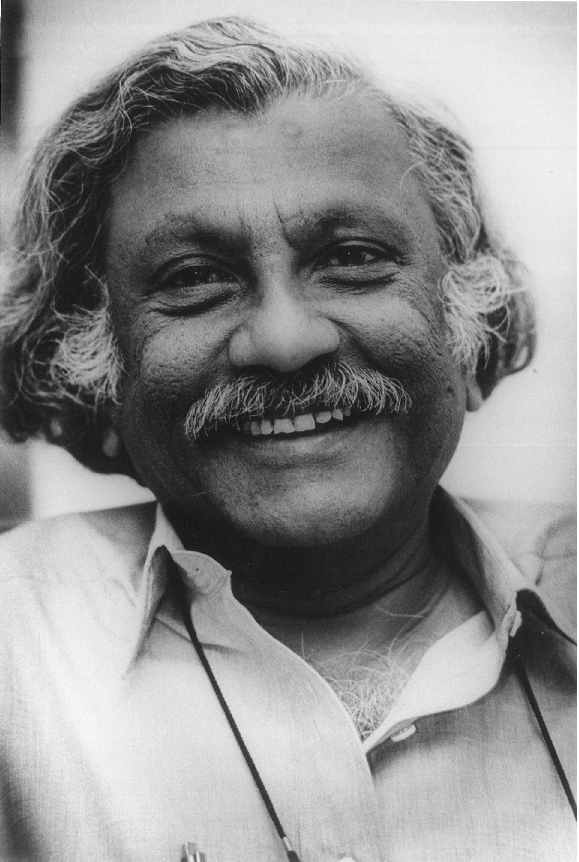
\includegraphics[scale=0.24]{"images/18.jpg"}
\caption{ವಿ. ರಾಧಾಕೃಷ್ಣನ್}\label{chap5-fig03}
\end{figure}


ರ‍್ಯಾಡ್ ಅವರಿಗೆ ತಮ್ಮ ಕ್ಷೇತ್ರದಲ್ಲಿ ಹೆಸರು ಬಂದಿದ್ದು ಅವರ ಉನ್ನತ ಮಟ್ಟದ ಸಂಶೋಧನೆಗಳಿಂದ ಇಂತಹವರು ನನ್ನ ಒಡನಾಡಿಯಾಗಿದ್ದರೆಂಬುದೇ ನನ್ನ ಭಾಗ್ಯ.

\begin{figure}[!htpb]
\centering
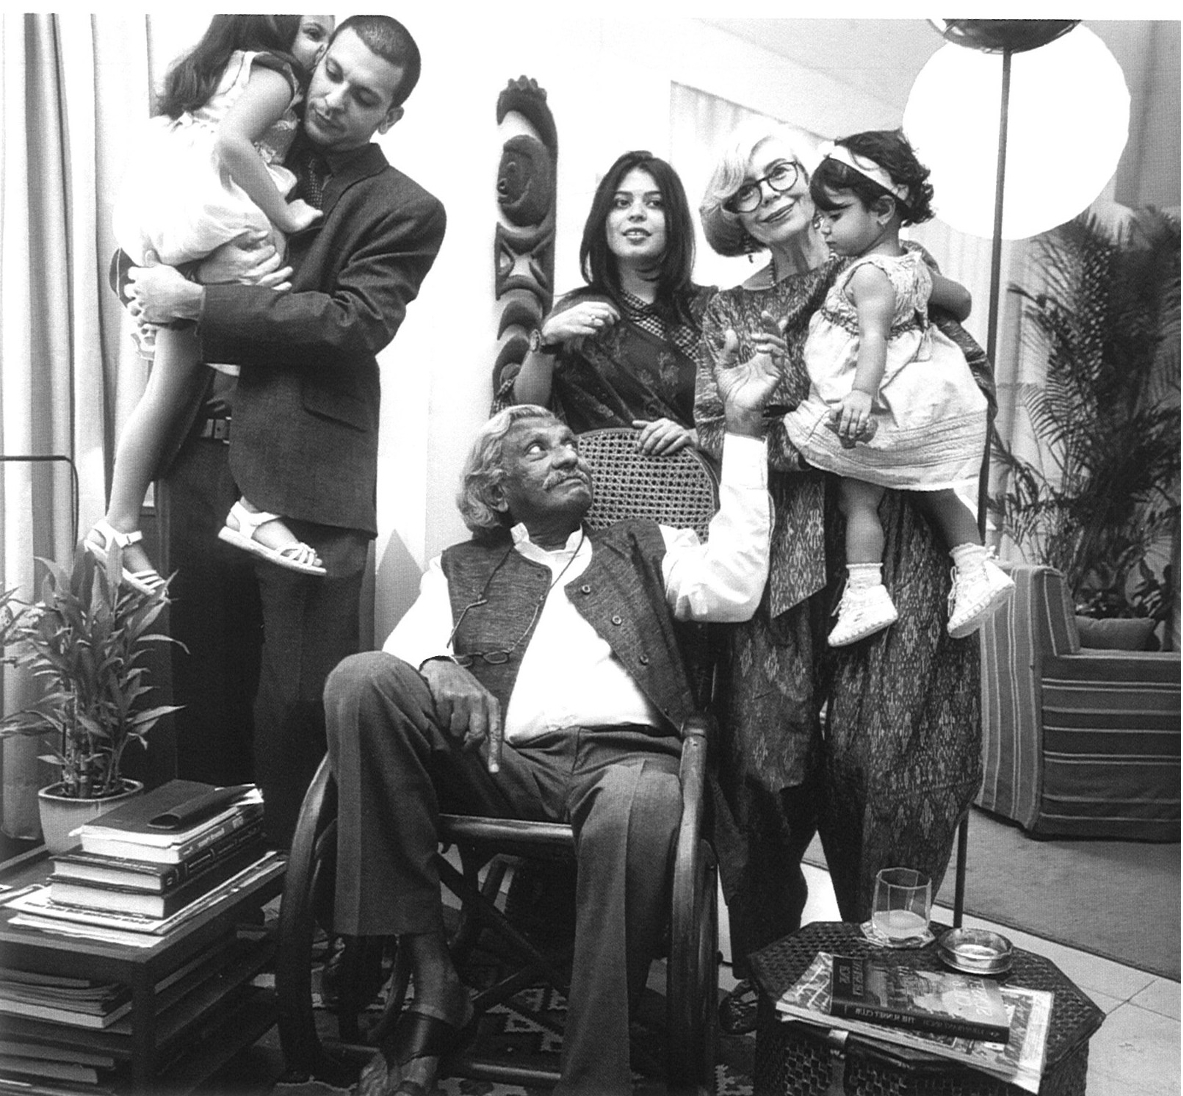
\includegraphics[scale=0.19]{"images/19.jpg"}
\caption{ಕುಟುಂಬದವರೊಡನೆ ರ‍್ಯಾಡ್}\label{chap5-fig04}
\end{figure}


\begin{figure}[!htpb]
\centering
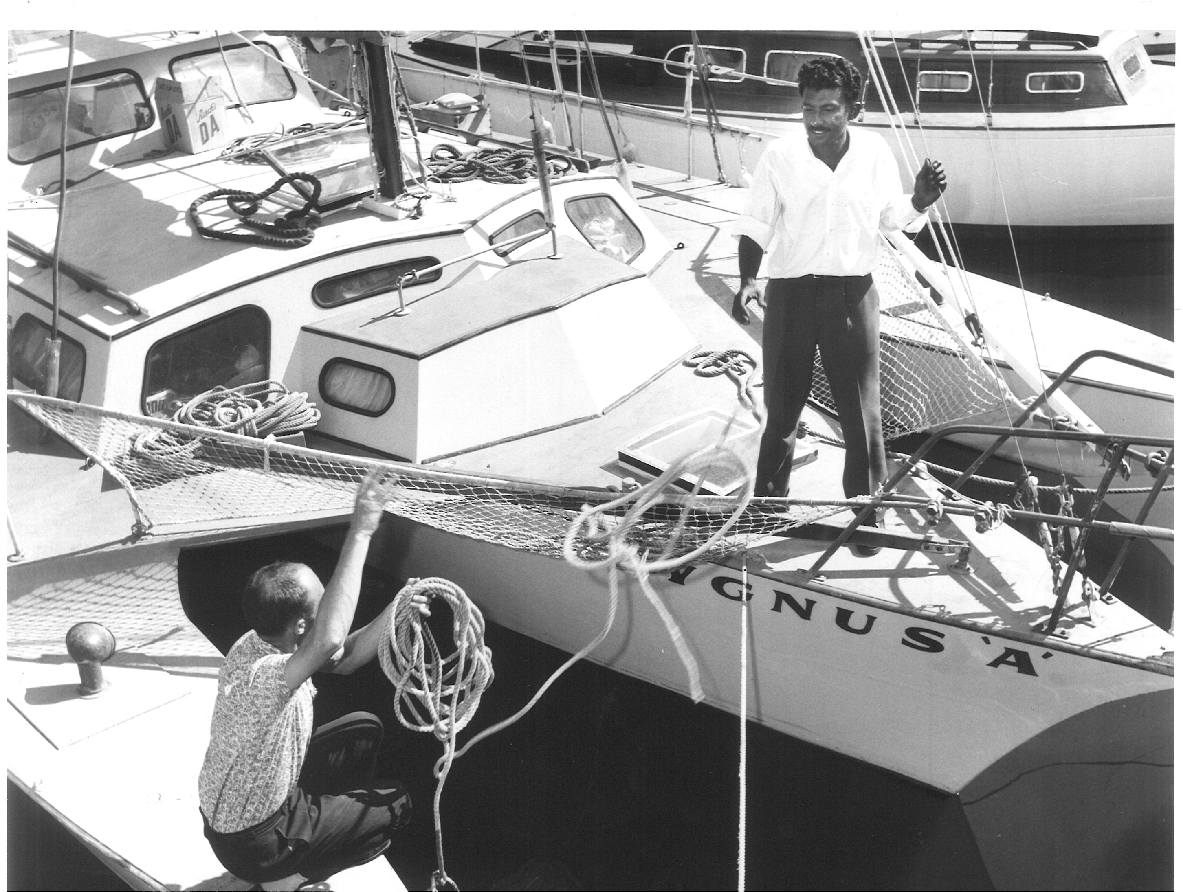
\includegraphics[scale=0.215]{"images/20.jpg"}
\caption{ರ‍್ಯಾಡ್ ಮತ್ತು ಡೇವ್ ರವರ ಜೋಡಿ, ಸಿಡ್ನಿ ಪಟ್ಟಣದಲ್ಲಿ \enginline{1966}}\label{chap5-fig05}
\end{figure}


\begin{figure}[!htpb]
\centering
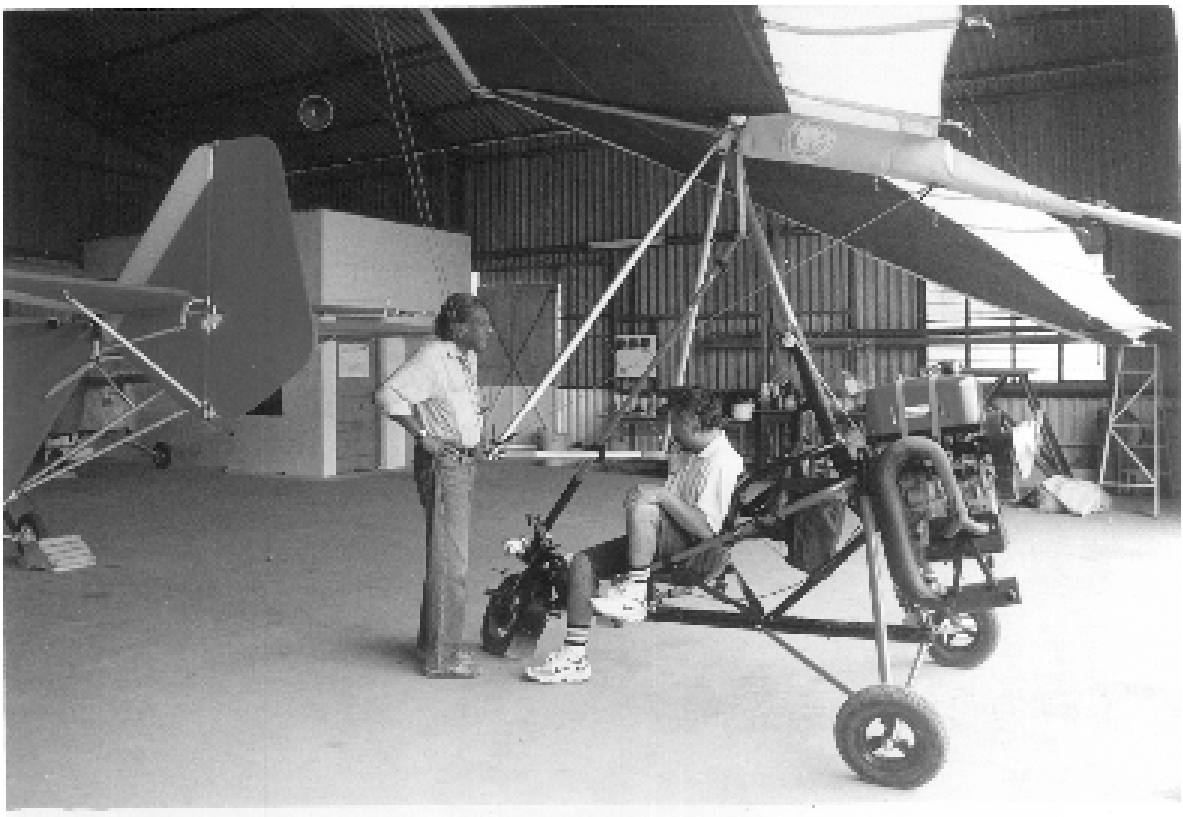
\includegraphics[scale=0.215]{"images/21.jpg"}
\caption{ರ‍್ಯಾಡ್‍ರವರೇ ನಿರ್ಮಿಸಿದ ಗ್ಲೈಡರ್ ಜೊತೆಗೆ. ಫೋಟೋ ಕೃಪೆ: ಡೊಮಿನಿಕ್ ರಾಧಾಕೃಷ್ಣನ್}\label{chap5-fig06}
\end{figure}


\heading{ರಾಮನ್‍ರವರ ಸಂಗೀತಾಸಕ್ತಿ ಮತ್ತು ವಾದ್ಯಗಳು}

ಹೆಲ್ಮ್ ‍ಹೋಲ್ಟ್ಸ್ ಮತ್ತು ರ‍್ಯಾಲೈರವರ ವೈಜ್ಞಾನಿಕ ಕಾರ್ಯಗಳು ರಾಮನ್‍ರವರ ಆಲೋಚನೆ ಮತ್ತು ಸಂಶೋಧನೆಗಳನ್ನು ಬಹಳಷ್ಟು ಪ್ರಭಾವಿಸಿವೆ. ರಾಮನ್‍ರವರು, ಲಾರ್ಡ್ ರ‍್ಯಾಲೈರವರನ್ನು ತಮ್ಮ ಗುರುವೆಂದೇ ಸ್ವೀಕರಿಸಿದ್ದರು. ಅವರು ತಮ್ಮ ಗುರುವನ್ನು ಎಂದೂ ಸಂಧಿಸಿರಲಿಲ್ಲ. ಈ ಇಬ್ಬರು ಹಿರಿಯ ವಿಜ್ಞಾನಿಗಳು ಧ್ವನಿಯ ಬಗ್ಗೆ ಉತ್ತಮ ಗ್ರಂಥಗಳನ್ನು ರಚಿಸಿದ್ದರು. ತಮ್ಮ ವಿದ್ಯಾರ್ಥಿ ದೆಸೆಯಲ್ಲಿಯೇ ರಾಮನ್‍ರವರು ಈ ಗ್ರಂಥಗಳನ್ನು ಓದಿದ್ದರು. ಇದರಿಂದ ಸ್ಫೂರ್ತಿಗೊಂಡು ಇಂಡಿಯನ್ ಅಸೋಸಿಯೇಷನ್ ಫಾರ್ ಕಲ್ಟಿವೇಶನ್ ಆಫ಼್ ಸೈನ್ಸ್‌ನಲ್ಲಿ ಅವನ್ನೇ ಮತ್ತೆ ಓದಿ, ಧ್ವನಿ ವಿಜ್ಞಾನದಲ್ಲಿ ಸಂಶೋಧನೆ ಶುರು ಮಾಡಿದರು. ಧ್ವನಿ ವಿಜ್ಞಾನದಲ್ಲಿ ಭಾರತೀಯ ವಾದ್ಯಗಳ ಬಗ್ಗೆ ಅವರು ಗಾಢ ಆಸಕ್ತಿ ವಹಿಸಿದರು.

ಸಂಗೀತ ಮತ್ತು ಗಣಿತಗಳು ಅನೇಕ ಸಮಾನ ಅಂಶಗಳುಳ್ಳವು. ಇವೆರಡೂ ಮಾನವ ಬುದ್ಧಿ ಶಕ್ತಿಯಿಂದ ಸೃಜಿಸಿದವು. ಆದರೂ ಸಂಗೀತಜ್ಞನಾಗಲಿ ಅಥವಾ ಗಣಿತಜ್ಞನಾಗಲಿ ತನ್ನ ಕ್ಷೇತ್ರ ಬಿಟ್ಟು ಬೇರೆ ಕ್ಷೇತ್ರದಲ್ಲಿ ತಲೆ ಹಾಯಿಸಲಿಲ್ಲ. ಇದಕ್ಕೆ ಅಪವಾದವೆಂದರೆ ಪೈಥಾಗೊರಸ್ ಒಬ್ಬನೇ. ಇವೆರಡೂ ರಂಗಗಳಲ್ಲಿ ಸಿದ್ಧಿ ಪಡೆದು ಮಾನವನ ಕಿವಿಗೆ ಸಂಗೀತವೆಂದರೆ ಯಾವ ಧ್ವನಿ ಎಂದು ಸಂಶೋಧಿಸಿದವನು. ಮೀಟಿದ ತಂತಿಯ ಕಂಪನಗಳ ಶ್ರುತಿ/ಸ್ಥಾಯಿಯು, ತಂತಿಯ ಉದ್ದವನ್ನು ಅರ್ಧಕ್ಕೆ ಇಟ್ಟು ಮೀಟಿದಾಗ, ಒಂದು ಆಕ್ಟೇವ್‍ನಷ್ಟು ಹೆಚ್ಚಾಗುತ್ತದೆ. ಇದನ್ನು ಆಧಾರವಾಗಿಟ್ಟುಕೊಂಡು ಸ್ವರ ಮೇಳದ ಸಿದ್ಧಾಂತವನ್ನು ಬೆಳೆಸಿದರು. ಒಂದು ತಂತಿಯನ್ನು ಮೀಟಿದಾಗ ಮೂಲ ಆವೃತ್ತಿಯಲ್ಲಿನ ಕಂಪನವಷ್ಟೇ ಅಲ್ಲದೆ, ಇತರೆ ಉನ್ನತ ಸ್ವರಗಳನ್ನೂ ಹೊರಡಿಸುತ್ತದೆ. ಒಳ್ಳೆಯ ಸಂಗೀತವಾಗುವುದು ಈ ಅನುಸ್ವರಗಳು \enginline{1:2:3} ಅನುಪಾತದಲ್ಲಿದ್ದಾಗ. ಈ ಅನುಸ್ವರಗಳೇ ಮಾನವನ ಕಿವಿಗೆ ಇಂಪಾಗಿ ಕೇಳಿಸುತ್ತವೆ.

ಪಿಟೀಲಿನಂತಹ ತಂತಿ ವಾದ್ಯಗಳಲ್ಲಿ, ದಾರದ ಕಮಾನಿನಿಂದ ಕಂಪನ ಹೊರಡಿಸಲಾಗುತ್ತದೆ. ಇಂತಹ ವಾದ್ಯಗಳ ಸಿದ್ಧಾಂತದ ಬಗ್ಗೆ ರಾಮನ್‍ರವರು ತಮ್ಮ ಸಂಶೋಧನೆಗೆ ಮೊದಲಿಟ್ಟರು. ತಂತಿಗಳ ಕಂಪನಗಳ ಬಗ್ಗೆ ಗಣಿತಜ್ಞರಿಗೂ, ಭೌತಶಾಸ್ತ್ರಜ್ಞರಿಗೂ ತೀವ್ರ ಆಸಕ್ತಿ. ಇದರಲ್ಲಿ ಹುಟ್ಟುವ ಸಮಸ್ಯೆಗಳು ಇಬ್ಬರಿಗೂ ಅಪ್ಯಾಯಮಾನ. ಅಲ್ಲದೆ ಸ್ವರಗಳ ಮೇಳವೂ ಅತಿ ಸುಂದರ. ತಂತಿಯೊಂದನ್ನು ಎಳೆದು ಎರಡು ಗೂಟಗಳ ನಡುವೆ ಕಟ್ಟಿ, ಅದರಲ್ಲುಂಟಾಗುವ ಸರಳ ರೇಖಾತ್ಮಕ ಕಂಪನಗಳ ಸಿದ್ಧಾಂತವು ಚೆನ್ನಾಗಿಯೇ ಬೆಳವಣಿಗೆಯಾಗಿತ್ತು. ಆದರೂ ಪಿಟೀಲಿನಂತಹ ತಂತಿ ವಾದ್ಯದಲ್ಲಿ ಸೃಜಿಸಬಹುದಾದ ಸ್ವರ ಮೇಳವುಂಟಾಗುವುದಾದರೂ ಹೇಗೆಂದು ತಿಳಿದಿರಲಿಲ್ಲ. ಆಗಿನ ಕಾಲಕ್ಕೆ ಸ್ಟ್ರಾಡಿವೇರಿಯಸ್ ನಂತಹ ಉತ್ತಮ ಪಿಟೀಲುಗಳಿದ್ದವು. ಪಿಟೀಲು ಸ್ವರ ಮೇಳಗಳ ನಿಯಮಗಳೂ ಸಹ ನಿಗೂಢವಾಗಿದ್ದವು. ರಾಮನ್‍ರವರು ಕೈಗೊಂಡ ಸಂಶೋಧನೆಗಳಲ್ಲಿ, ಪಿಟೀಲಿನ ಕಮಾನು ತಂತಿಯನ್ನು ಸ್ಪರ್ಶಿಸುವ ಬಿಂದುವಿನ ಚಲನೆ ಮತ್ತು ತಂತಿಯನ್ನು ಬಿಗಿದು ಕಟ್ಟಿದಾಗ ಪಿಟೀಲಿನ ಕಾಯಭಾಗಕ್ಕೆ (\enginline{Body}) ಸಂಬಂಧ ಬೆಸೆಯುವ “ಕುದುರೆ” ಗಳು ಪ್ರಧಾನ ಪಾತ್ರವಹಿಸುತ್ತವೆಂದು ತಿಳಿದು ಬಂದಿತು.

\newpage 

ರಾಮನ್‍ರವರು ಚರ್ಮವಾದ್ಯಗಳ ಮೇಲೆ ಮಾಡಿದ ಪ್ರಯೋಗಗಳು ಅತಿ ಮುಖ್ಯವಾದವು. ಚರ್ಮವಾದ್ಯಗಳು ಅತಿ ಪ್ರಾಚೀನ ಕಾಲದಿಂದ ಬಂದವುಗಳು. ಜಗತ್ತಿನಾದ್ಯಂತ ಅನೇಕ ಬಗೆಯ ಚರ್ಮ\-ವಾದ್ಯಗಳು ಕಂಡು ಬರುತ್ತವೆ. ಭಾರತದಲ್ಲಿ ಅನಾದಿ ಕಾಲದಿಂದಲೂ ತಬಲಾ ಮತ್ತು ಮೃದಂಗಗಳು ಬಳಕೆಯಲ್ಲಿವೆ. ಇವು ಬಹಳ ವಿಶಿಷ್ಟವಾದವು. ಏಕೆಂದರೆ ಎಲ್ಲ ಬಗೆಯ ಚರ್ಮ ವಾದ್ಯಗಳಲ್ಲಿ ಸಂಗತಿಗಳ ಸುತ್ತಮುತ್ತ ಇರುವ ಅನುಸ್ವರಗಳನ್ನು ಹೊರಡಿಸುವ ವಾದ್ಯಗಳು ಇವೆರಡೆ. ಮಿಕ್ಕೆಲ್ಲ ಚರ್ಮ ವಾದ್ಯಗಳಾವುವೂ ಅಂಶಸ್ವರಗಳನ್ನು ಹೊರಡಿಸಲಾರವು. ಅಂದರೆ ಇವೆಲ್ಲ ಶಬ್ದ ಹೊರಡಿಸುತ್ತವೆ ಅಷ್ಟೆ, ನಾದವನ್ನಲ್ಲ. ರಾಮನ್‍ರವರು ಭಾರತೀಯ ಸಂಗೀತ ವಾದ್ಯಗಳ ವೈಶಿಷ್ಟ್ಯವನ್ನು ಗಮನಿಸಿದರು. ಇದರ ಭೌತಶಾಸ್ತ್ರ ಕಾರಣಗಳ ಬಗ್ಗೆ ಅವರ ಕುತೂಹಲವು ಇಮ್ಮಡಿಗೊಂಡಿತು. ತಬಲ ಮತ್ತು ಮೃದಂಗಗಳು ಸಂಗತಿಗಳ ಸುತ್ತ ಇರುವ ಅಂಶ ಸ್ವರಗಳನ್ನು ಹೊರಡಿಸುತ್ತವೆಂದು ತಿಳಿಸಿಕೊಟ್ಟರು. ಇದು ಸಾಧ್ಯವಾಗುವುದು ಇವುಗಳ ಚರ್ಮ ಹೊದಿಕೆಯ ಕೇಂದ್ರದಲ್ಲಿ ಮೆತ್ತಿದ ಮೆದು ಹಿಟ್ಟಿನಿಂದ. ಈ ಮೆದುವಾದ ಹಿಟ್ಟು ಅಂಟಾಗಿಯೂ, ಮೆತ್ತಗೂ ಇರುತ್ತದೆ. ಚರ್ಮದ ಮೇಲೆ ಹಿಟ್ಟು ಮೆತ್ತಿರುವುದರಿಂದ, ಚರ್ಮದ ಮೇಲೆ ಏಟು ಬಿದ್ದಾಗ ಉಂಟಾಗುವ ಅನುಸ್ವರಗಳು, ಇದೇ ಚರ್ಮದ ವಿಭಿನ್ನ ಕಂಪನ ಆವೃತ್ತಿಗಳಲ್ಲಿ ಇರುತ್ತವೆ ಎಂಬ ಅಂಶವು ಸಂಶೋಧನೆಯಲ್ಲಿ ಹೊರಬಿದ್ದಿತು. ತಬಲ/ಮೃದಂಗವನ್ನು ಬೆರಳುಗಳಲ್ಲಿ ತಾಡಿಸಿ ರಾಮನ್‍ರವರು ಈ ಎಲ್ಲಾ ಬಗೆಯ ಕಂಪನ ಆವೃತ್ತಿಗಳನ್ನು ಕೆಲ ನಿರ್ದಿಷ್ಟ ಬಿಂದುಗಳ ಮೇಲೆ ಬೆರಳುಗಳಲ್ಲಿ ಬಡಿದು ಪ್ರಾತ್ಯಕ್ಷಿಸಿಕೊಂಡರು. ಅವರು ಮೊದಲ ಬಾರಿಗೆ ಅನುಸ್ವರಗಳಿರುತ್ತವೆಂದು ಕಂಡುಕೊಂಡಾಗ ಈಗಿನಂತೆ ಆಂದೋಲಕಗಳು ಇರಲಿಲ್ಲ. ವಿದ್ಯುನ್ಮಾನ ವಿಶ್ಲೇಷಕಗಳೂ ಇರಲಿಲ್ಲ. ಅವರಿಗಿದ್ದದ್ದು ಅವರ ಸೂಕ್ಷ್ಮ ಕಿವಿಯೊಂದೇ. ರಾಮನ್‍ರವರು ಚರ್ಮವಾದ್ಯಗಳಲ್ಲಿ ಈ ಅಂಶಸ್ವರಗಳನ್ನು ಕಾಣಲು ಮೃದಂಗ/ತಬಲಗಳ ಚರ್ಮದ ಮೇಲೆ ಲೈಕೋಪೋಡಿಯಂನ ಧೂಳನ್ನು ಹಾಕಿದ್ದರು. ಚರ್ಮ ತಾಡನ ಮಾಡಿದಾಗ ಅದರ ಮೇಲೆ ಧೂಳಿನಲ್ಲಿ ಉಂಟಾಗುವ ತರಂಗ ವಿನ್ಯಾಸಗಳನ್ನು ಗಮನಿಸಿ ತಮ್ಮೆಲ್ಲಾ ಸಂಶೋಧನೆಗಳನ್ನು ಮಾಡಿದ್ದರು.

ದಶಕಗಳುರುಳಿದನಂತರ ಚರ್ಮ ವಾದ್ಯಗಳ ಮೇಲಿನ ಸಂಶೋಧನೆಯನ್ನು ಪ್ರೊಫೆಸರ್\break ರಾಮಕೃಷ್ಣರವರು ಟಾಟಾ ವಿಜ್ಞಾನ ಸಂಸ್ಥೆಯಲ್ಲಿ ಮುಂದುವರೆಸಿದರು. ಚರ್ಮವನ್ನು ವಿವಿಧ ಆಧುನಿಕ ತಂತ್ರಜ್ಞಾನ ಉಪಕರಣಗಳಿಂದ ಉತ್ತೇಜಿಸಿ, ರಾಮನ್‍ರವರ ಎಲ್ಲಾ ಆವಿಷ್ಕಾರಗಳನ್ನು ನಿಜವೆಂದು ಸಾಬೀತು ಪಡಿಸಿದರು. ರಾಮಕೃಷ್ಣನ್ ಮತ್ತು ತಂಡದವರು ಇದನ್ನು ಸಮಗ್ರವಾಗಿ ಸಂಶೋಧನೆಗೈದು ವಿಷಯ ಮಂಡನೆ ಮಾಡಿದ್ದಾರೆ.

ವೀಣೆ ಮತ್ತು ತಂಬೂರಿಗಳನ್ನು ಭಾರತದಲ್ಲಿ ದೈವದತ್ತವೆಂದೇ ಬಗೆದಿದ್ದಾರೆ. ಇವುಗಳ ನಾದದ ಇಂಪು ಕಿವಿಗೆ ಬಲುಹಿತ. ಧ್ವನಿಶಾಸ್ತ್ರದ ಪ್ರಕಾರ ಹೊರಡಿಸಲಾಗದ ಅನೇಕ ಅಂಶಸ್ವರಗಳು ಈ ಎರಡು ತಂತಿ ವಾದ್ಯಗಳನ್ನು ಮೀಟಿದಾಗ ತೀವ್ರವಾಗಿ ಹೊರಡಿಸುತ್ತವೆಂಬುದನ್ನು ರಾಮನ್‍ರವರು ಸಂಶೋಧಿಸಿದರು. ಇದು ಯಂಗ್\enginline{--}ಹೆಲ್ಮ್‌ಹೋಲ್ಟ್ಸ್ ನಿಯಮವನ್ನು ಮೀರಿದಂತೆ ಆಗುತ್ತದೆ. ಎರಡೂ ವಾದ್ಯಗಳಲ್ಲಿ ಈ ಪರಿಣಾಮವುಂಟಾಗುವುದು ಕಮಾನಿನಂತಹ “ಕುದುರೆ” ಯಿಂದಾಗಿ. ಇದನ್ನು ಭಾರತದಲ್ಲಿನ ಸಂಗೀತಜ್ಞರು ಅನೇಕ ಪ್ರಯೋಗಗಳನ್ನು ಮಾಡಿ, ತಿಳಿದುಕೊಂಡಿದ್ದರು. ಹೀಗೆ ವೀಣೆ ಮತ್ತು ತಂಬೂರಿಗಳು ಹೆಚ್ಚಿನ ಗುಣಮಟ್ಟದ ಶಬ್ದ ತರಂಗಗಳನ್ನು ಹೊರಡಿಸಬಲ್ಲವು. ಹಾಡುಗಾರಿಕೆಗೆ ತಂಬೂರಿಯಿಲ್ಲದಿದ್ದರೆ ಸಾಧ್ಯವೇ ಇಲ್ಲ. ಹಿಮ್ಮೇಳದ ಶ್ರುತಿಗಾಗಿ ತಂಬೂರಿ ಇರಲೇ ಬೇಕು.

ರಾಮನ್‍ರವರ ಧ್ವನಿಶಾಸ್ತ್ರದ ಅಧ್ಯಯನಗಳು ಭಾರತೀಯ ವಾದ್ಯಗಳಿಗಷ್ಟೆ ಸೀಮಿತವಾಗಿರಲಿಲ್ಲ. ಪಶ್ಚಿಮದ ಸಂಗೀತಕ್ಕೂ ಅದು ಹರಡಿತ್ತು. ನಾವು ಪಿಟೀಲಿನ ಬಗ್ಗೆ ಅವರ ಸಂಶೋಧನೆಗಳನ್ನು ವಿವರಿಸಿದ್ದೇವೆ. ಪಿಯಾನೋ ವಾದ್ಯಗಳಲ್ಲಿನ ಸುತ್ತಿಗೆಯ ಏಟು ಹೇಗೆ ನಾದ ಉಂಟು ಮಾಡುತ್ತದೆ ಮತ್ತು ವಿಶೇಷವಾಗಿ ವೂಲ್ಫ್‌ನೋಟ್ ಎಂದು ಕರೆಯುವ ಸ್ವರವು ಚಲ್ಲೋ ಮತ್ತು ಪಿಟೀಲುಗಳಲ್ಲಿ ಮಾತ್ರ ಹೊರಡಿಸಲು ಹೇಗೆ ಸಾಧ್ಯ ಎಂಬುದು ಅಭಿಜಾತ ಸಂಶೋಧನೆಗಳು, ಮತ್ತು ಇದಕ್ಕೆ ರಾಮನ್‍ರವರು ನೀಡಿದ ಗಣಿತ ಸಿದ್ಧಾಂತದ ಮಾದರಿಗಳು ಜಗತ್ತಿನಾದ್ಯಂತ ಪ್ರಸಿದ್ಧಿ ಪಡೆದವು. ಸಂಗೀತ ಕ್ಷೇತ್ರದಲ್ಲಿ ರಾಮನ್‍ರವರ ಅಭಿಜಾತ ಕಾರ್ಯಕ್ಕೆ ಮನ್ನಣೆ ನೀಡಿ, \textit{\general{\enginline{Handbuch der Physik}}} ಎಂಬ ಪ್ರಸಿದ್ಧ ವಿಶ್ವಕೋಶಕ್ಕಾಗಿ ಧ್ವನಿಶಾಸ್ತ್ರ ಸಂಬಂಧಿ ಪ್ರಬಂಧಗಳನ್ನು ಬರೆದುಕೊಡಲು ವಿನಂತಿಸಲಾಯಿತು. ಅರವತ್ತರ ದಶಕದಲ್ಲಿ \enginline{Catgut Acoustical Sty in America} ಸಂಸ್ಥೆಯು (ಪಿಟೀಲಿನ ಧ್ವನಿಶಾಸ್ತ್ರಕ್ಕೆ ಮೀಸಲಾದ ಸಂಸ್ಥೆ). ರಾಮನ್‍ರನ್ನು ಗೌರವ ಸದಸ್ಯರಾಗಿ ಚುನಾಯಿಸಿತು.

ರಾಮನ್‍ರವರು ಸಂಗೀತವನ್ನು ವೈಜ್ಞಾನಿಕ ಸಂಶೋಧನೆಗಳಿಗೆ ಮಾತ್ರ ಬಳಸಿಕೊಳ್ಳಲಿಲ್ಲ. ಅವರಿಗೆ ದಕ್ಷಿಣಾದಿ ಸಂಗೀತ ಬರುತ್ತಿತ್ತು. ಅವರು ಪಿಟೀಲು ವಾದಕರೂ ಆಗಿದ್ದರೂ. ಲೇಡಿ ರಾಮನ್‍ರವರು ವೀಣಾ ವಿದುಷಿಯಾಗಿದ್ದರು. ಅವರನ್ನು ಬೆಂಗಳೂರಿನ ಗಾಯನ ಸಭೆಗಳಲ್ಲಿ ಹಲವಾರು ಬಾರಿ ಕಂಡಿದ್ದೇನೆ. ನಾನೂ ಸಹ ಅವರನ್ನು ಇಂತಹ ಸಭೆಗಳಿಗೆ ಕರೆದೊಯ್ದಿದ್ದೇನೆ. ಆದರೆ ರಾಮನ್‍ರವರನ್ನು ಸಂಗೀತ ಸಭೆಗಳಲ್ಲಿ ನಾನು ಕಂಡಿಲ್ಲ. ಒಮ್ಮೆ ಯಾರದೋ ಮದುವೆಯ ರಿಸೆಪ್‍ಶನ್‍ನಲ್ಲಿ ಎಂ. ಎಸ್. ಸುಬ್ಬಲಕ್ಷ್ಮಿ ಯವರ ಸಂಗೀತ ಕಛೇರಿಯಿತ್ತು. ರಾಮನ್‍ರವರು ತಮ್ಮ ಕಾರನ್ನು ಈ ಮದುವೆ ಮಂಟಪದ ಹೊರಗೆ ನಿಲ್ಲಿಸುವಂತೆ ಚಾಲಕರಿಗೆ ಹೇಳಿದರು. ಸುಮಾರು \enginline{15} ನಿಮಿಷಗಳ ಕಾಲ ಸುಬ್ಬಲಕ್ಷ್ಮಿಯವರ ಸಂಗೀತ ಆನಂದಿಸಿದರು. ಬಳಿಕ ಹೊರಡಲು ಹೇಳಿ ನನ್ನ ಕಡೆ ತಿರುಗಿ\enginline{--}“ನೋಡಯ್ಯ ಸುಬ್ಬಲಕ್ಷ್ಮಿಯ ಕಂಠ ಹೇಗೆ ಬದಲಾಗಿದೆ, ನಿನ್ನ ಅರಿವಿಗೆ ಬಂತೇ” ಎಂದರು. ನಾನೂ ಹೌದು ಎಂದೆ. ಸುಬ್ಬಲಕ್ಷ್ಮಿಯವರು ಸಿನಿಮಾಗಳಿಗೆ ಹಾಡುತ್ತಿದ್ದ ಶೈಲಿ ಬದಲಾಗಿ, ಈಗ ಪೂರ್ಣವಾಗಿ ಸಂಗೀತ ವಿದುಷಿಯಾಗಿ ಹೊರಹೊಮ್ಮಿದ್ದರು.

ಅರವತ್ತರ ದಶಕದಲ್ಲಿ ಒಮ್ಮೊಮ್ಮೆ ತಾತಾಚಾರ್ ಎಂಬ ವಯೋಲಿನ್ ವಾದಕರನ್ನು ಮನೆಗೆ ಕರೆಸು\-ತ್ತಿದ್ದರು. ಲೇಡಿ ರಾಮನ್‍ರವರು, ತಮ್ಮ ಪತಿಗಾಗಿ ಸಂಗೀತ ಕಛೇರಿ ಏರ್ಪಡಿಸುತ್ತಿದ್ದರು.

ರಾಮನ್‍ರವರ ಅಣ್ಣಂದಿರಾದ ಸಿ.ಸುಬ್ರಮಣ್ಯ ಅಯ್ಯರ್ ಪ್ರಸಿದ್ಧ ಪಿಟೀಲು ವಿದ್ವಾಂಸರಾಗಿದ್ದರು. ಅವರು \textit{\general{\enginline{Grammar of South Indian Carnatic Music}}} ಎಂಬ ಪುಸ್ತಕ ಬರೆದಿದ್ದಾರೆ. ಇದರಲ್ಲಿ ಕರ್ನಾಟಕ ಸಂಗೀತದ ರಾಗ ಮೇಳಗಳ ಬಗ್ಗೆಯೂ, ಸ್ವರಗಳ ಬಗ್ಗೆಯೂ, ಸುಸ್ವರ ರಾಗಗಳಲ್ಲಿನ ತರಂಗ ಆವರ್ತಗಳ ಬಗ್ಗೆಯೂ ಬರೆದಿದ್ದಾರೆ. ಇದು ಕರ್ನಾಟಕ ಸಂಗೀತ ಸಿದ್ಧಾಂತ ಪರಿಚಯಿಸುವ ಅತ್ಯುತ್ತಮ ಗ್ರಂಥ. ಮದ್ರಾಸ್ ಮ್ಯೂಸಿಕ್ ಅಕಾಡೆಮಿಯ ತಾಂತ್ರಿಕ ಸಭೆಗಳ ಜವಾಬ್ದಾರಿಯು ರಾಮನ್‍ರವರ ಅಣ್ಣ, ಸಿ. ಎಸ್. ಅಯ್ಯರ್‍ರವರದಾಗಿತ್ತು. ಈ ಅಕಾಡೆಮಿಯು ಡಿಸೆಂಬರ್‍ನ ಕೊನೆಯ ಎರಡು ವಾರಗಳಲ್ಲಿ ತನ್ನ ಸಂಗೀತ ಕಾರ್ಯಕ್ರಮಗಳನ್ನು ನಡೆಸುತ್ತದೆ. ಸಂಗೀತದ ಅತಿ ಸೂಕ್ಷ್ಮ ವಿಚಾರಗಳ ಬಗ್ಗೆಯೂ ಅಲ್ಲಿ ಚರ್ಚಾಕೂಟಗಳಿರುತ್ತವೆ.

\newpage

ರಾಮನ್‍ರವರ ಕುಟುಂಬದಲ್ಲಿ ಸಂಗೀತದ ಎಳೆ ಹರಿಯುತ್ತಿತ್ತು. ಹೀಗಾಗಿ ರಾಮನ್‍ರವರಿಗೆ ಸಹಜವಾಗಿ ಸಂಗೀತಾಸಕ್ತಿ ಮತ್ತು ಸೆಳೆತಗಳಿದ್ದವು. ಇವೇ ರಾಮನ್‍ರನ್ನು ಸಂಗೀತ ವಾದ್ಯಗಳ ವೈಜ್ಞಾನಿಕ ವಿಶ್ಲೇಷಣೆಗೆ ಪ್ರೇರೇಪಿಸಿ ಅದರಲ್ಲಿ ಅತಿ ಶ್ರೇಷ್ಠ ಸಂಶೋಧನೆಗಳಿಗೆ ಪ್ರೇರಣೆಯಾಯಿತು.


\heading{ರಾಮನ್ ಪರಿಣಾಮ}

ಜನಸಾಮಾನ್ಯರಿಗೆ ರಾಮನ್ ಪರಿಣಾಮವನ್ನು ವಿವರಿಸುವುದು ಸುಲಭವಲ್ಲ. ವಿಜ್ಞಾನದಲ್ಲಿ ಉನ್ನತ ವ್ಯಾಸಂಗ ಮಾಡಿದವರಿಗೆ ಮಾತ್ರ ಇದು ಅರ್ಥವಾದೀತು. ಆದರೆ ರಾಮನ್‍ರವರು ತಮ್ಮ ಆವಿಷ್ಕಾರವನ್ನು ಕುರಿತು \textit{“\general{\enginline{A New Radiation}}”} “ಇದೊಂದು ಹೊಸ ವಿಕಿರಣ” ಎಂಬ ಶೀರ್ಷಿಕೆಯಡಿಯಲ್ಲಿ ಜಗತ್ತಿಗೆ ತಿಳಿಸಿದ ಉಪನ್ಯಾಸವು ಅದರ ಸರಳತೆಗೂ, ಸ್ಪಷ್ಟತೆಗೂ ಜ್ವಲಂತ ಉದಾಹರಣೆಯಾಗಬಲ್ಲುದು. ಚಾರಿತ್ರಿಕವಾಗಿ ಇದು ಬಹಳ ಮುಖ್ಯ ಉಪನ್ಯಾಸವಾಗಿದೆ. ನಾನು ಓದುಗರಿಗಾಗಿ ಇದನ್ನು ಯಥಾವತ್ತಾಗಿ ಇಲ್ಲಿ ಉದ್ಧರಿಸಿದ್ದೇನೆ.

ಒಮ್ಮೆ ಹೈಸ್ಕೂಲು ವಿದ್ಯಾರ್ಥಿಗಳ ಗುಂಪೊಂದು ತಮಿಳುನಾಡಿನಿಂದ ರಾಮನ್ ಸಂಸ್ಥೆ ನೋಡಲು ಬಂದಿತ್ತು. ಇಬ್ಬರು ಉಪಾಧ್ಯಾಯರು \enginline{30} ಮಕ್ಕಳನ್ನು ಕರೆ ತಂದಿದ್ದರು. ರಾಮನ್‍ರವರು ಇವರನ್ನೆಲ್ಲಾ ತಮ್ಮ ಸ್ಪಟಿಕಗಳ ಸಂಗ್ರಹವನ್ನು ತೋರಿಸಲು ಕರೆದೊಯ್ದರು. ವಿವರಣೆಗಾಗಿ ಅಲ್ಲಲ್ಲಿ ತಮಿಳನ್ನೂ ಬಳಸಿಕೊಂಡರು. ಆ ವಿದ್ಯಾರ್ಥಿಗಳು ನಮಗೆ ರಾಮನ್ ಪರಿಣಾಮವನ್ನು ತಮಿಳಿನಲ್ಲಿ ಹೇಳಬೇಕೆಂದು ಬೇಡಿದರು. ರಾಮನ್‍ರವರು ಈ ಗುಂಪನ್ನು ಉಪನ್ಯಾಸ ಕೊಠಡಿಯಲ್ಲಿ ಕೂಡಿಸಿ ತಮಿಳಿನಲ್ಲಿ ಮಾತನಾಡತೊಡಗಿದರು. ನಾನು ಅಲ್ಲಿ ಹೋಗಿ ಕುಳಿತೆ. ಇವರು ತಮಿಳಿನಲ್ಲಿ ಹೇಗೆ ವಿವರಿಸುವರೆಂಬ ಕುತೂಹಲವೂ ಇತ್ತು. ಅವರು ತಮಿಳಿನಲ್ಲಿ ಹೇಳಿದ್ದು ಹೀಗೆ

\enginline{--}ಟೆನ್ನಿಸ್ ಕೋರ್ಟ್‌ನಲ್ಲಿ ಚೆಂಡನ್ನು ಆಚೀಚೆ ಬ್ಯಾಟಿನಿಂದ ಹೊಡೆಯುವುದನ್ನು ಜ್ಞಾಪಿಸಿಕೊಳ್ಳಿ. ಬ್ಯಾಟ್ ಅನ್ನು ಹಿಂದಿನಿಂದ ಮುಂದಕ್ಕೆ ಬೀಸಿ ಚೆಂಡನ್ನು ಹೊಡೆಯ ಬೇಕಷ್ಟೆ. ಈ ಕಡೆಯಿಂದ ಚೆಂಡು ಆ ಕಡೆಗೆ ಹೋಗಿದೆಯೆಂದು ಇಟ್ಟುಕೊಳ್ಳಿ. ಹೀಗೆ ಎದುರಿನಲ್ಲಿರುವ ಕೋರ್ಟ್‌ಗೆ ನುಗ್ಗಿದ ಚೆಂಡು, ಅಲ್ಲಿ ಬೀಸುವ ಬ್ಯಾಟನ್ನು ತಾಗಬೇಕು. ಆ ಬ್ಯಾಟ್ ಚೆಂಡು ಚಲಿಸುವ ದಿಕ್ಕಿನಲ್ಲೇ, ಹಿಂದಕ್ಕೆ ಚಲಿಸಿದ್ದಾದರೆ, ಬ್ಯಾಟಿನಿಂದ ಪುಟಿಯುವ ಚೆಂಡು ತನ್ನ ಕೊಂಚ ವೇಗವನ್ನು ಕಳೆದು ಕೊಳ್ಳುತ್ತದೆ ಮತ್ತು ಹಿಂದಕ್ಕೆ ವಾಪಸ್ ಬರುತ್ತದೆ. ಆದರೇ ಇದೇ ಚೆಂಡು ಮುನ್ನುಗ್ಗಿದಾಗ ಬ್ಯಾಟು ಮುಂದಕ್ಕೆ ಚಲಿಸಿ ಚೆಂಡನ್ನು ಘಟ್ಟಿಸಿದರೆ, ಬ್ಯಾಟಿನ ವೇಗವು ಚೆಂಡಿಗೆ ದಾಟಿ ಅದು ಹಿಂದಕ್ಕೆ ಪುಟಿಯುವ ವೇಗ ಹೆಚ್ಚಾಗುತ್ತದೆ. ಅಂದರೆ ಅದನ್ನು ಎಸೆದಾಗಿನ ವೇಗಕ್ಕಿಂತಲೂ, ವಾಪಸ್ ಬರುವ ವೇಗ ಹೆಚ್ಚು.

ರಾಮನ್ ಪರಿಣಾಮವು ಬೆಳಕು, ಮತ್ತು ಅಣುಗಳ ನಡುವೆ ನಡೆಯುತ್ತದೆ. ನೀವು ಆಪಾತ ಬೆಳಕನ್ನು, ಒಳಗೆಸೆದ ಚೆಂಡಿನಂತೆ ಭಾವಿಸಿ, ಅಣುಗಳು ಈ ಬೆಳಕನ್ನು ಘಟ್ಟಿಸಿ ಪುಟಿಸುತ್ತವೆ. ಅಣುವಿನಲ್ಲಿ, ಪರಮಾಣುಗಳು ನಿರಂತರವಾಗಿ ಕಂಪಿಸುತ್ತಿರುತ್ತವೆ. ಈ ಕಂಪನವು ಸಮಬಲ ಕೇಂದ್ರದ ಆಚೀಚೆ ಉಂಟಾಗುತ್ತಿರುತ್ತದೆ. ಬೆಳಕಿಗೂ ಸಹ ಕಂಪನವಿದೆ. ತರಂಗಾಂತರವೂ ಇದೆ. ಅದು ಏಕವರ್ಣೀಯವಾಗಿದ್ದಾಗ ಬೆಳಕಿನ ಕಣವು, ಅಣುವಿಗೆ ಘಟ್ಟಿಸಿದಾಗ, ಬೆಳಕಿನ ಆವರ್ತವು ಹೆಚ್ಚಾಗಬಹುದು ಅಥವಾ ಕಡಿಮೆಯಾಗಬಹುದು. ಇದು ಅಣುವಿನ ಶಕ್ತಿ ಸಂಗ್ರಹದ ಮೇಲೆ ಅವಲಂಬಿತವಾಗಿರುತ್ತದೆ. ಅಣುವು ಶಕ್ತಿಯನ್ನು ದಾಟಿಸಿದಾಗ ಬೆಳಕಿನ ಆವರ್ತವು ಜಾಸ್ತಿ ಯಾಗುವುದು, ಅದರ ಆವರ್ತವು ಕಡಿಮೆಯಾಗುವುದು \enginline{—} ಅಣುವು ಶಕ್ತಿಯನ್ನು ಹೀರಿಕೊಂಡಾಗ ಟೆನ್ನಿಸ್ ಚೆಂಡು ಬ್ಯಾಟಿನಿಂದ ವೇಗ ಪಡೆಯುವುದೂ, ವೇಗ ತಗ್ಗಿಸಿಕೊಳ್ಳುವುದೂ ಇದ್ದಂತೆ.

ಇದನ್ನು ವಿದ್ಯಾರ್ಥಿಗಳು ಅರ್ಥ ಮಾಡಿಕೊಂಡರೋ ಇಲ್ಲವೋ ನಾ ಕಾಣೆ. ಆದರೆ ಇದು ಅತ್ಯಂತ ಸಮಂಜಸ ಉದಾಹರಣೆ.


\heading[ಒಂದು ಹೊಸ ವಿಕಿರಣ]{ಒಂದು ಹೊಸ ವಿಕಿರಣ\protect\footnotemark[1]}
\footnotetext[1]{ಬೆಂಗಳೂರಿನಲ್ಲಿ \enginline{1928}ರ ಮಾರ್ಚ್ \enginline{16}, ಶುಕ್ರವಾರದಂದು ದಕ್ಷಿಣ ಭಾರತೀಯ ವಿಜ್ಞಾನ ಸಂಘದ ಉದ್ಘಾಟನ ಭಾಷಣವನ್ನು ಮಾಡಿದರು, ಹಾಗು ಅದೇ ವಿಚಾರವನ್ನು \enginline{\textit{Indian Journal of Physics}, 1928, Vol. 2, pp. 387–398} ನಲ್ಲಿ ಪ್ರಕಟವಾಗಿದೆ.}

\noindent
\textbf{ಪೀಠಿಕೆ:}

ಅಣು ಮತ್ತು ಪರಮಾಣುಗಳಿಂದ ಹೊರ ಸೂಸುವ ಬೆಳಕಿನ ಹೊಸಬಗೆಯ ಕಿರಣಗಳ ಬಗ್ಗೆ ಇಂದಿನ ಸಂಜೆ ಮಾತನಾಡಲು ಉದ್ದೇಶಿಸಿದ್ದೇನೆ. ಇದರ ಗಹನತೆಯನ್ನು ಮನದಟ್ಟು ಮಾಡಲು, ನಾವು ಕಲ್ಕತ್ತದಲ್ಲಿ ಕೈಗೊಂಡ ಪ್ರಯೋಗಗಳ ಚರಿತ್ರೆಯನ್ನು ಒಂದಿಷ್ಟು ಹೇಳಬೇಕು. ಇವೇ ನಮ್ಮನ್ನು ಈ ಹೊಚ್ಚ ಹೊಸ ಸಂಶೋಧನೆಗೆ ಹಾದಿ ತೋರಿಸಿದವು. ಇವನ್ನು ನಿಮ್ಮ ಮುಂದಿಡುವ ಮುನ್ನ ಅಣುಗಳು ಮತ್ತು ಪರಮಾಣುಗಳಿಂದ ಉಂಟಾಗುವ ವಿಕಿರಣಗಳ ಬಗ್ಗೆ ಒಂದಿಷ್ಟು ಮಾಹಿತಿ ನೀಡಿದರೆ ಇಲ್ಲಿ ವಿಷಯಾಂತರವಾಗಲಾರದು.

ಅಣುಗಳು ಮತ್ತು ಪರಮಾಣುಗಳು ಬೆಳಕು ಸೂಸುವ ಹಲವಾರು ಬಗೆಗಳು ಭೌತವಿಜ್ಞಾನಿಗಳಿಗೆ ತಿಳಿದಿವೆ. ಉದಾಹರಣೆಗೆ ವಸ್ತುವೊಂದನ್ನು ಬಿಸಿ ಮಾಡಿದಾಗ ಅಥವಾ ವಸ್ತುವಿಗೆ ಎಲೆಕ್ಟ್ರಾನುಗಳ ಪ್ರವಾಹವೊಂದನ್ನು ತಾಡಿಸಿದಾಗ ಅಣು ಮತ್ತು ಪರಮಾಣುಗಳು ಬೆಳಕನ್ನು ಹೊರ ಚೆಲ್ಲುತ್ತವೆ. ಹೀಗೆ ಹೊರಬಿದ್ದ ಬೆಳಕು ಆಯಾ ಅಣು, ಪರಮಾಣುಗಳ ಗುಣ ಲಕ್ಷಣಗಳಿಗೆ ಹೊಂದಿಕೊಂಡಿರುತ್ತವೆ. ಇದಕ್ಕೆ ಪ್ರೈಮರಿ (ಪ್ರಾಥಮಿಕ) ವಿಕಿರಣಗಳು ಎನ್ನುತ್ತಾರೆ. ಅತಿ ಹೆಚ್ಚು ಬೆಳಕಿಗೆ ಅಣು/ಪರಮಾಣುಗಳನ್ನು ಒಡ್ಡಿದಾಗಲೂ, ಅವುಗಳಿಂದ ಬೆಳಕು ಹೊರಡುವಂತೆ ಮಾಡಬಹುದು. ಇಂತಹ ಬೆಳಕಿಗೆ ಸೆಕೆಂಡರಿ (ದ್ವಿತೀಯಕ) ವಿಕಿರಣಗಳು ಎನ್ನುತ್ತಾರೆ. ಎಲ್ಲರಿಗೂ ಗೊತ್ತಿರುವ ವಿಸರಣ (ಪ್ರಕ್ರಿಯೆಯು) ದ್ವಿತೀಯಕ ವಿಕಿರಣಗಳಿಗೆ ಉದಾಹಣೆಯಾಗಬಲ್ಲುದು. ಆದರೆ ಇದು ಹೆಸರಿಗೆ ಮಾತ್ರ. ಇಂತಹವನ್ನು ವಸ್ತುವಿನ ಮೇಲ್ಮೈಯಲ್ಲಿ ಉಂಟಾಗುವ ಪ್ರತಿಫಲನಗಳ ಪ್ರಕ್ರಿಯೆಯಾಗಿಯೂ ಪರಿಗಣಿಸಬಹುದು. ಏಕೆಂದರೆ ವಸ್ತುವಿನ ಅಣುಗಳು ಅಥವಾ ಪರಮಾಣುಗಳು ಇಂತಹ ದ್ವಿತೀಯಕ ವಿಕಿರಣ ಸೂಸುವಿಕೆಯಲ್ಲಿ ಪಾಲ್ಗೊಳ್ಳುವುದೇ ಇಲ್ಲ. ದ್ವಿತೀಯಕ ನೈಜ ವಿಕಿರಣಗಳನ್ನು ಕಂಡು ಹಿಡಿದವನು ಸ್ಟೋಕ್ಸ್ ಎಂಬ ವಿಜ್ಞಾನಿ. ಇವನು ಕಂಡು ಹಿಡಿದ ಪ್ರಕ್ರಿಯೆಯನ್ನು ಪ್ರತಿದೀಪ್ತಿ (\enginline{Florascence}) ಎನ್ನುತ್ತಾರೆ. ಸ್ಟೋಕ್ಸ್ ಕೆಲವು ನಿಯಮಗಳನ್ನೂ ಈ ಪರಿಣಾಮಕ್ಕೆ ನಿರೂಪಿಸಿದ್ದಾನೆ. ಹಲವಾರು ಸಾವಯವ ಬಣ್ಣಗಳು ಈ ಪರಿಣಾಮವನ್ನು ಚೆನ್ನಾಗಿ ತೋರಿಸುತ್ತವೆ. ನಾನು ಇಲ್ಲೊಂದು ನೀರಿನ ಬಾಟಲಿಯನ್ನಿರಿಸಿದ್ದೇನೆ. ಬಹಳ ಅಲ್ಪ ಪ್ರಮಾಣದಲ್ಲಿ ಸಂಯುಕ್ತ ವಸ್ತು ಫ್ಲೋರೆಸೀನ್ ಸೇರಿಸಿದ್ದೇನೆ. ಇದನ್ನು ಲಾಂಟ್ರೆನ್‍ನ ಬೆಳಕಿನಲ್ಲಿ ಇರಿಸಿದ್ದಾದರೆ, ಈ ನೀರು ಹಸಿರು ಬಣ್ಣದಿಂದ ಹೊಳೆಯುತ್ತಿದೆ. ಆಪಾತ ಬೆಳಕಿನಲ್ಲಿ ಫಿಲ್ಟರ್‌ಗಳನ್ನು ಇಟ್ಟು, ಬೇಕಾದ ಬಣ್ಣದ ಬೆಳಕು ಹಾಯಿಸಿದಾಗ ತಿಳಿದು ಬರುವ ಅಂಶವೆಂದರೆ, ಬಾಟಲಿನಿಂದ ಹೊರಬೀಳುವ ಬೆಳಕಿನ ಬಣ್ಣ ಬದಲಾಗುವುದಿಲ್ಲ. ನೇರಳೆ ಬಣ್ಣವು, ಹಸಿರು ಬಣ್ಣದ ಪ್ರಖರತೆಯನ್ನು ಹೆಚ್ಚು ಮಾಡುತ್ತದೆ. ಕೆಂಪು ಬಣ್ಣವು ಇದನ್ನುಂಟುಮಾಡುವುದಿಲ್ಲ. ಅಂದರೆ ಬೆಳಕಿನ ಪ್ರಖರತೆ ಬದಲಾಗಬಹುದು, ಬಣ್ಣವಲ್ಲ.

ಇನ್ನೊಂದು ಬಗೆಯ ದ್ವಿತೀಯಕ ವಿಕಿರಣ ಪ್ರಕ್ರಿಯೆ ಇದೆ. ಅದು ಬೆಳಕಿನ ಚದರುವಿಕೆಯಿಂದ ಉಂಟಾಗುವಂತಹುದು. ಇದನ್ನು ಇತ್ತೀಚೆಗೆ ಪ್ರಯೋಗಗಳಿಂದ ಧೃಢಪಡಿಸಿಕೊಳ್ಳಲಾಗಿದೆ. ಆಕಾಶದ ನೀಲಿ ಬಣ್ಣ, ಆಳ ಸಾಗರದ ನೀಲಿ, ಹಾಗೆಯೇ ಶುದ್ಧ ಮಂಜುಗಡ್ಡೆಯ ಅಪಾರಕತೆಗಳು (\enginline{Opalascence}) ಈ ಬಗೆಯ ಬೆಳಕಿನ ಚದರುವಿಕೆಯಿಂದ ಉಂಟಾದವುಗಳು. ನನ್ನ ಬಳಿ ಇರುವ ಈ ದೊಡ್ಡ ಬಾಟಲಿಯಲ್ಲಿ ಟೌಲೀನ್ ದ್ರವವಿದೆ. ಇದು ಯಾವುದೇ ಬೆರಕೆಯಿಲ್ಲದ ಶುದ್ಧ ಪಾರದರ್ಶಕ ದ್ರವ. ಆದರೂ ಇದರ ಮೂಲಕ ಹಾಯಿಸಿದ ಬೆಳಕು ಅದರ ಪಥವನ್ನು (ಶಂಕುವಿನಾಕಾರದಲ್ಲಿ) ಹೊಳಪು ನೀಲಿ ಬಣ್ಣದಿಂದ ತೋರಿಸುತ್ತಿದೆ.

ಟೌಲೀನ್ ದ್ರವವನ್ನು ಅದೆಷ್ಟೇ ಬಾರಿ ಶುದ್ಧ ಮಾಡಿದರೂ ಸಹ ಈ ಬಣ್ಣ ಕಂಡೇ ಕಾಣುತ್ತದೆ. ಇದೇ ಬಗೆಯ ಚದರುಬಣ್ಣವು ಅನಿಲಗಳಲ್ಲೂ, ಆವಿಗಳಲ್ಲೂ ಮತ್ತು ಘನವಸ್ತುಗಳಲ್ಲೂ ಕ್ಷೀಣವಾಗಿಯಾದರೂ ಕಂಡು ಬರುತ್ತದೆ. ಒಂದು ದೊಡ್ಡ ಪಾರದರ್ಶಕ ಮಂಜುಗಡ್ಡೆಯ ಮೂಲಕ ಸೂರ್ಯನ ಬೆಳಕನ್ನು ಹಾಯಿಸಿದಾಗ, ಆ ಬೆಳಕಿನ ಪಥವು ನೀಲಿ ಬೆಳಕನ್ನು ಸೂಸುತ್ತದೆ. ಆಪ್ಟಿಕಲ್ ಗಾಜಿನ ಖಂಡಗಳನ್ನು ಪೇರಿಸಿಟ್ಟಾಗ ಉಂಟಾಗುವ ಚದರ ನೀಲಿ ಬೆಳಕಿನ ಪ್ರಕಿಯೆಯನ್ನು ಇದೇ ಬಗೆಯಲ್ಲಿ ತೋರಿಸಬಹುದು. ಹೀಗೆ ಅಣುಗಳಿಂದ ಬೆಳಕಿನ ಚದರುವಿಕೆಯು ಉಂಟಾಗುವುದು ವಸ್ತುಗಳ ಸಾಮಾನ್ಯ ಲಕ್ಷಣವಾಗಿದೆ.

ಕಲ್ಕತ್ತದಲ್ಲಿ ಕಳೆದ ಏಳು ವರ್ಷಗಳಿಂದ, ಪಾರದರ್ಶಕ ವಸ್ತುಗಳಲ್ಲಿ ಚದರುವ ಬೆಳಕಿನ ಬಗ್ಗೆ, ತೀವ್ರವಾದ ಸಂಶೋಧನೆಗಳು ನಡೆಯುತ್ತಿವೆ. ಹೊಸ ಪ್ರಯೋಗಗಳೂ, ಸಿದ್ಧಾಂತಗಳೂ ಹೊರ\-ಬರುತ್ತಿವೆ. ಇದರದ್ದೇ ಮುಂದುವರಿಕೆಯ ಸರಣಿಯಲ್ಲಿ  ನಾನಿಲ್ಲಿ ಹೇಳ ಹೊರಟಿರುವ ಆವಿಷ್ಕಾರವಾಗಿದೆ. ನಮ್ಮ ಸಂಶೋಧನೆಗಳಿಂದ ಹೊರಬಿದ್ದ ಅಂಶವೆಂದರೆ, ವಸ್ತುಗಳಲ್ಲಿ ಬಿಳಿ ಬೆಳಕಿನ ಚದರುವಿಕೆಯು ಅಣುಗಳಿಂದ ಉಂಟಾಗುತ್ತದೆ ಎಂಬುದು ಮೊದಲನೆಯದು. ಎರಡನೆಯದಾಗಿ ಇಡೀ ಪರಿಣಾಮ\-ವನ್ನು ಉಷ್ಣಮೂಲ ಅಂಶಗಳಿಂದಲೂ ವಿವರಿಸಬಹುದು. ಉಷ್ಣದಿಂದಾಗಿ ಅಣುಗಳು ಕಂಪಿಸ\-ತೊಡಗುತ್ತವೆ, ಮತ್ತು ಅವುಗಳ ಜೋಡಣೆಯು ಅಸ್ತವ್ಯಸ್ತವಾಗುತ್ತದೆ. ಇದರಲ್ಲಿ ಯಾವುದೇ ವಿನ್ಯಾಸವಿರುವುದಿಲ್ಲ. ಹೀಗಾದಾಗ ಉಂಟಾಗುವ ದ್ಯುತಿವಿಭಿನ್ನತೆ (\enginline{heterogenity}) ಮತ್ತು ಇದರ ಪರಿಣಾಮವಾಗಿ ಬೆಳಕಿನ ವಿಸರಣ ಉಂಟಾಗುವುದು. ಹೀಗೆ ಬೆಳಕಿನ ಚದರುವಿಕೆಯು ಅಣು ಭೌತವಿಜ್ಞಾನ, ಉಷ್ಣಗತಿ ಶಾಸ್ತ್ರ ಮತ್ತು ವಿಕಿರಣಗಳ ತರಂಗ ಸಿದ್ಧಾಂತಗಳ ಮೇಳದಿಂದಾಗಿ ಹಲವಾರು ಪರಿಣಾಮಗಳ ಊಹೆಗೆ ಅವಕಾಶ ಮಾಡಿಕೊಟ್ಟು, ಅವುಗಳನ್ನು ಪ್ರಾಯೋಗಿಕವಾಗಿ ಸಾಬೀತು ಪಡಿಸಿಕೊಳ್ಳುವುದು ಆಧುನಿಕ ಭೌತವಿಜ್ಞಾನದ ಗೆಲುವು ಎನ್ನಿಸುತ್ತದೆ.


\heading{ನವೀನ ಪರಿಣಾಮ}

ಕಲ್ಕತ್ತದಲ್ಲಿ ನಡೆಸಿದ ಪ್ರಯೋಗಗಳ ಅಂಕಿಅಂಶಗಳು ಉಷ್ಣಗತಿಶಾಸ್ತ್ರ ತರಂಗ ಸಿದ್ಧಾಂತಗಳ ಅಡಿಯಲ್ಲಿ ಬೆಳಕಿನ ಚದರುವಿಕೆಗಳು ಸೂಚಿಸುವುದನ್ನು ಧೃಡೀಕರಿಸಿದವು. ಆದರೂ ಕೆಲವು ಹೊಸ ಪರಿಣಾಮಗಳು ನಮ್ಮ ಪೂರ್ವ ತಿಳುವಳಿಕೆಗಳಿಗಿಂತ ಬೇರೆಯಾಗಿದ್ದವು. ನಮ್ಮ ಪೂರ್ವ\break
 ತಿಳುವಳಿಕೆಗಳಿಗೂ, ಹೊಸ ಪರಿಣಾಮದ ಪ್ರಾಯೋಗಿಕ ಅಳತೆಗಳಿಗೂ ಸರಿಹೊಂದಲಿಲ್ಲ. ನನ್ನ ಸಹವರ್ತಿ ಶೇಷಗಿರಿರಾವ್ ರವರೊಂದಿಗೆ ಡಿಸೆಂಬರ್ \enginline{1921}ರಲ್ಲಿ ಮಾಡಿದ ಪ್ರಯೋಗಗಳಲ್ಲಿ,\break
 ಬಾಷ್ಪೀಕರಿಸಿದ ನೀರಿನ ಮೂಲಕ ಹಾಯಿಸಿದ ಬೆಳಕನ್ನು ಗಮನಿಸಲಾಯಿತು. ಈ ಬೆಳಕಿನ ಧೃವೀಕರಣವನ್ನು ನಿಕೋಲ್ ಪಟ್ಟಕ ಮತ್ತು ದ್ವಿ ಪ್ರತಿಬಿಂಬ ಪಟ್ಟಕಗಳ ಮೂಲಕ ಅಳೆಯಲಾಯಿತು. ಆಗ ಕಂಡು ಬಂದ ಅಂಶವೆಂದರೆ, ನೇರಳೆ ಫಿಲ್ಟರನ್ನು ಇಟ್ಟಾಗ, ಈ ಧೃವೀಕರಣವು ಹೆಚ್ಚಾಗುತ್ತಿತ್ತು. \enginline{1922}ರಲ್ಲಿ ನಿಖರವಾಗಿ ಕಲ್ಮಷ ರಹಿತಗೊಳಿಸಿ ಶುದ್ಧ ಪಡಿಸಿದ ಅನೇಕ ದ್ರವಗಳಲ್ಲಿಯೂ ಇದು ಕಾಣಿಸಿತು. ಇದು ಮೀಥೈಲ್ ಮತ್ತು ಈಥೈಲ್ ಆಲ್ಕೋಹಾಲ್ ನಲ್ಲಿಯೂ, ಸ್ವಲ್ಪ ಮಟ್ಟಿಗೆ ಈಥರ್ ನಲ್ಲೂ ಕಂಡು ಬಂದಿತು. ಬೇರೆ ಬೇರೆ ದ್ರವ ಮಾಧ್ಯಮಗಳಲ್ಲಿ ಚದರಿದ ಬೆಳಕಿನ ಬಣ್ಣವು ಒಂದೇ ಆಗಿರಲಿಲ್ಲ.

ಇದರ ಮುಂದುವರೆದ ಶೋಧನೆಯಾಗಿ ಡಾ।। ರಾಮನಾಥನ್ ರವರು, \enginline{1923}ರ ಬೇಸಿಗೆಯಲ್ಲಿ, ಕಲ್ಕತ್ತದಲ್ಲಿ ಮಾಡಿದ ಪ್ರಯೋಗವು ಇನ್ನಷ್ಟು ಬೆಳಕು ಚೆಲ್ಲಿತು. ಇವರು ಈ ಪರಿಣಾಮವನ್ನು ಹೆಚ್ಚು ವಿಶ್ಲೇಷಣೆಗೆ ಒಳಪಡಿಸಿ ಹೊಸ ಅಂಶವನ್ನು ಹೊರಗೆಡಹಿದರು. ಅದೆಂದರೆ ನಾವು ಅಳೆಯುವ ಧೃವೀಕರಣವು ಚದರುವ ಬೆಳಕಿನ ಮೇಲೆ ಅವಲಂಬಿಸುವುದಕ್ಕಿಂತಲೂ, ಚದರಿದ ಬೆಳಕಿನ\break
 ತರಂಗಾಂತರದ ಮೇಲೆ ಅದರ ಅವಲಂಬನೆ ಹೆಚ್ಚಾಗಿರುತ್ತದೆ. ಏಕೆಂದರೆ ಚದರಿದ ಬೆಳಕಿನಲ್ಲಿ, ರಾಮನಾಥನ್ ಗಮನಿಸಿದಂತೆ ಪ್ರತಿದೀಪ್ತಿಯ ಬೆಳಕೂ ಸಹ ಕೂಡಿಕೊಂಡಿರುತ್ತದೆ. ಇದನ್ನು ನಾವು ಮಾಡಿದ ಪ್ರಯೋಗಗಳಲ್ಲಿ ಶೋಧಿಸಿದ ಬಗೆ ಹೀಗೆ \enginline{--} ನಾವು ಬಳಸಿದ ನೀಲಿ ಸೋಸುಕವನ್ನು ಆಪಾತ ಬೆಳಕಿನ ಅಡ್ಡಲಾಗಿಟ್ಟು ಅಧೃವೀಕರಣವನ್ನು ಮತ್ತೆ ಅಳೆಯುವುದು. ಮೊದಲನೇ ಅಳತೆಯಲ್ಲಿ ಅಧೃವೀಕರಣವು ಎರಡನೆಯದಕ್ಕಿಂತಲೂ ಕಮ್ಮಿಯಾಗಿರುತ್ತಿತ್ತು. ಹೀಗೆ ಚದರಿದ ಬೆಳಕಿನಲ್ಲಿ ಕ್ಷೀಣ ಪ್ರತಿದೀಪ್ತಿಯು ಕೂಡಿಕೊಂಡು ಈ ಫಲಿತ ಬರಲು ಸಾಧ್ಯ ಎಂಬ ತರ್ಕವನ್ನು ಒಪ್ಪಿಕೊಂಡು ಇದು ದ್ರವದೊಳಗೆ ಅಡಗಿರಬಹುದಾದ ಕಲ್ಮಷದಿಂದ ಉಂಟಾಗಿರಬಹುದೇ ಎಂಬುದನ್ನು ಕಂಡುಕೊಳ್ಳ ಬೇಕಾದ ಅಗತ್ಯ ಬಿದ್ದಿತು. ಡಾ।। ರಾಮನಾಥನ್ ರವರು ಈ ಕೆಲಸ ಕೈಗೆತ್ತಿಕೊಂಡು ರಾಸಾಯನಿಕಗಳನ್ನು ಬಳಸಿ ದ್ರವ ಶುದ್ಧೀಕರಣ ಮಾಡಿದರು. ಹಾಗೆಯೇ ಮಂಜುಗಡ್ಡೆ ಕರಗುವ ಉಷ್ಣತೆಯಲ್ಲಿ ನಿಧಾನ ಬಾಷ್ಪೀಕರಣ ಮಾಡಿ ದ್ರವ ಶುದ್ಧಿಕರಣ ಮಾಡಿದರು. ಹೀಗೆ ಶುದ್ಧೀಕರಣಗೊಂಡ ದ್ರವದಲ್ಲೂ ಈ ವಿದ್ಯಮಾನವು ಕಂಡು ಬಂದಿತು.

ಕಲ್ಕತ್ತದಲ್ಲಿ ಈ ಕ್ಷೀಣ ಪ್ರತಿದೀಪ್ತಿಯ ಬಗೆಗೆ \enginline{1923} ರಿಂದಲೂ ಸಂಶೋಧನೆ ನಡೆಯುತ್ತಿದೆ. \enginline{1924}ರ ಬೇಸಿಗೆಯಲ್ಲಿ ಕ್ರಿಷ್ಣನ್ ರವರು \enginline{60} ವಿವಿಧ ದ್ರವಗಳನ್ನು ಬಳಸಿ ಈ ಪ್ರಯೋಗ ಮಾಡಿದರು. ಅವರ ವಿಶ್ಲೇಷಣೆಯಲ್ಲಿ ಈ ವಿದ್ಯಮಾನವು ನೀರು, ಈಥರ್, ಎಲ್ಲಾ ಮೋನೋ ಹೈಡ್ರಿಕ್ ಆಲ್ಕೋಹಾಲ್‌ಗಳು ಮತ್ತು ಇನ್ನೂ ಕೆಲವು ಸಂಯುಕ್ತ ವಸ್ತುಗಳಲ್ಲಿ ಹೆಚ್ಚು ಸ್ಪಷ್ಟವಾಗಿ ಕಂಡು ಬರುತ್ತದೆಂಬ ಅಂಶವು ತಿಳಿಯಿತು. ಅವರು ವಿಶ್ಲೇಷಣೆಗೆ ಕೈಗೊತ್ತಿಕೊಂಡ ವಸ್ತುಗಳಲ್ಲಿಯೂ ಸಮಾನ ಅಂಶವಿದೆಯೆಂದು ತಿಳಿಯಿತು. ಈ ವಸ್ತುಗಳ ಸಂರಚನೆಯಲ್ಲಿನ ಅಣುಗಳೆಲ್ಲವೂ ಧೃವೀಕರಣ ಹೊಂದಿದುವೇ ಆಗಿದ್ದವು. \enginline{1925}ರಲ್ಲಿ ಎಸ್. ವೆಂಕಟೇಶ್ವರನ್ ಈ ಬಗೆಯ ವಸ್ತುಗಳ ರಾಸಾಯನಿಕ ವಿಶೇಷತೆಗಳ ಬಗ್ಗೆ ಶೋಧಿಸತೊಡಗಿದರು. ಆದರೆ ನಾವು ಹಿಂದೆ ಕಂಡ ಸಮಾನ ಅಂಶವನ್ನು ಹೊರತುಪಡಿಸಿ, ಮಿಕ್ಕಾವ ಸಾಮಾನ್ಯತೆಗಳೂ ಬೆಳಕಿಗೆ ಬರಲಿಲ್ಲ. ಶೋಧನೆಯ ಈ ಮಾರ್ಗವನ್ನು ಅಲ್ಲಿಗೆ ಅವರು ಸ್ಥಗಿತಗೊಳಿಸಿದ್ದರು. ಆದರೆ ಜನವರಿ \enginline{1928}ರಲ್ಲಿ ಮತ್ತೆ ಈ ಕೆಲಸವನ್ನು ಕೈಗೆತ್ತಿಕೊಂಡರು. ಅವರು ಒಣಗಿಸಿದ ಗ್ಲಿಸರೀಸ್ ನಲ್ಲಿ ಅತಿನೀಲ ಕಿರಣಗಳನ್ನು ಹಾಯಿಸಿ ಪ್ರಯೋಗ ಮಾಡಿದಾಗ ಒಂದು ಅದ್ಭುತ ಸಂಗತಿ ಹೊರಬಿದ್ದಿತು. ಈ ಪ್ರಯೋಗದಲ್ಲಿ ಹೊರಬಿದ್ದ ಬೆಳಕು ಧೃವೀಕರಣ ಗೊಂಡಿದ್ದಿತು. ಸೂರ್ಯನ ಬೆಳಕನ್ನು ಕಾರ್ನಿಂಗ್ ಗ್ಲಾಸ್ ಜಿ\enginline{-}\enginline{586} ಸೋಸುಕದ ಮೂಲಕ ಹಾಯಿಸಿ ಅತಿನೀಲ ಕಿರಣಗಳನ್ನು ಪಡೆಯಲಾಗಿತ್ತು.

ಇದೇ ವಿದ್ಯಮಾನವು ಅನಿಲಗಳಲ್ಲೂ, ಆವಿಗಳಲ್ಲೂ ಕಂಡುಬರುವ ಸಾಧ್ಯತೆಗಳ ಬಗ್ಗೆ ಕಲ್ಕತ್ತದ ಸಂಶೋಧಕ ಕಾರ್ಯಕರ್ತರು ಕಾರ್ಯಪ್ರವೃತ್ತರಾದರು. ಆವಿ, ಅನಿಲಗಳಲ್ಲಿ ಬಹಳ ಕ್ಷೀಣ ಬೆಳಕು ಹೊರಬೀಳುವುದರಿಂದ ಮತ್ತು ನಮ್ಮ ಹಿಂದಿನ ಅನುಭವಗಳ ಬೆಳಕಿನಲ್ಲಿ ಈ ಮಾರ್ಗದಲ್ಲಿ ಹೆಚ್ಚು ಪ್ರಯೋಗಶೀಲರಾಗಲಿಲ್ಲ.


\heading{ಈ ವಿದ್ಯಮಾನದ ಸರ್ವವ್ಯಾಪಕತೆ}

ಈ ವಿದ್ಯಮಾನವನ್ನು ಡಾ।। ರಾಮನಾಥನ್ ಮತ್ತು ಕೃಷ್ಣನ್ ರವರುಗಳು ಕ್ಷೀಣ ಪ್ರತಿದೀಪ್ತಿ ಎಂದು ಹೆಸರಿಸಿ ಲೇಖನವನ್ನು ಪ್ರಕಟಿಸಿದರು. ಆದರೆ ನನ್ನ ಮನಸ್ಸಿನಲ್ಲಿ ಇದೊಂದು ಹೊಸಬಗೆಯ ವಿಕಿರಣವೆಂದೂ, ಪ್ರತಿದೀಪ್ತಿ ಎಂದು ಕರೆಯುವ ವಿಕಿರಣಕ್ಕಿಂತಲೂ ಭಿನ್ನವಾದ ದ್ವಿತೀಯಕ ವಿಕಿರಣ\-
ವೆಂದೂ ಭಾವನೆಯುಂಟಾಗಿತ್ತು. ಆದರೆ ಈ ಆಲೋಚನೆಯನ್ನು ಪ್ರಚುರಗೊಳಿಸಲಿಲ್ಲ. ಏಕೆಂದರೆ ಈ ವಿದ್ಯಮಾನವು ಕೆಲವೇ ದ್ರವಗಳಲ್ಲಿ ಕಾಣುತ್ತದೆ ಎಂಬ ನಂಬಿಕೆಯಿತ್ತು. ಹಾಗೂ ಪ್ರತಿ ದೀಪ್ತಿಯ ಬೆಳಕಿನ ಕಿರಣಗಳಂತೆಯೇ ಇದೂ ಸಹ ಧೃವೀಕರಣ ಹೊಂದಿರುವುದಿಲ್ಲ ಎಂಬ ಭಾವನೆಯೂ ಇತ್ತು. ಒಬ್ಬ ರಾಸಾಯನಿಕ ಶಾಸ್ತ್ರ ವೇತ್ತನು, ನಾವು ಬಳಸಿದ ದ್ರವಗಳ ಶುದ್ಧೀಕರಣ ಸಮರ್ಪಕವಾಗಿರದೆ, ಅದರಲ್ಲಿ ಪ್ರತಿದೀಪ್ತಿಯುಂಟು ಮಾಡುವ ವಸ್ತುಗಳು ಸೂಕ್ಷ್ಮ ಪ್ರಮಾಣದಲ್ಲಿ ಕಲಬೆರಕೆಯಾಗಿವೆ ಎಂದೂ ಅಭಿಪ್ರಾಯ ಪಡಬಹುದಾಗಿತ್ತು. ಪರಿಸ್ಥಿತಿ ಹೀಗಿದ್ದಾಗ ಈ ವರ್ಷದ ಮೊದಲ ಭಾಗದಲ್ಲಿ ನಾನೊಂದು ವಿಚಾರವನ್ನು ಚಿಂತಿಸಿದೆ. ಈ ವಿದ್ಯಮಾನವು ಪ್ರೊಫೆಸರ್ ಕಾಂಪ್ಟನ್ ಕಂಡುಹಿಡಿದ ಎಕ್ಸ್\enginline{--}ರೇಗಳ ಚದರುವಿಕೆಯಂತೆ ಬೆಳಕಿನ ಕಿರಣಗಳಲ್ಲಿ ಉಂಟಾಗಿರಬಾರದೇಕೆ? ಎಂದು ಅನುಮಾನಿಸಿದೆ. ಪ್ರೊ. ಕಾಂಪ್ಟನ್ ರವರಿಗೆ ಇತ್ತೀಚಿಗೆ ಇದೇ ಸಂಶೋಧನೆಗಾಗಿ ನೊಬೆಲ್ ಬಹುಮಾನ ಸಂದಿದೆ. ನಾನು ತಕ್ಷಣವೇ ಈ ಪ್ರಯೋಗಗಳನ್ನು ಮತ್ತೆ ಮಾಡಲು ತೊಡಗಿದೆ. ನನ್ನ ಜೊತೆ ಕೆ.ಎಸ್. ಕೃಷ್ಣನ್ ರವರೂ ಇದ್ದರು. ಇದು ಒಳ್ಳೆಯ ಫಲಿತಾಂಶ ನೀಡಿದೆ. ಮೊದಲನೆಯ ಹೆಜ್ಜೆಯಾಗಿ ಈ ವಿದ್ಯಮಾನವು ಎಲ್ಲಾ ದ್ರವಗಳಲ್ಲಿಯೂ ಇದೆಯೇ ಎಂದು ಖಾತ್ರಿ ಮಾಡಿಕೊಳ್ಳಬೇಕಾಗಿದ್ದಿತು. ನಾವು ಇದಕ್ಕಾಗಿ \enginline{7} ಇಂಚು ದೂರದರ್ಶಕವನ್ನು ಬಳಸಿಕೊಂಡು ಸೂರ್ಯನ ಬೆಳಕನ್ನು ಹೀಲಿಯೋ ಸ್ಟಾಟ್ನ ಮೂಲಕ ಕೇಂದ್ರಿಕರಿಸಿಕೊಂಡೆವು. ಈ ಬೆಳಕನ್ನು ನೀಲಿ\enginline{--}ಅತಿ ನೀಲಿ ಸೋಸುಕದ ಮೂಲಕ ಹಾಯಿಸಿದೆವು. ಇದರ ಬಳಿಕ ನಾವು ಆಯ್ದುಕೊಂಡ ದ್ರವದ ಮೂಲಕ ಹಾಯಿಸಿದೆವು. ಈ ದ್ರವವನ್ನು ಹಲವಾರು ಬಾರಿ ಬಾಷ್ಪೀಕರಿಸಿ ಶುದ್ಧೀಕರಿಸಲಾಗಿತ್ತು. ಇದನ್ನು ನಿರ್ವಾತವಿರುವ ಬಲ್ಬಿನಲ್ಲಿ ತುಂಬಿಸಿಟ್ಟು ಪ್ರಯೋಗ ಮಾಡುತ್ತಿದ್ದೆವು. ಈ ದ್ರವದಿಂದ ಹಾಯ್ದು ಬೆಳಕು ಹರಿಯುವ, ಹಸಿರು ಸೋಸುಕವು ಮೊದಲಿರಿಸಿದ ನೀಲಿ\enginline{--}ಅತಿನೀಲಿ ಸೋಸುಕಕ್ಕೆ ಪೂರಕವಾಗಿತ್ತು. ಈ ಹಸಿರು ಸೋಸುಕವನ್ನು ಆಪಾತ ಬೆಳಕಿಗೆ ಅಡ್ಡಲಾಗಿ ಇರಿಸಿದಾಗ ಯಾವ ದೀಪನವೂ ಇರದೆ ಬೆಳಕು ಮಾಯವಾಗುತ್ತದೆ. ಇದನ್ನೇ ದ್ರವ ಮತ್ತು ನೋಡುಗನ ನಡುವೆ ಇರಿಸಿದರೆ ದ್ರವದಲ್ಲಿನ ಅಪಾರದರ್ಶಕ ಬೆಳಕಿನ ಹಾದಿಯು ಕ್ಷೀಣವಾಗಿ ಕಾಣಿಸುತ್ತಿತ್ತು. ನಾವು ಆಯ್ದುಕೊಂಡ ಎಲ್ಲ ದ್ರವಗಳಲ್ಲಿಯೂ (ಅವುಗಳ ಸಂಖ್ಯೆ \enginline{80}) ಈ ವಿದ್ಯಮಾನವು ಎದ್ದು ಕಾಣಿಸುತ್ತಿತ್ತು. ಹಾಗಾಗಿ ಈ ವಿದ್ಯಮಾನದ ಸರ್ವವ್ಯಾಪಕತೆಯ ಬಗ್ಗೆ ಯಾವುದೇ ಅನುಮಾನವುಂಟಾಗಲಿಲ್ಲ. ಇಲ್ಲಿ ಗಾಜಿನ ಬಲ್ಬ್ ನಲ್ಲಿ ಟಾಲೀನ್ ದ್ರವವಿದೆ. ಲಾಂಟ್ರನ್ ಬೆಳಕನ್ನು ಇದರ ಮೂಲಕ ಹಾಯಿಸಿದಾಗ, ಈ ವಿದ್ಯಮಾನವು ಸ್ಪಷ್ಟವಾಗಿ ತೋರುತ್ತಿದೆ. ನಾನು ಅತಿನೀಲಿ ಮತ್ತು ಹಸಿರು ಸೋಸುಕಗಳನ್ನು ಇರಿಸಿದಾಗ, ಶಂಕುವಿನಾಕಾರದ ಬೆಳಕು ಮಾಯವಾಗುತ್ತದೆ. ಆದರೆ ನೋಡುವ ಕಣ್ಣು ಮತ್ತು ದ್ರವದ ನಡುವೆ ಸೋಸುಕಗಳನ್ನಿರಿಸಿದಾಗ ಪ್ರತ್ಯಕ್ಷವಾಗುತ್ತದೆ.

ಪೂರಕ ಸೋಸುಕಗಳನ್ನು ಬಳಸಿಯೇ ಪ್ರತಿದೀಪ್ತಿಯನ್ನು ಶೋಧಿಸಲಾಗುತ್ತದೆ. ಇದು ಪ್ರತಿದೀಪ್ತಿ\- ಯನ್ನು ಶೋಧಿಸಿದ ಸ್ಟೋಕ್ಸ್ ರವರೇ ಸೂಚಿಸಿದ ವಿಧಾನ. ಈಗ ನೀವು, ಈ ವಿದ್ಯಮಾನವು ಪ್ರತಿದೀಪ್ತಿಯಿಂದ ಹೇಗೆ ಭಿನ್ನ ಎಂದು ಕೇಳಬಹುದು. ಇದಕ್ಕೆ ಉತ್ತರವೆಂದರೆ\enginline{--} ಮೊದಲನೆಯದಾಗಿ ಈ ಬೆಳಕಿನ ತೀವ್ರತೆಯ ಮಟ್ಟವೇ ಬೇರೆ ರೀತಿಯದು. ಎರಡನೆಯದಾಗಿ ನಾನು ಮತ್ತು ಕೃಷ್ಣನ್ ರವರು ಮಾಡಿದ ಪ್ರಯೋಗಗಳಲ್ಲಿ ಇನ್ನೊಂದು ಅಂಶವು ಹೊರಬಿದ್ದಿದೆ. ಅದೆಂದರೆ ಈ ವಿಕಿರಣವು ಧೃವೀಕರಣಗೊಂಡಿರುತ್ತದೆ. ಪ್ರತಿದೀಪ್ತಿಯ ವಿಕಿರಣಗಳು ಸಾಮಾನ್ಯವಾಗಿ ಧೃವೀಕರಣಗೊಂಡಿರು\-ವುದಿಲ್ಲ.

ಟೋಲಿನ್ ದ್ರವದ ಪ್ರಯೋಗಗಳನ್ನು ಚಿತ್ರ \enginline{1} ಮತ್ತು \enginline{2}ರಲ್ಲಿ ತೋರಿಸಿದೆ (ಪ್ಲೇಟ್ \enginline{XII}). ನೀಲಿ\enginline{-}ಅತಿನೀಲಿ ಗಾಜಿನ ಸೋಸುಕದ ಮೂಲಕ ಹಾಯಿಸಿದ ಸೂರ್ಯನ ಬೆಳಕಿನ ಚದರುವಿಕೆಯನ್ನು ಚಿತ್ರ \enginline{1}ರಲ್ಲಿ ಕಾಣಿಸಿದೆ. ಇದನ್ನು ಐಸ್ ಲಾಂಡ್ ಸ್ಪಾರ್ ನ ಜೋಡಿ ಪಟ್ಟಕದ ಮೂಲಕ \enginline{3} ಸೆಕೆಂಡ್ ಒಡ್ಡಿಕೆಯಲ್ಲಿ ತೆಗೆಯಲಾಯಿತು. ಚಿತ್ರ \enginline{2}ರಲ್ಲಿ, ಕ್ಯಾಮೆರಾ ಮುಂದೆ ಹಸಿರುಗಾಜನ್ನು ಇರಿಸಿ ತೆಗೆಯಲಾಗಿದೆ. ಇಲ್ಲಿ ಕ್ಯಾಮೆರಾ ಒಡ್ಡಿಕೆಯು ಜಾಸ್ತಿಯಾಗಿರಬೇಕಾಗುತ್ತದೆ. ಏಕೆಂದರೆ ಫೋಟೋ ಪ್ಲೇಟ್ ಹಸಿರು ಬೆಳಕಿಗೆ ಅಸಂವೇದಿಯಾಗಿರುತ್ತದೆ. ಅದಕ್ಕಾಗಿ ಕ್ಯಾಮೆರಾ ಒಡ್ಡಿಕೆಯು \enginline{25} ನಿಮಿಷಗಳಿಗೂ ಹೆಚ್ಚಿಗೆ ಇರಬೇಕಾಯಿತು. ಚಿತ್ರ \enginline{1} ಮತ್ತು ಚಿತ್ರ \enginline{2}ರಲ್ಲಿನ ವ್ಯತ್ಯಾಸವನ್ನು ಗಮನಿಸಿ. ಇದು ಧೃವೀಕರಣಗೊಂಡ ಬೆಳಕಿನ ಪ್ರಖರತೆಯ ವ್ಯತ್ಯಾಸದಿಂದ ಉಂಟಾದದ್ದು.

ನಾನು ಮತ್ತು ಕ್ರಿಷ್ಣನ್ ರವರು ಅನೇಕ ಸಂಯುಕ್ತ ಆವಿಗಳಲ್ಲೂ, $\general{{\rm CO}}_2$ ಮತ್ತು $\general{{\rm N}}_2${\rm O} ಅನಿಲಗಳಲ್ಲಿಯೂ ಈ ಹೊಸ ವಿಕಿರಣವನ್ನು ಗುರುತಿಸಲು ಸಫಲರಾಗಿದ್ದೇವೆ. ಅಲ್ಲದೆ ಇವುಗಳಲ್ಲಿ ಆಂಶಿಕ ಧೃವೀಕರಣವನ್ನೂ ದಾಖಲಿಸಿದ್ದೇವೆ. ಇವುಗಳಲ್ಲಿನ ಸಮಸ್ಯೆಯೆಂದರೆ ಚದರಿದ ಬೆಳಕನ್ನು ಬೇಕಾದ ಸಾಂದ್ರತೆಗೆ ಪಡೆಯುವುದು ಹೆಚ್ಚಿನ ಸಾಂದ್ರತೆಯಲ್ಲಿ ಬೆಳಕಿದ್ದಲ್ಲಿ ಸೋಸುಕದ ಮೂಲಕ ಹಾಯ್ದ ಬೆಳಕು, ಸ್ಪಷ್ಟವಾಗಿ ಗುರುತಿಸುವಂತೆ ಇರುತ್ತದೆ. ಒಂದು ಮುಚ್ಚಿದ ಬಲ್ಬ್ ನಲ್ಲಿ ಅನಿಲದ ಉಷ್ಣತೆಯನ್ನು ಹೆಚ್ಚಿಸಿ ಅಥವಾ ಉಕ್ಕಿನ ಬುರುಡೆಗಳಲ್ಲಿ ಅನಿಲ ಸಂಗ್ರಹಿಸಿ ಅದರೊಳಗೆ ಒತ್ತಡ ಹೆಚ್ಚಿಸಿಯೂ ಸಾಂದ್ರತೆಯ ಸಮಸ್ಯೆಗೆ ಪರಿಹಾರ ಕಂಡುಕೊಳ್ಳಬಹುದು. ಇದೂ ಅಲ್ಲದೆ ಬೆಳಕಿನ ಗೆರೆಯನ್ನು ಯಾವ ಹಿನ್ನಲೆಯಲ್ಲಿ ಪಡೆಯುತ್ತೇವೆ (ಚಿತ್ರ ಪಡೆಯುತ್ತೇವೆ) ಎನ್ನುವುದೂ ಸಹ ಮುಖ್ಯವಾಗುತ್ತದೆ.

\newpage

ಈ ಹೊಸಬಗೆಯ ದ್ವಿತೀಯಕ ವಿಕಿರಣವು ಸ್ಪಟಿಕಗಳಲ್ಲೂ ಕಾಣುತ್ತದೆ. ಮಂಜುಗಡ್ಡೆಯಲ್ಲೂ, ಇತರೆ ಸ್ಪಟಿಕವಲ್ಲದ ವಸ್ತುಗಳಲ್ಲಿಯೂ ಸಹ ಕಂಡುಬರುತ್ತದೆ. ಹೀಗೆ ಈ ವಿದ್ಯಮಾನದ\break ಸಾರ್ವತ್ರಿಕತೆಯು ಸಾಬೀತಾಗಿದೆ.


\heading{ಹೊಸ ವಿಕಿರಣದ ರೇಖಾ ರೋಹಿತ}

ಪೂರಕ ಸೋಸುಕವನ್ನು ಹಾಯ್ದುಕೊಂಡು ಬಂದ ಮೇಲೂ ಸಹ ಈ ದ್ವಿತೀಯಕ ವಿಕಿರಣವು ಧೃವೀಕರಣಗೊಂಡಿರುತ್ತದೆ. ಇದನ್ನು ಅಣುಗಳಿಂದ ಉಂಟಾದ ಸಾಮಾನ್ಯ ಚದರುವಿಕೆಗೆ ಹೋಲಿಸುವ ಮಟ್ಟಿಗೆ ಧೃವೀಕರಣವಿರುತ್ತದೆ. ಹಾಗಾಗಿ ಇದು ಸಾಮಾನ್ಯ ಚದರಿದ ಬೆಳಕು ಹಾಗೂ ಪ್ರತಿದೀಪ್ತಿಯ ಬೆಳಕುಗಳಿಗಿಂತಲೂ ಭಿನ್ನವಾದ ವಿಕಿರಣವೆಂದು ಸಾಬೀತಾಗುತ್ತದೆ. ಬೆಳಕಿನ ಕಿರಣಗಳ ರೋಹಿತವು ಇದಕ್ಕೆ ನೈಜ ಪುರಾವೆ ಒದಗಿಸುತ್ತದೆ. ರೋಹಿತದಲ್ಲಿ ಆಶ್ಚರ್ಯಕರ ಮತ್ತು ನಿಖರ ಅಂಶಗಳು ತಿಳಿಯುತ್ತವೆ. ಸೂರ್ಯನ ಬೆಳಕನ್ನು ವಿವಿಧ ತರಂಗಾಂತರಗಳಲ್ಲಿ ವಿವಿಧ ಸೋಸುಕಗಳ ಮೂಲಕ ಹಾಯಿಸಿ ಪಡೆದ ರೋಹಿತಗಳಲ್ಲಿ, ಅವೇ ತರಂಗಾಂತರಗಳಲ್ಲಿ ಗೆರೆಗಳು ಕಂಡರೂ, ಕೊಂಚದೂರದಲ್ಲಿ ಇನ್ನಷ್ಟು ಗೆರೆಗಳು ಕಂಡು ಬರುತ್ತವೆ. ಇವೆರಡರ ನಡುವೆ ಸ್ಪಷ್ಟವಾಗಿ ಬೇರ್ಪಡಿಸುವ ಕಪ್ಪು ಪಟ್ಟಿಯಿದೆ. ಇದು ನಮ್ಮನ್ನು ಒಂದೇ ತರಂಗಾಂತರದ ಬೆಳಕನ್ನು ಬಳಸಿ ಪ್ರಯೋಗ ಮಾಡಲು ಪ್ರೇರೇಪಿಸಿತು.

ಈ ಕಾರ್ಯಕ್ಕಾಗಿ ನೀಲಿ ಬೆಳಕನ್ನು \enginline{4358 A.U.} ತರಂಗಾಂತರದಲ್ಲಿ ಸೂಸುವ ಕ್ವಾರ್ಟ್ಸ್ ಪಾದರಸದ ಆರ್ಕ್ ಲ್ಯಾಂಪ್ ಸೂಕ್ತವೆನಿಸಿತು. ಈ ಬೆಳಕನ್ನು ಶುದ್ಧ ದ್ರವದ ಮೂಲಕ ಹಾಯಿಸಿ, ಚದರಿದ ಬೆಳಕನ್ನು ನೇರ ನೋಟದ ರೋಹಿತ ದರ್ಶಕದ ಮೂಲಕ ವೀಕ್ಷಿಸಿದಾಗ, ಒಂದೆರಡು ಪ್ರಖರ ಬೆಳಕಿನ ಗೆರೆಗಳು ರೋಹಿತದ ನೀಲಿ ಮತ್ತು ಹಸಿರು ಸ್ಥಳಗಳಲ್ಲಿ ಕಂಡು ಬಂದವು. ಈ ಬೆಳಕಿನ ಗೆರೆಗಳು ಆಪಾತ ಬೆಳಕಿನಲ್ಲಾಗಲಿ ಅಥವಾ ಪಾದರಸದ ನೇರ ಬೆಳಕಿನಲ್ಲಿ ಪಡೆತ ರೋಹಿತಗಳಲ್ಲಿ ಕಂಡು ಬರುವುದಿಲ್ಲ. ಹಾಗಾಗಿ ಇವು ದ್ರವದ ಅಣುಗಳ ಪರಿಣಾಮದಿಂದಲೇ ಉಂಟಾಗಿರಬೇಕು. ಈ ವಿದ್ಯಮಾನವನ್ನು ಚಿತ್ರ \enginline{3(1)} ಮತ್ತು \enginline{3(2)} ಹಾಗೂ ಚಿತ್ರ \enginline{4(1)} ಮತ್ತು \enginline{4(2)}ರಲ್ಲಿ ಸೆರೆ ಹಿಡಿಯಲಾಗಿದೆ. ಇವು ಹಿಲ್ಗರ್ ಕ್ವಾರ್ಟ್ಸ್ ಉಪಕರಣದಲ್ಲಿ, ಬೆನ್‍ಜೀನ್ ದ್ರವದಲ್ಲಿ ಪಡೆದ ರೋಹಿತಗಳು. ಚಿತ್ರ \enginline{(3)}ರಲ್ಲಿ ಕಾಣುವ ರೋಹಿತವನ್ನು ಕ್ವಾರ್ಟ್ಸ್ ಪಾದರಸ ದೀಪದ ಬೆಳಕನ್ನು ಉಪಯೋಗಿಸಿ ಪಡೆಯಲಾಗಿದೆ, ಇದರಲ್ಲಿ \enginline{3500 A.U.} ಗಳಿಂದ \enginline{4400 A.U.} ತರಂಗಾಂತರದ ವ್ಯಾಪ್ತಿಯಲ್ಲಿ ಬೆಳಕಿನ ತರಂಗಗಳು ಇರುತ್ತವೆ. ಈ ಬೆಳಕನ್ನು ನೀಲಿ ಗಾಜಿನ ಸೋಸುಕದ ಮೂಲಕ ಹಾಯಿಸಲಾಯಿತು. ಆಪಾತ ಬೆಳಕಿನ ರೋಹಿತವು ಚಿತ್ರ \enginline{3(1)}ರಲ್ಲಿದೆ. ಚದರಿದ ಬೆಳಕಿನ ರೋಹಿತವು ಚಿತ್ರ \enginline{3(2)}ರಲ್ಲಿದೆ. ಇದರಲ್ಲಿ ಚಿತ್ರ \enginline{(1)}ರಲ್ಲಿ ಇಲ್ಲದ ಅನೇಕ ಗೆರೆಗಳು ಕಾಣುತ್ತವೆ. ಈ ಬಗೆಯಲ್ಲೇ ಚಿತ್ರ \enginline{4(1)} ಮತ್ತು \enginline{4(2)} ಗಳಲ್ಲಿ ಪೊಟಾಸಿಯಂ ಪರಮಾಂಗನೇಟ್ ದ್ರಾವಣವನ್ನು ಸೋಸುಕವಾಗಿ ಬಳಸಿ ಬೆನ್‍ಜೀನ್ ದ್ರವದಲ್ಲಿ ತೆಗೆದ ರೋಹಿತಗಳಿವೆ. ಇಲ್ಲೂ ಸಹ ಹೊಸ ಗೆರೆಗಳನ್ನು ಗುರುತಿಸಿಲಾಗಿದೆ. ನೀಲಿ ಗಾಜಿನ ಸೋಸುಕದ ಮೂಲಕ ಹಾಯಿಸಿದ ಬೆಳಕು \enginline{4358 A.U.} ತರಂಗಾಂತರದಲ್ಲಿ ಮಾತ್ರ ಇರುತ್ತದೆ. ಇದನ್ನು ಕ್ವೀನೈನ್ ಸಲ್‌ಫೇಟ್ ದ್ರಾವಣದ ಮೂಲಕ ಹಾಯಿಸಿ, ಚದರಿದ ಬೆಳಕಿನ ರೋಹಿತವನ್ನು ವೀಕ್ಷಿಸಲಾಯಿತು, ಇದರಲ್ಲಿ ದೊಡ್ಡ ತರಂಗಾಂತರದ ಗೆರೆಗಳು ರೋಹಿತದಲ್ಲಿ ಕಾಣುತ್ತವೆ. ಚಿಕ್ಕ ತರಂಗಾಂತರವು ಮಾಯವಾಗುತ್ತವೆ. ಹೀಗೆ ಆಪಾತ ಬೆಳಕಿನ ರೋಹಿತದ ಪ್ರತಿಯೊಂದು ಗೆರೆಯೂ, ಚದರಿದ ಬೆಳಕಿನಲ್ಲಿ ಎರಡು ಗೆರೆಗಳನ್ನು ರೂಪಿಸುತ್ತದೆ. ಒಂದು ಮೊದಲಿನ ತರಂಗಾಂತರದ್ದು, ಎರಡನೆಯದು ರೂಪಾಂತರಗೊಂಡ ತರಂಗಾಂತರದ್ದು. ಎರಡನೆಯ ಗೆರೆಯ ತರಂಗಾಂತರವು ಆಪಾತ ಬೆಳಕಿನ ತರಂಗಾಂತರಕ್ಕಿಂತಲೂ ದೊಡ್ಡದಾಗಿರುತ್ತದೆ. ಹೀಗೆ ಎಕ್ಸ್\enginline{-}ರೇಗಳಲ್ಲಿ ನಡೆಯುವ ಕಾಂಪ್ಟನ್ ಪರಿಣಾಮದ ಹೋಲಿಕೆಯಾಗಿ ದೃಶ್ಯ ಬೆಳಕಿನ ಪರಿಣಾಮವಿದೆ.

\vskip -5pt

\begin{figure}[!hb]
\centering
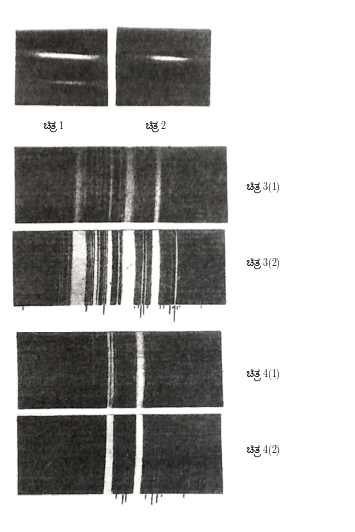
\includegraphics[scale=0.64]{"images/12.png"}
\caption{ಚದರುವಿಕೆಯ ದ್ರುವೀಕರಣ ಚಿತ್ರ \textbf{\general{\enginline{1}}}: ಸಂಸ್ಕರಣಗೊಳ್ಳದ ಚಿತ್ರ, ಚಿತ್ರ \textbf{\general{\enginline{2}}}: ಸಂಸ್ಕರಣಗೊಂಡ ಚಿತ್ರ, ಚಿತ್ರ \textbf{\general{\enginline{3(1)}}}: ಆಪಾತರೋಹಿತ ಚಿತ್ರ \textbf{\general{\enginline{3(2)}}}: ಚದರಿದ ರೋಹಿತ, ಚಿತ್ರ \textbf{\general{\enginline{4(1)}}}: ಆಪಾತರೋಹಿತ ಚಿತ್ರ \textbf{\general{\enginline{4(2)}}}: ಚದರಿದ ರೋಹಿತ. ರಾಮನ್ ರೋಹಿತದ \enginline{(Raman spectrum)} ರೇಖಾತ್ಮಕ ಗುಣವನ್ನು ಪ್ರದರ್ಶಿಸುವ ಮೊಟ್ಟಮೊದಲ ಚಿತ್ರ.}\label{chap5-fig07}
\end{figure}

ಅತಿ ಹೆಚ್ಚಿನ ಸಂಖ್ಯೆಯ ದ್ರವಗಳ ರೋಹಿತಗಳನ್ನೂ ಅಥವಾ ಈಗಾಗಲೇ ಪಡೆದ ಕ್ಯಾಮೆರಾ ಚಿತ್ರಗಳ ವಿಶ್ಲೇಷಣೆಯನ್ನೂ ಮಾಡಲು ಸಮಯವಿಲ್ಲದಾಗಿದೆ. ಆದರೂ ಬಹು ಸಂಖ್ಯೆಯ ದ್ರವಗಳ ರೋಹಿತವನ್ನು ವೀಕ್ಷಣೆ ಮಾಡಿದ್ದೇವೆ. ವಿವಿಧ ದ್ರವಗಳಲ್ಲಿ ಪಡೆದ ರೋಹಿತಗಳಲ್ಲಿ ಆಶ್ಚರ್ಯ ಹುಟ್ಟಿಸುವ ಹೋಲಿಕೆಗಳಿವೆ. \enginline{4358 A.U.} ತರಂಗಾಂತರದ ಕಿರಣವನ್ನು ಬಳಸಿದಾಗ ಚದರಿದ ಬೆಳಕಿನ ರೋಹಿತದಲ್ಲಿ ಸುಮಾರು \enginline{5000 A.U.} ತರಂಗಾಂತರದ ಕಿರಣವಾಗಿ ಮಾರ್ಪಾಡು ಗೊಂಡಿತು. ಇದು ಪೆಂಟೇನ್, ಹೆಕ್ಸೇನ್ ಮತ್ತು ಆಕ್ಟೇನ್‌ಗಳಲ್ಲಿ ಸಮಾನ ಅಂಶವಾಗಿತ್ತು. ಆದರೆ ಬೆನ್‍ಜೀನ್ ಅಥವಾ ನೀರನ್ನು ಬಳಸಿ ಪಡೆದ ರೋಹಿತದಲ್ಲಿ ಇವಕ್ಕಿಂತಲೂ ಬೇರೆಯಾಗಿತ್ತು. ಕ್ಪೀನೈನ್ ಸಲ್ಫೇಟ್ ದ್ರಾವಣವನ್ನು ಬಳಸಿ, ಪಾದರಸದ ಆರ್ಕ್ ಬೆಳಕಿನ \enginline{4047 A.U.} ಗೆರೆಯನ್ನು ಆಪಾತಗೊಳಿಸಿದಾಗ, ಅನೇಕ ದ್ರವಗಳಲ್ಲಿ ರೋಹಿತದ ನೀಲಿ ಭಾಗದಲ್ಲಿ ಎರಡನೇ ಗೆರೆ ಇರುವುದು ಕಂಡುಬಂದಿತು.

ಬೆನ್‍ಜೀನ್ ಮತ್ತು ಟಾಲೀನ್ ದ್ರವಗಳಲ್ಲಿ ಪಡೆದ ರೋಹಿತಗಳ ಚಿತ್ರಗಳಿಂದ ತಿಳಿದು ಬಂದ\-ದ್ದೆಂದರೆ, ಅವುಗಳಲ್ಲಿ ಕಾಣುವ ಅನೇಕ ಗೆರೆಗಳು ಜೋಡಿಗೆರೆಗಳಾಗಿರಬಹುದು.

ಬೆನ್‍ಜೀನ್ ಮತ್ತು ಟಾಲೀನ್ ಗಳಲ್ಲಿ ಪಡೆದ ರೋಹಿತಗಳ ಚಿತ್ರಗಳು ಒಂದಕ್ಕಿಂತಲೂ ಹೆಚ್ಚು ಮಾರ್ಪಾಡುಗೊಂಡ ಗೆರೆಗಳನ್ನು ತೋರಿಸುತ್ತವೆ. ಇವುಗಳಲ್ಲಿ ಕೆಲವು ಜೋಡಿಗೆರೆಗಳೂ ಇರಬಹುದು. ಅನೇಕ ದ್ರವಗಳ ರೋಹಿತಗಳಲ್ಲಿ, ಸ್ಪಷ್ಟಗೆರೆಗಳ ಜೊತೆಗೆ, ರೋಹಿತ ಪಟ್ಟಿಕೆಯೊಂದನ್ನೇ ತೋರಿಸು\-ವಂತಿದೆ. ಕಾರ್ಬನ್ ಡೈಸಲ್ಫೈಡ್ ವಿಚಿತ್ರವಾಗಿ ವರ್ತಿಸುತ್ತದೆ. ಇದರ ರೋಹಿತದಲ್ಲಿ ಅಸ್ಪಷ್ಟ ಪಟ್ಟಿಕೆಯಿದೆ.

ನಾವು ಇದುವರೆವಿಗೂ ಮಾಡಿದ ಪ್ರಯೋಗಗಳಲ್ಲಿ ಕಂಡ ಹೊಸ ಗೆರೆಗಳು ಧ್ರುವೀಕರಣಗೊಂಡಿವೆ. ಇದೂ ಅಲ್ಲದೆ ರೋಹಿತ ಪಟ್ಟಿಯೂ ಅಪೂರ್ಣವಾಗಿ ಧೃವೀಕರಣಗೊಂಡಿರುತ್ತದೆ.


\heading{ಹೊಸ ವಿಕಿರಣದ ಸ್ವರೂಪ}

ನಾನು ಹೇಳಿದ ಈ ಹೊಸ ಆವಿಷ್ಕಾರವು ಇನ್ನಷ್ಟು ಪ್ರಶ್ನೆಗಳಿಗೆ ಹಾದಿ ತೋರುತ್ತದೆ. ಮೊದಲ ಪ್ರಶ್ನೆಯೆಂದರೆ ನಾವು ಪಡೆದ ಮಾರ್ಪಾಡುಗೊಂಡ ವಿಕಿರಣವು ಉಂಟಾಗುವುದು ಹೇಗೆ? ದ್ರವದಲ್ಲಿನ ಅಣುಗಳಿಂದ ಚದರುವ ಬೆಳಕಿನ ಕಿರಣಗಳು ಹೊಸ ವಿಕಿರಣವಾಗುವುದು ಯಾವುದರಿಂದ? ಇವುಗಳಿಗೆ ತಾತ್ಕಾಲಿಕ ಉತ್ತರವಾಗಿ ಕ್ವಾಂಟಂ ಸಿದ್ಧಾಂತದ ಪರಿಭಾಷೆಯನ್ನು ನಾವು ಬಳಸಬೇಕು. ಆಪಾತ ಬೆಳಕಿನ ಕ್ವಾಂಟಂನ ಶಕ್ತಿಯನ್ನು ಅಣುವು ಆಂಶಿಕವಾಗಿ ಹೀರಿಕೊಂಡು ಉಳಿದದ್ದನ್ನು ಚದರಿಸುತ್ತದೆ. ಈ ಉತ್ತರವು ಅಸಂಬಂದ್ಧವೆನಿಸುವುದಿಲ್ಲ. ಏಕೆಂದರೆ ಕ್ರೇಮರ್\enginline{--} ಹೈಸನ್ ಬರ್ಗ್ ರವರ ಪ್ರಸರಣ (\enginline{dispersion}) ಸಿದ್ಧಾಂತವು ಈ ವಿದ್ಯಮಾನವನ್ನು ಈಗಾಗಲೇ ಸೂಚಿಸಿದೆ. ನಾವು ಈ ಸೂಚನೆಯನ್ನು ಆಧರಿಸಿ ಹೀಗೆ ಹೇಳಬಹುದು. ಆಪಾತ ಬೆಳಕಿನ ಕ್ವಾಂಟಂ ಮತ್ತು ಚದರಿದ ಬೆಳಕಿನ ಕ್ವಾಂಟಗಳ ನಡುವಿನ ವ್ಯತ್ಯಾಸವು, ಅಣುವು ಹೀರಿಕೊಂಡ ಕ್ವಾಂಟಂ ಶಕ್ತಿಯಿರಬಹುದು. ರೋಹಿತದಲ್ಲಿನ ಹೊಸ ಗೆರೆಗಳ ಆವೃತ್ತಿಯ ನಿಖರ ಅಳತೆಗಳು, ಅಣು ರೋಹಿತದ ಆವಕೆಂಪು ಭಾಗದಲ್ಲಿನ ಸಂಶೋಧನೆಗಳಿಗೆ ಹಾದಿ ತೆರೆಯುತ್ತದೆ.

ಆಪಾತ ವಿಕಿರಣದ ಕ್ವಾಂಟಂನ ಅಂಶವನ್ನು ಅಣುವು ಹೀರಿಕೊಂಡು ಉಳಿದದ್ದನ್ನು ಚದರಿಸುವುದು ಎಂದಾದರೆ, ಅದೇ ಅಣುವು ತನ್ನದೇ ವಿಶಿಷ್ಟ ಗುಣಹೊಂದಿದ ತರಂಗಾ ಆವೃತ್ತಿಯನ್ನು ಆಪಾತ ಕ್ವಾಂಟಂನ್ನು ಚದರಿಸುವಾಗ ದಾಟಿಸಲೂ ಬಹುದು. ಹೀಗಾದಲ್ಲಿ ನಾವು ರೋಹಿತದಲ್ಲಿನ ಗೆರೆಯು ಅಧಿಕ ತರಂಗಾ ಆವೃತ್ತಿಯ ಭಾಗದಲ್ಲಿರುತ್ತದೆ. ಈ ಬಗೆಯ ಗೆರೆಯನ್ನು ಚಿತ್ರ \enginline{3(2)} ರ ಎಡ ಭಾಗದಲ್ಲಿ ಕಾಣಬಹುದು. ಈ ಬಗೆಯ ವಿದ್ಯಮಾನವು ಇನ್ನಷ್ಟು ಪ್ರಯೋಗಗಳಿಂದ ಸಾಬೀತಾಗಬೇಕಾಗಿದೆ. ಇದುವರೆಗಿನ ಪ್ರಯೋಗಗಳಲ್ಲಿ ಬೆಳಕಿನ ಆವೃತ್ತಿಯು ಜಾಸ್ತಿಯಾಗು\-ವುದಕ್ಕಿಂತಲೂ ಕಡಿಮೆಯಾಗುವುದೇ ಕಂಡುಬಂದಿದೆ.

ಕೆಲವು ಪ್ರಯೋಗಗಳಲ್ಲಿ ಕಾಣಿಸಿದ ಅಭಿನ್ನ ರೋಹಿತ ಪಟ್ಟಿಕೆಯ ಬಗ್ಗೆ ಈಗ ಏನನ್ನೂ ಹೇಳಲಾಗುವು\-ದಿಲ್ಲ. ಇದು ಅಣುವಿನ ಮಾರ್ಪಾಡಿನಿಂದ ಉಂಟಾದದ್ದೇ ಅಥವಾ ಸ್ಥಿತಿಸ್ಥಾಪಕತೆ ಕಾಯ್ದುಕೊಳ್ಳಲಾಗದ ಎರಡನೆಯ ಬಗೆಯ ಅಣು ಘಟ್ಟನೆಗಳಿಂದಾದುದೇ ತಿಳಿದಿಲ್ಲ. ಹೀಗಾದಲ್ಲಿ ಆಪಾತ ಕ್ವಾಂಟಂನ ಆಂಶಿಕ ಶಕ್ತಿಯನ್ನು ಹೀರಿಕೊಂಡು ಅಣುಗಳ ಚಲನ ಶಕ್ತಿಯ ಮೇಲೆ ಪ್ರಭಾವ ಬೀರುವುದೇ ಎಂಬುದು ಪ್ರಶ್ನೆಯಾಗುತ್ತದೆ. ಇನ್ನಷ್ಟು ಪ್ರಯೋಗಗಳಿಂದ ಮಾಹಿತಿ ಸಂಗ್ರಹಗೊಂಡಾಗ ಈ ನಿಟ್ಟಿನಲ್ಲಿ ಸ್ಪಷ್ಟತೆ ಮೂಡುತ್ತದೆ. ಅಲ್ಲದೆ ಸಾಮಾನ್ಯ ಪ್ರತಿದೀಪ್ತಿಯಲ್ಲಿ ದ್ರಾವಕದ ಪಾತ್ರವೇನು ಎಂಬುದರ ಬಗ್ಗೆಯೂ ತಿಳಿಯುತ್ತದೆ.


\heading{ಉಷ್ಣಗತಿ ಶಾಸ್ತ್ರದೊಂದಿಗೆ ಸಂಬಂಧ}

ಪೀಠಕೆಯಲ್ಲಿ ಹೇಳಿದಂತೆ ಬೆಳಕಿನ ಸಾಮಾನ್ಯ ಚದರುವಿಕೆಯನ್ನು ಅಣುಗಳಿಂದ ಉಂಟಾದ ಪರಿಣಾಮವೆಂದು ಹೇಳಬಹುದು. ಹಾಗೆಯೇ ಇಡೀ ಮಾಧ್ಯಮದ ಉಷ್ಣಗತಿ ಏರಿಳಿತಗಳಿಂದ ಉಂಟಾದದ್ದೆಂದೂ ಅರ್ಥೈಸಬಹುದು. ಇಲ್ಲಿ ಏಳುವ ಪ್ರಶ್ನೆಯೆಂದರೆ, ನಾವು ಕಂಡ ದ್ವಿತೀಯಕ ವಿಕಿರಣವು ಅಣುಗಳಿಂದ ಮಾತ್ರ ಆದ ಪರಿಣಾಮವೇ ಅಥವಾ ಅಲ್ಲವೇ? ಮತ್ತು ಉಷ್ಣಗತಿ ಶಾಸ್ತ್ರಕ್ಕೆ ಈ ವಿದ್ಯಮಾನವು ಹೇಗೆ ಸಂಬಂಧಿಸಿದೆ? ಈ ಪ್ರಶ್ನೆಗಳನ್ನು ಸಿದ್ಧಾಂತ ಮತ್ತು ಪ್ರಯೋಗಗಳ ಮೂಲಕ ಶೋಧಿಸಬೇಕಾಗಿದೆ. ವಿವಿಧ ಉಷ್ಣತೆಗಳಲ್ಲಿ ಮತ್ತು ವಸ್ತುಗಳ ವಿವಿಧ ಭೌತಿಕ ಸ್ಥಿತಿಗಳಲ್ಲಿ ಪ್ರಯೋಗಗಳನ್ನು ಮಾಡಿ ಹೋಲಿಸುವುದು ಮುಖ್ಯವಾಗುತ್ತದೆ. ಅನಿಲಗಳಲ್ಲೂ ಮತ್ತು ಆವಿಗಳ\-ಲ್ಲಿಯೂ ಈ ಪರಿಣಾಮವನ್ನು ಗಮನಿಸಲಾಗಿದೆ ಎಂದು ಈ ಮೊದಲೇ ಹೇಳಿದ್ದೇನೆ. ಬೆಳಕಿನ ಧೃವೀಕರಣವನ್ನೂ ಮತ್ತು ತೀವ್ರತೆಯನ್ನೂ ಈ ಮಾಧ್ಯಮದಲ್ಲಿ ಅಳೆಯಲು ಸಾಧ್ಯವಾಗಿದೆ.\break ಘನಸ್ಥಿತಿಯ ನೀರಿನ ಸ್ಫಟಿಕವಾದ ಮಂಜುಗಡ್ಡೆಯೂ ಸಹ ಈ ಪರಿಣಾಮವನ್ನು ತೋರಿಸುತ್ತದೆ. ನೀರಿನಲ್ಲಿ ಪಡೆದ ರೋಹಿತದ ಗೆರೆಗಳಂತೆಯೇ ಮಂಜುಗಡ್ಡೆಯ ಚದರಿದ ಬೆಳಕಿನ ರೋಹಿತವಿರುವುದು ಆಶ್ವರ್ಯ ತರಿಸುತ್ತದೆ. ಸ್ಫಟಿಕವಲ್ಲದ ವಸ್ತುವನ್ನು ಪ್ರಯೋಗಕ್ಕೆ ಒಳಪಡಿಸಿರುವುದು ದ್ಯುತಿ ಗಾಜಿನಲ್ಲಿ ಮಾತ್ರ. ಇದರ ರೋಹಿತದಲ್ಲಿ ಗೆರೆಗಳಿಲ್ಲ. ಬದಲಿಗೆ ವಿಸರಿತ (\enginline{Diffuse}) ಪಟ್ಟಿಕೆಯಿರುತ್ತದೆ. ಇದು ಎಲ್ಲಾ ಅಸ್ಪಟಿಕ ವಸ್ತುಗಳಿಗೆ ಅನ್ವಯವಾಗುತ್ತದೆಯೇ ಅಥವಾ ಉಷ್ಣತೆಯ ಹೆಚ್ಚು ಕಡಿಮೆಗಳಿಗೆ ವ್ಯತ್ಯಯಗಳುಂಟಾಗುತ್ತವೆಯೇ? ಪ್ರಯೋಗಗಳೇ ನಿರ್ಣಯಿಸಬೇಕಿದೆ.


\heading{ಸಂಸಕ್ತ ಅಥವಾ ಅಸಂಸಕ್ತ ವಿಕಿರಣಗಳೇ?}

ಪ್ರಯೋಗಗಳಲ್ಲಿ ನಿರ್ಣಯಿಸಬೇಕಾದ ಬಹುಮುಖ್ಯ ಪ್ರಶ್ನೆಯೆಂದರೆ, ವಿವಿಧ ಬಗೆಯ\break ಅಣುಗಳಿಂದ, ಚದರುವಿಕೆಯಲ್ಲಿ ಮಾರ್ಪಾಡುಗೊಂಡ ವಿಕಿರಣಗಳು ಪರಸ್ಪರ ಅಸಂಸಕ್ತ\break (\enginline{Incoherant}) ವಾಗಿರುತ್ತವೆಯೇ. ಬಹುಷಃ ಹೀಗೆಯೇ ಇದ್ದಿರಬೇಕು. ಆದರೆ ಇಂಗಾಲದ ಡೈ ಆಕ್ಸೈಡ್ ಅನ್ನು ಉಕ್ಕಿನ ಪಾತ್ರೆಗಳಲ್ಲಿರಿಸಿ ಮಾಡಿದ ಪ್ರಯೋಗಗಳು ಈ ಆಲೋಚನೆಗೆ ತಡೆಯೊಡ್ಡುತ್ತವೆ. $\general{{\rm CO}}_2$ ಅನಿಲವನ್ನು, ಉಕ್ಕಿನ ಪಾತ್ರೆಯ ಬಿರಡೆ ತೆಗೆದು ಹೊರದಬ್ಬಿದಾಗ, ಪಾತ್ರೆಯೊಳಗೆ ಮೋಡ\-ವೊಂದು ಉಂಟಾಗುತ್ತದೆ. ಈ ಮೋಡವು ಬೆಳಕನ್ನು ಚದರಿಸುತ್ತದೆ. ಇದು ಸಾಮಾನ್ಯ ಚದರುವಿಕೆಯೇ ಆಗಿರುತ್ತದೆ. ಪೂರಕ ಸೋಸುಕದ ಮೂಲಕ ಈ ಮೋಡವನ್ನು ವೀಕ್ಷಿಸಿದಾಗ ತರಂಗ ಆವೃತ್ತಿಯಲ್ಲಿ ಮಾರ್ಪಾಡುಗೊಂಡ ಚದರಿದ ವಿಕಿರಣವು ಅಧಿಕ ಪ್ರಕಾಶ ಹೊಮ್ಮಿಸುತ್ತದೆ. ಅಂದರೆ ನಾವು ಈ ಹಿಂದೆ ಭಾವಿಸಿದ ಅಸಂಸಕ್ತತೆ ಇಲ್ಲವೆಂದಾಗುತ್ತದೆ. ಇದೂ ಅಲ್ಲದೆ ಮಿಥೈಲ್ ಆಲ್ಕೋಹಾಲ್ ಮತ್ತು ಕಾರ್ಬನ್ ಡೈಸಲ್‍ಫೈಡ್ ನ ಮಿಶ್ರಣವೂ ಸಹ ಯಾವುದೋ ಒಂದು ನಿರ್ಧಿಷ್ಟ ಉಷ್ಣತೆಯಲ್ಲಿ ಪ್ರಕಾಶ ಹೊಮ್ಮಿಸುತ್ತದೆ. ಆದರೆ ಅದನ್ನು ನಿಖರ ಮಾಪನ ಮಾಡಿದಾಗ ಮಾತ್ರ ಇನ್ನಷ್ಟು ಸತ್ಯ ತಿಳಿಯುತ್ತದೆ.


\heading{ಎಕ್ಸ್\general{\enginline{-}}ರೇ ಸಾದೃಶ ಸಾಧ್ಯತೆ}

ದೃಶ್ಯ ಭಾಗದ ರೋಹಿತದಲ್ಲಿನ ಕ್ವಾಂಟಂ ಅನ್ನು ಆಂಶಿಕವಾಗಿ ಹೀರಿಕೊಂಡು, ಮಿಕ್ಕಿದ್ದನ್ನು ಚದರಿಸುವ ಹಾಗಿದ್ದರೆ, ಎಕ್ಸ್\enginline{-}ರೇಗಳಲ್ಲೂ ಇದೇ ವಿದ್ಯಮಾನ ಉಂಟಾಗ ಬಾರದೇಕೆ? ಪ್ರೊಫೆಸರ್ ಕಾಂಪ್ಟನ್ ರವರು ಆವಿಷ್ಕರಿಸಿದ ಎಕ್ಸ್\enginline{-}ರೇ ಚದರುವಿಕೆಯು ತರಂಗ ಆವೃತ್ತಿಯನ್ನು ರೂಪಾಂತರ\-ಗೊಳಿಸುವ ಅನೇಕ ಬಗೆಯ ಚದರುವಿಕೆಗಳಲ್ಲೊಂದಾಗಿರಬಹುದು. ಇಂತಹವು ರೋಹಿತದಲ್ಲಿ ಗೆರೆ ಮೂಡಿಸುವಂತಿರಬಹುದು ಮಿಕ್ಕವು ನಿರಂತರ ತರಂಗಾಂತರದ ವಿಕಿರಣಗಳಾಗಿರಬಹುದು ರೋಹಿತದ ಅತಿ ನೀಲಭಾಗವು, ಪ್ರತಿದೀಪ್ತಿಯ ಬೆಳಕಿಗೆ ಹತ್ತಿರವಾದದ್ದು ಇದು ಹೊಸ ವಿಕಿರಣಗಳ ಬಗ್ಗೆ ಹೊಸ ಮಾಹಿತಿ ಹೊರಹಾಕಲು ಸಾಧ್ಯವಿದೆ.


\heading{ಕೊನೆಯದಾಗಿ}

ತರಂಗ ಸಿದ್ಧಾಂತ ಮತ್ತು ವಿಕಿರಣ ಸಿದ್ಧಾಂತ ಶಿಸ್ತುಗಳಲ್ಲಿನ ಅನೇಕ ಸಮಸ್ಯೆಗಳ ಬಗ್ಗೆ ಬೆಳಕು ಚೆಲ್ಲಬಹುದಾದ ಪ್ರಯೋಗ ಸಾಧ್ಯತೆಗಳ ಹೊಸ್ತಿಲಲ್ಲಿದ್ದೇವೆ. ಎಕ್ಸ್\enginline{-}ರೇ ದ್ಯುತಿ ಶಾಸ್ತ್ರ, ಅಣು ಮತ್ತು ಪರಮಾಣು ರೋಹಿತಗಳು, ಪ್ರತಿದೀಪ್ತಿ, ಚದರುವಿಕೆ, ರಸಾಯನಶಾಸ್ತ್ರ ಮತ್ತು ಉಷ್ಣಗತಿಶಾಸ್ತ್ರಗಳೂ ಈ ಪ್ರಯೋಗಗಳ ವ್ಯಾಪ್ತಿಯಲ್ಲಿ ಬರುತ್ತವೆ. ಇವುಗಳ ಬಗೆಗಿನ ಪ್ರಯೋಗಗಳನ್ನು ಕೈಗೆತ್ತಿಕೊಳ್ಳಬೇಕಾಗಿದೆ.

ನನ್ನ ಪ್ರಯೋಗಶಾಲೆಯ ಸಹಾಯ ಸಿಬ್ಬಂದಿ, ಕೆ.ಎಸ್.ಕ್ರಿಷ್ಣನ್ ಮತ್ತು ಎಸ್. ವೆಂಕಟೇಶ್ವರನ್ ರವರ ನೆರವನ್ನು ಈ ಸಂಶೋಧನೆಯ ಕಾರ್ಯಕ್ಕಾಗಿ ನೆನೆಯುತ್ತೇನೆ. ಇವರಿಗೆ ಆಭಾರಿಯಾಗಿದ್ದೇನೆ.

\enginline{28} ಫೆಬ್ರವರಿ, \enginline{1928} ರ ದಿನದಂದು ಹೊಸವಿಕಿರಣದ ಗೆರೆಗಳುಳ್ಳ ರೋಹಿತವನ್ನು ವೀಕ್ಷಿಸ\-ಲಾಯಿತು. ಮಾರನೆ ದಿನ ಈ ವಿಷಯವನ್ನು ಪ್ರಚಾರ ಪಡಿಸಲಾಯಿತು.


\heading{ಡೇವಿಸನ್‍ರವರು ರಾಮನ್‍ರವರ ಬಗ್ಗೆ}

ರಾಮನ್‍ರವರ ಆವಿಷ್ಕಾರದ ಬಗ್ಗೆ ಒಂದು ನೇರ ನುಡಿಯ ಪ್ರಬಂಧವನ್ನು ಸಿ.ಜಿ.ಡೇವಿಸನ್‌ರವರು \enginline{1931}ರಲ್ಲಿ ಬೆಲ್ ಲ್ಯಾಬೊರೇಟರೀಸ್ ರೆಕಾರ್ಡ್‌ನಲ್ಲಿ ಬರೆದರು. ಆಗ ರಾಮನ್‍ರವರಿಗೆ ನೊಬೆಲ್ ಬಹುಮಾನ ಬಂದಿತ್ತು. ಡೇವಿಸನ್ ಬೆಲ್ ಲ್ಯಾಬೊರೇಟರೀಸ್‌ನಲ್ಲಿಯೇ ಸಂಶೋಧಕರಾಗಿದ್ದರು. ಐದು ವರ್ಷಗಳ ಬಳಿಕ ಡೇವಿಸನ್, ಜಿ. ಪಿ. ಥಾಮ್ಸನ್ ರವರೊಡನೆ ಎಲೆಕ್ಟ್ರಾನ್ನ ತರಂಗ ಸ್ವರೂಪದ ಬಗ್ಗೆ ನೊಬೆಲ್ ಬಹುಮಾನ ಪಡೆದುಕೊಂಡರು. ಇವರ ಪ್ರಬಂಧದ ಸಂಕ್ಷೇಪ ರೂಪವನ್ನು ಈ ಪುಸ್ತಕದ ಮೊದಲ ಅಧ್ಯಾಯಗಳಲ್ಲಿ ನೀಡಿದೆ. ಇಲ್ಲಿ ಇದರ ಪೂರ್ಣಪಾಠವನ್ನು ನೀಡುತ್ತಿದ್ದೇನೆ.

\enginline{1930}ರಲ್ಲಿ  ಸರ್ ಸಿ.ವಿ. ರಾಮನ್‍ರವರಿಗೆ ನೊಬೆಲ್ ಬಹುಮಾನವನ್ನು ನೀಡಿ ಸ್ವೀಡಿಷ್ ಅಕಾಡೆಮಿ ಆಫ಼್ ಸೈನ್ಸಸ್ ಒಳ್ಳೆಯ ಕೆಲಸ ಮಾಡಿದೆ. ಜಗತ್ತಿನಾದ್ಯಂತ ವಿಜ್ಞಾನಿಗಳು ರಾಮನ್ ಪರಿಣಾಮವು ಇತ್ತೀಚಿನ ದಿನಗಳ ಸಂಶೋಧನೆಯಲ್ಲಿ ಹಿರಿಯ ಆವಿಷ್ಕಾರವೆಂಬ ಅಭಿಪ್ರಾಯಕ್ಕೆ ಮಾನ್ಯತೆ ನೀಡಿದೆ.

ಈ ನೊಬೆಲ್ ಬಹುಮಾನವು, ಹಿಂದಿನ ಪದ್ಧತಿಯಂತೆ, ಒಂದೇ ಒಂದು ಪ್ರಯೋಗದ ಫಲಿತಾಂಶಕ್ಕಾಗಿ ನೀಡಲಾಗಿದೆ. ಈ ಫಲಿತಾಂಶವು ಅಷ್ಟು ಘನವಾಗಿದೆಯೆಂಬುದೂ ವೇದ್ಯವಾಗುತ್ತದೆ. ಹಿಂದೆ ಬಹುಮಾನ ಗಳಿಸಿದ ಪ್ರಯೋಗಗಳಂತೆ, ಇದೂ ಸಹ ಬಹಳ ಸರಳ ಪ್ರಯೋಗವೇ ಆಗಿದೆ. ಈ ಪ್ರಯೋಗವನ್ನು ಯಾವ ಭೌತಶಾಸ್ತ್ರದ ಪ್ರಯೋಗಾಲಯಗಳಲ್ಲೂ, ಯಾವ ಸಮಯದಲ್ಲೂ ಕಳೆದ ನಲವತ್ತು, ಐವತ್ತು ವರ್ಷಗಳಲ್ಲಿ ಮಾಡಬಹುದಾಗಿತ್ತು. ರಾಮನ್‍ರವರು ತಮ್ಮ ಆವಿಷ್ಕಾರವನ್ನು ಘೋಷಿಸಿದ ವರ್ಷವೇ ಸುಮಾರು \enginline{40} ಜನ ಸಂಶೋಧಕರು ಇದೇ ಪ್ರಯೋಗ ಮಾಡಿ ಫಲಿತಾಂಶವನ್ನು ಸಾಬೀತು ಮಾಡಿದ್ದಾರೆ.

ಈ ಪ್ರಯೋಗದಲ್ಲಿ, ಒಂದು ಪಾರದರ್ಶಕ ವಸ್ತುವಿನ ಮೂಲಕ ಏಕತರಂಗ ಕಿರಣವನ್ನು ಹಾಯಿಸಲಾಗುತ್ತದೆ. ಈ ಬೆಳಕನ್ನು ವಸ್ತುವು ಚದರಿಸುತ್ತದೆ. ಚದರಿದ ಬೆಳಕಿನ ರೋಹಿತವನ್ನು ಪಡೆದಾಗ, ರಾಮನ್‍ರವರಿಗೆ ಆ ವಸ್ತುವಿನ ರೋಹಿತದಲ್ಲಿ ಇರಬೇಕಾದ ಗೆರೆಗಳಿಗಿಂತಲೂ ಹೆಚ್ಚಿನ ಗೆರೆಗಳು ಕಂಡವು. ಈ ಹೆಚ್ಚಿನ ಗೆರೆಗಳು ಮೂಲ ಗೆರೆಗಳಿಗೆ ಉಪಗ್ರಹಗಳೆಂಬಂತೆ ಇದ್ದವು. ಮುಖ್ಯ ಗೆರೆಗಳಿಗೆ ಕೊಂಚದೂರದಲ್ಲಿ ಇವುಗಳು ಕಂಡು ಬಂದವು. ಅಂದರೆ ಮುಖ್ಯ ಗೆರೆಗಳ ಸ್ಥಾನ ಬದಲಿಸಿದಾಗ, ಈ ಉಪಗ್ರಹದಂತಹ ಗೆರೆಗಳು ಅಷ್ಟೇ ದೂರದಲ್ಲಿ ಸ್ಥಾನ ಬದಲಿಸಿಕೊಂಡವು.

ಮರ್ಕ್ಯುರಿ ಆರ್ಕ್ ಕಿರಣಗಳನ್ನು ಬಳಸಿ, ರಾಮನ್‍ರವರು ಅನೇಕ ಸಾವಯವ ವಸ್ತುಗಳ ರೋಹಿತಗಳನ್ನು ಪಡೆದರು. ದೀರ್ಘಕಾಲದವರೆಗೆ ರೋಹಿತಪಟ್ಟಕವನ್ನು ಪಡೆದರು. ಇದರಲ್ಲಿ ಹೆಚ್ಚಿನ ಗೆರೆಗಳು ಅಥವಾ ಸೆಕೆಂಡರಿ ಗೆರೆಗಳು ಕಂಡು ಬಂದವು. ಹೆಚ್ಚಿನ ವಿಶ್ಲೇಷಣಕ್ಕೆ ಒಳಪಡಿಸಿದಾಗ ಈ ಸೆಕೆಂಡರಿ ಗೆರೆಗಳು ಯಾವ ಮುಖ್ಯ ಗೆರೆಗಳ ಸಂವಾದಿಯಾಗಿದೆ ಎಂಬುದು ತಿಳಿಯಿತು. ಅಲ್ಲದೆ ಈ ಸಂವಾದಿ ಗೆರೆಗಳು, ಮುಖ್ಯ ಗೆರೆಗಳಿಂದ ನಿರ್ದಿಷ್ಟ ಆವೃತ್ತಿಯಿಂದ ಬೇರೆಯಾಗಿರುವುದು ಕಂಡು ಬಂದಿತು. ಕೆಲವೊಮ್ಮೆ ರೋಹಿತ ಪಟ್ಟಿಯಲ್ಲಿ ಒಂದರ ಮೇಲೊಂದು ಗೆರೆಗಳಾದರೂ ಸಹ, ನಿರ್ದಿಷ್ಟ ಆವೃತ್ತಿಯ ಭಿನ್ನತೆಯನ್ನು ಪತ್ತೆಹಚ್ಚುವುದು ಕಷ್ಟವಾಗಲಾರದು. ಇನ್ನೊಂದು ಬಗೆಯಲ್ಲಿ ಮುಖ್ಯ ಗೆರೆಗಳ ಆಚೀಚೆಯೂ ಸೆಕೆಂಡರಿ ಗೆರೆಗಳು ಇರಬಹುದು. ಕಂಡು ಬಂದ ನಿಯಮದಂತೆ ಸೆಕೆಂಡರಿ ಗೆರೆಗಳ ದಟ್ಟಣೆ ಕಡಿಮೆ ಆವೃತ್ತಿಯ ಕಡೆಗೇ ಇರುತ್ತದೆ. ಹೆಚ್ಚಿನ ಆವೃತ್ತಿಯಿರುವ ಗೆರೆಗಳು ಮುಖ್ಯಗೆರೆಗಳ ಪಕ್ಕ ಕಂಡು ಬಂದರೂ ಸಹ ಅವುಗಳಿಗೂ ಮುಖ್ಯ ಗೆರೆಗಳ ಆವೃತ್ತಿಗೂ ಇರುವುದು ನಿರ್ದಿಷ್ಟ ವ್ಯತ್ಯಾಸವೇ. ಅಲ್ಲದೆ ಇದೇ ನಿರ್ದಿಷ್ಟ ವ್ಯತ್ಯಾಸವೇ ಕನಿಷ್ಟ ಆವೃತ್ತಿಯಿರುವ ಗೆರೆಗಳು ಮತ್ತು ಮುಖ್ಯ ಗೆರೆಗಳಿಗೂ ಕಂಡುಬರುತ್ತದೆ. ಆಪಾತ ಬೆಳಕಿನ ಕಿರಣಗಳ ಆವೃತ್ತಿಗೆ, ಒಂದು ನಿರ್ದಿಷ್ಟ ಮೊತ್ತವನ್ನು ಸೇರಿಸಿ ಚದರಿಸುವುದು ಅಥವಾ ಅದೇ ನಿರ್ದಿಷ್ಟ ಮೊತ್ತವನ್ನು ಕಳೆದು ಚದರಿಸುವುದು ವಸ್ತುವು ಮಾಡುತ್ತಿದೆ ಎಂದು ಸಾಬೀತಾಗುತ್ತದೆ.

ಈ ಸರಳ ಲೆಕ್ಕಾಚಾರಗಳು ರಾಮನ್ ಪರಿಣಾಮವನ್ನು ಮಿಕ್ಕ ಪ್ರತಿದೀಪ್ತಿ ಪರಿಣಾಮಗಳಿಗಿಂತಲೂ ಭಿನ್ನವಾಗಿರುವನ್ನು ಎತ್ತಿ ತೋರಿಸುತ್ತದೆ, ಅಲ್ಲದೆ ಪ್ರತಿದೀಪ್ತಿ ವಿದ್ಯಮಾನವು ಕೆಲವೇ ವಸ್ತುಗಳಲ್ಲೋ/ಖನಿಜಗಳಲ್ಲೋ ಕಂಡುಬರುತ್ತದೆ. ರಾಮನ್ ಪರಿಣಾಮವು ವಿಶ್ವಮಾನ್ಯ ಪರಿಣಾಮ. ಎಲ್ಲ ಪಾರದರ್ಶಕ ವಸ್ತುಗಳಲ್ಲೂ ಅವರು ಘನ, ದ್ರವ ಅಥವಾ ಅನಿಲಗಳಾಗಿದ್ದರೂ ಈ ಪರಿಣಾಮವು ಸಾಬೀತಾಗುತ್ತದೆ.

ರಾಮನ್ ಪರಿಣಾಮದ ಲೆಕ್ಕಾಚಾರಗಳು ಮತ್ತು ಮುಂದೆ ವಿವರಿಸಲಾಗುವ ಪರಿಣಾಮವೂ ಸಹ ಬೆಳಕಿನ ಕ್ವಾಂಟಾ ಮತ್ತು ಈಗಾಗಲೇ ತಿಳಿದಿರುವ ಅಣುಗಳ ಲಕ್ಷಣಗಳ ಮೂಲಕ ವಿವರಿಸಬಹುದಾಗಿದೆ. ಈ ಒಂದು ಕಾರಣಕ್ಕಾಗಿಯೇ ರಾಮನ್ ಪರಿಣಾಮದ ಆವಿಷ್ಕಾರವನ್ನು ಬಹುಮುಖ್ಯ ಸಂಶೋಧನೆ\-ಯೆಂದು ಪರಿಗಣಿಸಬೇಕಾಗುತ್ತದೆ. ಬೆಳಕಿನ ಕಿರಣವನ್ನು ತರಂಗಗಳಂತೆಯೂ, ಕಣಗಳಂತೆಯೂ ವಿವರಿಸುವ ಅನೇಕ ದ್ಯುತಿ ಪ್ರಯೋಗ ಮತ್ತು ಪರಿಣಾಮಗಳ ಪಟ್ಟಿಗೆ ರಾಮನ್ ಪರಿಣಾಮವನ್ನು ಸಹ ಸೇರಿಸಬೇಕಾಗುತ್ತದೆ.

ದ್ಯುತಿವಿದ್ಯುತ್ ಪರಿಣಾಮ ಕುರಿತ ಐನ್‍ಸ್ಟೈನ್ ಸಿದ್ಧಾಂತವು ಬೆಳಕಿನ ಕಣ ಸಿದ್ಧಾಂತಕ್ಕೆ ಮರುಜೀವ ನೀಡಿತು. \enginline{1924} ಕಾಂಪ್ಟನ್ ಪರಿಣಾಮವು ಕಣಸಿದ್ಧಾಂತ ಮತ್ತು ತರಂಗ ಸಿದ್ಧಾಂತಗಳ ನಡುವಿನ ವೈರುದ್ಧ್ಯಗಳಲ್ಲಿ ಓಲಾಡುವಂತಾಯಿತು. ಆಯಾ ಪರಿಣಾಮಗಳಿಗೆ ಹೊಂದುವ ಹಾಗೆ ಕಣ ಮತ್ತು ತರಂಗಗಳ ಪರಿಧಿಯಲ್ಲಿ ವಿದ್ಯಮಾನಗಳನ್ನು ವಿವರಿಸುವಂತಾಯಿತು. ಹೀಗಾದಾಗಲೂ ಕಣಗಳು ಮತ್ತು ತರಂಗಗಳ ನಡುವಿನ ಸಂಬಂಧಗಳನ್ನು ವಿವರಿಸಲು ಈಗಾಗಲೇ ಚಾಲ್ತಿಯಲ್ಲಿರುವ ಎರಡು ಭೌತಶಾಸ್ತ್ರಗಳ ನಿಯಮಗಳನ್ನು ಬಳಸುತ್ತೇವೆ. ಬೆಳಕಿನ ಕಣಗಳು ಅಂದರೆ ಫೋಟಾನುಗಳ ಶಕ್ತಿಯ ತರಂಗಗಳ ಆವೃತ್ತಿ (ಸೆಕೆಂಡಿಗೆ ಎಷ್ಟು ತರಂಗಗಳು), ಅನುಪಾತದಲ್ಲಿರುತ್ತದೆ. ಈ ಅನುಪಾತದ ನಿರ್ದಿಷ್ಟ ಸಂಖ್ಯೆ ಪ್ಲಾಂಕ್ ಕಾನ್ ಸ್ಟೆಂಟ್ \enginline{h} ಆಗಿರುತ್ತದೆ.

ಕಣ ಸಿದ್ಧಾಂತದ ಪ್ರಕಾರ ರಾಮನ್ ಪರಿಣಾಮವನ್ನು ಈ ಬಗೆಯಲ್ಲಿ ವಿವರಿಸಬಹುದು. ಆಪಾತ ಬೆಳಕಿನ ಕಿರಣಗಳ ಫೋಟಾನುಗಳು, ಅಣುಗಳ ಮೇಲೆ ಬಿದ್ದಾಗ ಅವು ಉಂಟು ಮಾಡುವ ಪರಿ\-ಣಾಮವು ರಾಮನ್ ಎಫೆಕ್ಟ್ ಆಗುತ್ತದೆ. ಅಣುಗಳ ಮೇಲೆ ಸಂಘಟಿಸಿದ ಫೋಟಾನುಗಳು, ಶಕ್ತಿಯನ್ನು ಕಳೆದುಕೊಂಡು ಹೊರಚಿಮ್ಮುತ್ತದೆ. ಇವೇ ಬೆಳಕಿನ ಚದುರಿಕೆಯ ವಿದ್ಯಮಾನವಾಗುತ್ತದೆ. ಇದನ್ನೇ ವ್ಯತ್ಯಯಗೊಂಡ ಆವೃತ್ತಿಯ ಬೆಳಕೆಂದು ರಾಮನ್ ಆವಿಷ್ಕರಿಸಿದ್ದು. ಪ್ರತಿಯೊಂದು ಅಣುವಿಗೂ ಈ ವಿಶೇಷ ಲಕ್ಷಣವಿರುತ್ತದೆ.

ಅಣುಗಳ ಆಂತರಿಕ ಶಕ್ತಿಯು ಕೆಲವು ನಿರ್ದಿಷ್ಟ ಮಟ್ಟಗಳಲ್ಲಿರಲು ಮಾತ್ರ ಸಾಧ್ಯ. ಅಣುಗಳ ಕೆಲವು ಶಕ್ತಿ ಮಟ್ಟಗಳಲ್ಲಿ ಮಾತ್ರ ತಮ್ಮ ಸ್ಥಿರತೆಯನ್ನು ಹೊಂದಿರುತ್ತವೆ. ಹೊರಗಿನಿಂದ ಬಂದ ಶಕ್ತಿಯನ್ನು ಇವು ಒಳಕ್ಕೆ ಸೆಳೆದು ಕೊಳ್ಳಬಹುದು ಅಥವಾ ಹೊರಗೆ ಹಾಕಬಹುದು. ಆಗ ಅಣುವಿನ “ಶಕ್ತಿಯ ಮಟ್ಟಗಳಲ್ಲಿ ವ್ಯತ್ಯಯವುಂಟಾಗುತ್ತದೆ. ಹೀಗೆ ಸಂಘಟ್ಟಿಸಿದ ಫೋಟಾನ್‍ಗಳು, ಅಣುಗಳಿಗೆ ಅವುಗಳ ಶಕ್ತಿ ಮಟ್ಟವನ್ನೂ ಏರಿಕೆ ಅಥವಾ ಇಳಿಕೆ ಮಾಡಬಲ್ಲವು. ಫೋಟಾನು ಶಕ್ತಿ ಹೀರಿದ ಅಣುವು ಮೇಲ್ಮಟ್ಟದ ಶಕ್ತಿಯಿಂದ ಕೆಳಮಟ್ಟಕ್ಕೆ ಇಳಿಯುವಾಗ ಹೊರಹಾಕುವ ಶಕ್ತಿಯು ಫೋಟಾನ್ ರೂಪದಲ್ಲಿಯೇ ಇರುತ್ತದೆ. ಹಾಗಾಗಿ ಹೊರಬಿದ್ದ ಫೋಟಾನ್‍ಗಳು, ಆಪಾತ ಫೋಟಾನ್‌ಗಳೊಂದಿಗೆ ಹೋಲಿಸಿದಾಗ ತೋರಿಸುವ ಶಕ್ತಿ ವ್ಯತ್ಯಯವು, ಅಣುಗಳ ಶಕ್ತಿ ಮಟ್ಟಗಳನ್ನು ನಿಖರವಾಗಿ ಗುರುತಿಸಬಲ್ಲುದು. ರಾಮನ್ ರೋಹಿತದಲ್ಲಿ\break \enginline{(Raman spectrum)} ಕಾಣುವ ಸ್ಪಷ್ಟ ಗೆರೆಗಳಿಗೆ ಇದುವೇ ಕಾರಣ. ಹೀಗೆ ಅಣುಗಳ ಶಕ್ತಿ ಮಟ್ಟ ತಿಳಿದಿದ್ದರೆ ರಾಮನ್ ರೋಹಿತದ ಫೋಟಾನ್‍ಗಳು ಹೊಂದಿದ ವ್ಯತ್ಯಯಗಳನ್ನು ಗುರುತಿಸಲು ಸಾಧ್ಯವಾಗುತ್ತದೆ.

ಅಧಿಕ ಆವೃತ್ತಿಯ ರಾಮನ್ ರೋಹಿತದಲ್ಲಿನ \enginline{(Raman spectrum)} ಗೆರೆಗಳನ್ನು ಹೀಗೆಯೇ ವಿವರಿಸಲು ಸಾಧ್ಯವಾಗುತ್ತದೆ. ಒಂದು ಫೋಟಾನ್‍ಗೆ ಅಣುವನ್ನು ಸಂಘಟ್ಟಿಸಿದಾಗ, ಅಣುವಿನ ಶಕ್ತಿ ಮಟ್ಟವನ್ನು ಹೆಚ್ಚಿಸಲು ಸಾಧ್ಯವಾಗುವುದಾದರೆ, ಅದೇ ಅಣುವಿಗೆ ಇನ್ನೊಂದು ಫೋಟಾನ್‍ಗೆ ಹೆಚ್ಚಿನ ಶಕ್ತಿಯನ್ನು ಒದಗಿಸಲೂ ಸಾಧ್ಯವಾಗಬೇಕು. ಈ ವಿದ್ಯಮಾನವನ್ನು ಎಲೆಕ್ಟ್ರಾನ್ ಮತ್ತು ಅಣುಗಳ ನಡುವಿನ ಎರಡನೆಯ ಬಗೆಯ ಸಂಘಟ್ಟನ ವಿನಿಮಯ ಎನ್ನುತ್ತೇವೆ. ರಾಮನ್ ರೋಹಿತ \enginline{(Raman spectrum)} ಗೆರೆಗಳಲ್ಲಿ ಅತಿಹೆಚ್ಚು ಆವೃತ್ತಿಯ ಗೆರೆಗಳಿಗೆ ಸಂವಾದಿಯಾಗಿ, ಕನಿಷ್ಠ ಆವೃತ್ತಿಯ ಗೆರೆಗಳಿರುವುದು ಈ ಬಗೆಯ ವಿದ್ಯಮಾನದಿಂದಾಗಿ. ಇವು ಕ್ಷೀಣ ರೋಹಿತವಾಗಿ ತೋರುವುದೇಕೆಂದರೆ ಸಾಮಾನ್ಯ ಸ್ಥಿತಿಯಲ್ಲಿ ವಸ್ತುವಿನ ಅಣುಗಳು ಕನಿಷ್ಠ ಮಟ್ಟದ ಶಕ್ತಿಯಲ್ಲಿಯೇ ಇರುತ್ತವಾದ್ದರಿಂದ ತಮ್ಮ ಶಕ್ತಿಯನ್ನು ವಿನಿಮಯ ಮಾಡಿಕೊಳ್ಳಲಾರದ ಸ್ಥಿತಿಯಲ್ಲಿರುತ್ತವೆ.

ಹೀಗೆ ರಾಮನ್ ಪರಿಣಾಮದ ಪ್ರಾಮುಖ್ಯ ಇರುವುದು ಇಲ್ಲಿ. ನಮ್ಮ ಅರಿವಿಗೆ ಬಾರದ ಪ್ರಕೃತಿಯ ಈ ವಿದ್ಯಮಾನವನ್ನು ನಮಗೆ ತಿಳಿಯ ಪಡಿಸಿರುವುದು. ಫೋಟಾನ್‍ನ ಇರುವಿಕೆಯನ್ನು ಸಾಬೀತು ಪಡಿಸಿರುವುದು ಒಂದು ಭಾಗವಾದರೆ, ಅಣುಗಳ ಶಕ್ತಿ ಮಟ್ಟವನ್ನು ತಿಳಿದುಕೊಳ್ಳುವುದು ಇನ್ನೊಂದು ಭಾಗ.

ಈ ಹಿಂದೆ ಹೇಳಿದಂತೆ, ರಾಮನ್ ಪರಿಣಾಮವನ್ನು ತಿಳಿಯಪಡಿಸುವ ಪ್ರಯೋಗವನ್ನು\break ಯಾವುದೇ ಭೌತ ವಿಜ್ಞಾನದ ಪ್ರಯೋಗಾಲಯಗಳಲ್ಲಿ ಹಲವು ದಶಕಗಳ ಮೊದಲೇ ಮಾಡಬಹು\-ದಾಗಿತ್ತು. ಇದು ಅಂತಹ ಸರಳ ಪ್ರಯೋಗ. ರಾಮನ್‍ರವರೇ ಈ ಪ್ರಯೋಗ ಮಾಡಿದ್ದು ಆಕಸ್ಮಿಕವೇನಲ್ಲ. ಭೌತಶಾಸ್ತ್ರದಲ್ಲಿನ ಅತಿ ಪ್ರಮುಖ ಸಂಶೋಧನೆಗಳು, ಅದರಲ್ಲಿಯೂ ಅತಿ ಸರಳವೆನ್ನಿಸುವ ಪ್ರಯೋಗಗಳು ವೈಜ್ಞಾನಿಕ ಕಾರ್ಯದಲ್ಲಿ ನಿರಂತರವಾಗಿ ತೊಡಗಿರುವವರಿಗೆ ಮಾತ್ರ ದಕ್ಕಬಲ್ಲದು. ಇತರರಿಗಲ್ಲ. ಈ ಪರಿಣಾಮವು ಇದಕ್ಕೆ ಅಪವಾದವಲ್ಲ. ಬೆಳಕಿನ ಚದರುವಿಕೆಯ ಬಗ್ಗೆ ನಿರಂತರವಾಗಿ ಪ್ರಯೋಗ ನಿರತರಾಗಿರುವವರು ರಾಮನ್‍ರವರೊಬ್ಬರೇ. \enginline{1907}ರಲ್ಲಿ ಮದರಾಸಿನ ಪ್ರೆಸಿಡೆನ್ಸಿ ಕಾಲೇಜಿನಿಂದ ಪದವೀಧರರಾದ ಮೇಲೆ ಅವರೇ ಪ್ರಕಟಿಸಿರುವ ಹೊತ್ತಿಗೆಗಳಿಂದ\enginline{--} ಕಂಡು\-ಬರುವ ಅಂಶವೆಂದರೆ\enginline{--}ಯಾಂತ್ರಿಕ ಕಂಪನಗಳು. ಸಂಗೀತ ವಾದ್ಯಗಳು ಮತ್ತು ಶಬ್ದ ಸಂಬಂಧಿತ ಸಮಸ್ಯೆಗಳ ಬಗ್ಗೆ ಅವರು ಆಸಕ್ತರಾದರು. ಈ ಅವಧಿಯಲ್ಲೂ ಸಹ ಬೆಳಕಿನ ಬಗೆಗಿನ ಸಮಸ್ಯೆಗಳ ಬಗ್ಗೆಯೂ ಅವರ ಒಲವಿತ್ತು. \enginline{1920}ರ ಸುಮಾರಿನಲ್ಲಿ ಅಂದರೆ, ಅವರು ಪಾಲಿತ್ ಪ್ರಾಧ್ಯಾಪಕರೆಂದು ಕಲ್ಕತ್ತ ಯೂನಿವರ್ಸಿಟಿಯಲ್ಲಿ ನೇಮಕಗೊಂಡ ಮೂರು ವರ್ಷಗಳ ತರುವಾಯ ಅವರು ಶಬ್ದ ಸಂಬಂಧಿತ ಅಧ್ಯಯನದಿಂದ ದ್ಯುತಿ ವಿಶ್ಲೇಷಣೆಗೆ ಆಸಕ್ತಿ ಬದಲಿಸಿಕೊಂಡರು. ಅದರಲ್ಲೂ ಬೆಳಕಿನ ಚದರುವಿಕೆಯ ಬಗ್ಗೆ ತೀವ್ರ ನಿಷ್ಠೆ ತೋರಿದರು. ಅವರು ಪ್ರಯೋಗಶೀಲರಾದದ್ದೇ ಅಲ್ಲದೆ ಸೈದ್ಧಾಂತಿಕವಾಗಿಯೂ ಕಾರ್ಯ ಪ್ರವೃತ್ತರಾದರು. ಒಂದು ನೂರಕ್ಕೂ ಹೆಚ್ಚಿನ ಪ್ರಬಂಧಗಳನ್ನು ರಾಮನ್ ಮತ್ತು ಅವರ ಸಹೋದ್ಯೋಗಿಗಳು ಪ್ರಕಟಿಸಿದ್ದಾರೆ. ಇವುಗಳಲ್ಲಿ \enginline{83} ಬೆಳಕಿನ ಬಗ್ಗೆಯೂ, \enginline{49} ಬೆಳಕಿನ ಚದರುವಿಕೆಯ ಬಗ್ಗೆಯೂ ಇವೆ.

ಇದು ಭಾರತದಲ್ಲಿ ವಿಜ್ಞಾನದ ಮುನ್ನಡೆಯನ್ನು ತೋರಿಸುತ್ತದೆ. ಅಲ್ಲದೆ ರಾಮನ್‍ರವರು ತಮ್ಮ ವಿದ್ವತ್ತಿಗೆ ಹೊರದೇಶಗಳ ಯಾವ ಭೌತಶಾಸ್ತ್ರಜ್ಞರಿಂದಲೂ ಸಹಾಯ ಪಡೆದಿಲ್ಲ. ರಾಮನ್‍ರವರ ವಿಜ್ಞಾನ ಶಿಕ್ಷಣವು ಭಾರತದಲ್ಲೇ ಆಗಿದೆ, ಒಂದು ವರ್ಷ ಹೊರತುಪಡಿಸಿದರೆ ಮಿಕ್ಕೆಲ್ಲ ಜೀವನವನ್ನು ತಮ್ಮ ದೇಶದಲ್ಲೇ ಸವೆಸಿದ್ದಾರೆ. \enginline{1924}ರಲ್ಲಿ ಟೊರೆಂಟೋದಲ್ಲಿ ನಡೆದ ಬ್ರಿಟಿಷ್ ಅಸೋಸಿಯೇಷನ್‍ನ\break ಮೀಟಿಂಗ್‍ಗೆ ಬಂದಿದ್ದರು. ಹಾಗೆಯೇ ಕ್ಯಾಲಿಫೋರ್ನಿಯಾ ಇನ್ಸ್‌ಟಿಟ್ಯೂಟ್ ಆಫ಼್ ಟೆಕ್ನಾಲಜಿಯಲ್ಲಿ ಕೆಲವು ತಿಂಗಳ ಕಾಲ ಸಂಶೋಧನೆಯಲ್ಲಿ ತೊಡಗಿದ್ದರು.

ರಾಮನ್‍ರವರಿಗೆ ಅನೇಕ ಪ್ರಶಸ್ತಿಗಳು ಬಂದಿವೆ. ಅವರು ಇಂಡಿಯನ್ ಸಯನ್ಸ್ ಕಾಂಗ್ರೆಸ್‍ಗೆ ಸಾಮಾನ್ಯ ಅಧ್ಯಕ್ಷರಾಗಿದ್ದಾರೆ. ರಾಯಲ್ ಸೊಸೈಟಿಯಲ್ಲಿ ಫೆಲೋ ಆಗಿದ್ದಾರೆ. ಕಿಂಗ್ ಜಾರ್ಜ್ ರವರಿಂದ ನೈಟ್ ಹುಡ್ \enginline{1929}ರಲ್ಲಿ ಸಿಕ್ಕಿದೆ. ಚಂದ್ರಶೇಖರ ವೆಂಕಟ ರಾಮನ್‍ರವರಿಗೆ ನೊಬೆಲ್ ಪ್ರಶಸ್ತಿ ಬಂದಿರುವುದು ಭಾರತಕ್ಕೆ ಬಂದ ಮೊದಲ ನೊಬೆಲ್ ಕೀರ್ತಿಯಾಗಿದೆ”.

